% % Preamble BEGINN %%%%%%%%%%%%%%%%%%%%%%%%%%%%%%%%%%%%%%%%%%%%%%%%%%%%%%%%%

%%% Preamble (Dokumentenklasse)
% ------------------------------------------------------------------------
% LaTeX - Preambel ******************************************************
% ------------------------------------------------------------------------
% Dokumentklasse (Koma Script)
% ------------------------------------------------------------------------
% basiernd auf www.matthiaspospiech.de/latex/vorlagen Diplomarbeit kompakt
% ========================================================================
\documentclass[%
   %draft,            % Entwurfsstadium
   final,             % fertiges Dokument
   12pt,              % Schriftgroesse der Grundschrift
   bigheadings,       % gro�e �berschriften
   ngerman,           % wird an andere Pakete weitergereicht
   a4paper,           % Papierformat
   BCOR5mm,          % Bindekorrektur: Zus�tzlicher Rand auf der Innenseite
   DIV14,            % Seitengr��e (siehe Koma Skript Dokumentation !)
   1.1headlines,     % Zeilenanzahl der Kopfzeilen
   pagesize,         % Schreibt die Papiergroesse in die Datei.
   oneside,          % Einseitiges Layout
%   twoside,          % Zweiseitiges Layout
   openright,        % Kapitel beginnen immer auf der rechten Seite
   titlepage,        % Titel als einzelne Seite ('titlepage' Umgebung)
   headsepline,      % Linie unter Kolumnentitel ()
%   plainheadsepline, % Linie unter Kolumnentitel () plain Seitenstil
   nochapterprefix,  % keine Ausgabe von 'Kapitel:'
   bibtotoc,         % Bibliographie ins TOC
%	bibtotocnumbered, % Bibliographie ins TOC mit Kapitelnummer
   tocindent,        % eingereuckte Gliederung
   listsindent,      % eingereuckte LOT, LOF
   pointlessnumbers, % Überschriftnummerierung ohne Punkt, siehe DUDEN !
   cleardoubleempty, % Leere linke Seite bei Zweiseitenlayout vor Kapitel
   fleqn,            % Formeln werden linksbuendig angezeigt
%   parindent,        % Absatz mit Einzug (Standard)
   halfparskip,      % Absatz halbe Zeile Abstand
%   parskip,          % Absatz ganze Zeile Abstand
]{scrbook}%     Klassen: scrartcl, scrreprt, scrbook


%%% Alle Namen usw. im Titel und im hyperref-Paket
% ------------------------------------------------------------------------
% LaTeX - Preambel ******************************************************
% ------------------------------------------------------------------------
% pre-work
% ========================================================================
% % ToDo kennzeichnen
\newcommand{\workTodo}[1]{\textcolor{red}{todo: #1}}

% % Für Datum und Zeit in Fusszeile
% % !!!Inhalt bei Fertigstellung der Arbeit löschen
\newcommand{\workMarkDateTime}{}

% % Alle Namen werden im Titel und im hyperref-Paket eingetragen
% % !!! Überall für <Wert> das Entsprechende eintragen

 % <Typ> Studienarbeit, Dipolmarbeit, Studienarbeit oder Bachlor-Abschlussarbeit
\newcommand{\workTyp}{Masterarbeit\xspace}

 % <Titel> der Arbeit
\newcommand{\workTitel}{Map-Matching von Straßeninformationen aus Luftaufnahmen}

 % <Studiengang> z.B. Kommunikationstechnik
\newcommand{\workStudiengang}{Informatik\xspace}

% <Semester> mit Jahr z.B. Sommersemester 2008
\newcommand{\workSemester}{Wintersemester 2018\xspace}

% <Name> des Studenten
\newcommand{\workNameStudent}{Steffen Schmid\xspace}

% <Pruefer> Name des pr�fenden (betreuenden) Professor an der Hochschule
\newcommand{\workPruefer}{Prof. Dr. Christoph Reich\xspace}


% %%% Nur bei Abschluss-Arbeiten

% <Datum> der Abgabe der Arbeit (Eidesstatliche Erklärung)
\newcommand{\workDatum}{\today\xspace}

% <Zweitpr�fer>
\newcommand{\workZweitPruefer}{}

% <Zeitraum>
\newcommand{\workZeitraum}{13.02.2017 - 11.08.2017\xspace}


% %%% Nur bei Industrie-Arbeiten:

% <Firma>
\newcommand{\workFirma}{IT-Designers GmbH\xspace}

% <Betreuer in der Firma>
\newcommand{\workBetreuer}{Stefan Kaufmann\xspace}

%%% Preamble (Pakete)
% ------------------------------------------------------------------------
% LaTeX - Preambel ******************************************************
% ------------------------------------------------------------------------
% Packages
% ------------------------------------------------------------------------
% basiernd auf www.matthiaspospiech.de/latex/vorlagen Diplomarbeit kompakt
% ========================================================================

% Inhalt:
% 1. Einige Pakete muessen unbedingt vor allen anderen geladen werden
% 2. Fonts Fonts Fonts
% 3. Math Packages
% 4. Symbole
% 5. text related packages
% 6. Pakete zum Zitieren
% 7. PDF related packages
% 8. Tables (Tabular)
% 9. figures and placement
% 10. verbatim packages
% 11. science packages
% 12. layout packages

% ~~~~~~~~~~~~~~~~~~~~~~~~~~~~~~~~~~~~~~~~~~~~~~~~~~~~~~~~~~~~~~~~~~~~~~~~
% Encoding der Dateien (sonst funktionieren Umlaute nicht)
% Empfohlen latin1, da einige Pakete mit utf8 Zeichen nicht
% funktionieren, z.B: listings, soul.

% \usepackage[latin1]{inputenx} % ISO-8859-1
% \usepackage[ansinew]{inputenx} % Windows-Standard (CP1252) (baut auf ISO 8859-1 und ISO 8859-15 auf)
\usepackage[utf8]{inputenc}

% ~~~~~~~~~~~~~~~~~~~~~~~~~~~~~~~~~~~~~~~~~~~~~~~~~~~~~~~~~~~~~~~~~~~~~~~~
% 1. Einige Pakete muessen unbedingt vor allen anderen geladen werden
% ~~~~~~~~~~~~~~~~~~~~~~~~~~~~~~~~~~~~~~~~~~~~~~~~~~~~~~~~~~~~~~~~~~~~~~~~
%
\usepackage{xspace} % Define commands that don't eat spaces.
\usepackage{ifpdf} % Fuer Pakete/Paketoptionen, die nur fuer pdf benoetigt werden \ifpdf \else \fi
\usepackage{calc} % Calculation with LaTeX
\usepackage[ngerman]{babel} % Languagesetting
\usepackage[table]{xcolor} % Farben
\usepackage[]{graphicx} % Bilder
%\usepackage{epstopdf} % If an eps image is detected, epstopdf is automatically called to convert it to pdf format.
\usepackage[]{amsmath} % Amsmath - Mathematik Basispaket
\usepackage{ragged2e} % Besserer Flatternsatz (Linksbuendig, statt Blocksatz)

% ~~~~~~~~~~~~~~~~~~~~~~~~~~~~~~~~~~~~~~~~~~~~~~~~~~~~~~~~~~~~~~~~~~~~~~~~
% 2. Fonts Fonts Fonts
% ~~~~~~~~~~~~~~~~~~~~~~~~~~~~~~~~~~~~~~~~~~~~~~~~~~~~~~~~~~~~~~~~~~~~~~~~

\usepackage[T1]{fontenc} % T1 Schrift Encoding (notwendig f�r die meisten Type 1 Schriften)
\usepackage{textcomp}	 % Zusatzliche Symbole (Text Companion font extension)

% Alle Schriften die hier angegeben sind sehen im PDF richtig aus.
% Die LaTeX Standardschrift ist die Latin Modern (lmodern Paket).
% If Latin Modern is not available for your distribution you must install the
% package cm-super instead. Otherwise your fonts will look horrible in the PDF

% DO NOT LOAD ae-Package for the font !

%% - Latin Modern
\usepackage{lmodern}
%% -------------------
%
% % - Times, Helvetica, Courier (Word Standard...)
%\usepackage{mathptmx}
%\usepackage[scaled=.90]{helvet}
%\usepackage{courier}
% % -------------------
%%
%% - Palantino , Helvetica, Courier
%\usepackage{mathpazo}
%\usepackage[scaled=.95]{helvet}
%\usepackage{courier}
%% -------------------
%
%% - Bera Schriften
%\usepackage{bera}
%% -------------------
%
%% - Charter, Bera Sans
%\usepackage{charter}\linespread{1.05}
%\renewcommand{\sfdefault}{fvs}


% ~~~~~~~~~~~~~~~~~~~~~~~~~~~~~~~~~~~~~~~~~~~~~~~~~~~~~~~~~~~~~~~~~~~~~~~~
% 3. Math Packages
% ~~~~~~~~~~~~~~~~~~~~~~~~~~~~~~~~~~~~~~~~~~~~~~~~~~~~~~~~~~~~~~~~~~~~~~~~

\usepackage[fixamsmath,disallowspaces]{mathtools} % Erweitert amsmath und behebt einige Bugs
\usepackage{fixmath}
\usepackage[all,warning]{onlyamsmath} % Warnt bei Benutzung von Befehlen die mit amsmath inkompatibel sind.
\usepackage{icomma} % Erlaubt die Benutzung von Kommas im Mathematikmodus

% ~~~~~~~~~~~~~~~~~~~~~~~~~~~~~~~~~~~~~~~~~~~~~~~~~~~~~~~~~~~~~~~~~~~~~~~~
% 4. Symbole
% ~~~~~~~~~~~~~~~~~~~~~~~~~~~~~~~~~~~~~~~~~~~~~~~~~~~~~~~~~~~~~~~~~~~~~~~~
\usepackage{amssymb}
%\usepackage{wasysym}
%\usepackage{marvosym}
%\usepackage{pifont}

% ~~~~~~~~~~~~~~~~~~~~~~~~~~~~~~~~~~~~~~~~~~~~~~~~~~~~~~~~~~~~~~~~~~~~~~~~
% 5. text related packages
% ~~~~~~~~~~~~~~~~~~~~~~~~~~~~~~~~~~~~~~~~~~~~~~~~~~~~~~~~~~~~~~~~~~~~~~~~

\usepackage{url} % Setzen von URLs. In Verbindung mit hyperref sind diese auch aktive Links.
\usepackage[stable,perpage, ragged,  multiple]{footmisc} % Fussnoten
\usepackage[ngerman]{varioref} % Intelligente Querverweise
\usepackage{enumitem} % Listen

% ~~~~~~~~~~~~~~~~~~~~~~~~~~~~~~~~~~~~~~~~~~~~~~~~~~~~~~~~~~~~~~~~~~~~~~~~
% 6. Pakete zum Zitieren
% ~~~~~~~~~~~~~~~~~~~~~~~~~~~~~~~~~~~~~~~~~~~~~~~~~~~~~~~~~~~~~~~~~~~~~~~~

\usepackage[babel, german=quotes, english=british, french=guillemets]{csquotes} % clever quotations
\SetBlockThreshold{2} % Anzahl von Zeilen
\newenvironment{myquote}%
          {\begin{quote}\small}%
          {\end{quote}}%
\SetBlockEnvironment{myquote}

% \usepackage[backend=biber]{biblatex}
\usepackage[square]{natbib}
\bibliographystyle{dinat}
    
% ~~~~~~~~~~~~~~~~~~~~~~~~~~~~~~~~~~~~~~~~~~~~~~~~~~~~~~~~~~~~~~~~~~~~~~~~
% 7. PDF related packages
% ~~~~~~~~~~~~~~~~~~~~~~~~~~~~~~~~~~~~~~~~~~~~~~~~~~~~~~~~~~~~~~~~~~~~~~~~

\ifpdf % Wenn als PDF ausgegeben wird
\usepackage{pdfpages} % pdf-Seiten einbinden
\usepackage[pdftex]{hyperref} % PDF Option in Hyperref
\else
\usepackage[dvipdfm]{hyperref}
\fi

%%% Doc: ftp://tug.ctan.org/pub/tex-archive/macros/latex/contrib/pdfpages/pdfpages.pdf
%\usepackage{pdfpages} % Include pages from external PDF documents in LaTeX documents

%%% Doc: ftp://tug.ctan.org/pub/tex-archive/macros/latex/contrib/hyperref/doc/manual.pdf
\hypersetup{
          pdfhighlight = /O,	         % Visualisierung beim anklicken von Links
% Farben fuer die Links
   colorlinks=true,	        % Links erhalten Farben statt Kaestchen
   urlcolor=black,    % \href{...}{...} external (URL)
   filecolor=black,  % \href{...} local file
   linkcolor=black,  % \ref{...} and \pageref{...}
   citecolor =black,    % Literaturverzeichnis
   % Links
   raiselinks=true,			 % calculate real height of the link
   breaklinks,	        % Links bestehen bei Zeilenumbruch
%   backref=page,	         % Backlinks im Literaturverzeichnis (section, slide, page, none)
%   pagebackref=true,        % Backlinks im Literaturverzeichnis mit Seitenangabe
   verbose,
%   hyperindex=true,         % backlinkex index
   linktocpage=true,        % Inhaltsverzeichnis verlinkt Seiten
%   hyperfootnotes=false,	% Keine Links auf Fussnoten
   % Bookmarks
%   bookmarks=true,	         % Erzeugung von Bookmarks fuer PDF-Viewer
   bookmarksopenlevel=1,    % Gliederungstiefe der Bookmarks
   bookmarksopen=true,      % Expandierte Untermenues in Bookmarks
   bookmarksnumbered=true,  % Nummerierung der Bookmarks
   bookmarkstype=toc,       % Art der Verzeichnisses
   % Anchors
   plainpages=false,        % % Make page anchors using the formatted form of the page number. With this option, hyperref writes different anchors for pages �ii� and �2�. (If the option is set �true� � the default � hyperref writes page anchors as the arabic form of the absolute page number, rather than the formatted form.)
   % hypertexnames=false,
   pageanchor=true,	        % Pages are linkable
   % PDF Informationen
   pdftitle={\workTyp: \workTitel},	        % Titel
   pdfauthor={\workNameStudent},	    % Autor
   pdfcreator={LaTeX, hyperref, KOMA-Script}, % Ersteller
   %pdfproducer={pdfeTeX 1.10b-2.1} %Produzent
   pdfstartview=FitH,       % Dokument wird Fit Width geaefnet
   pdfpagemode=UseOutlines, % Bookmarks im Viewer anzeigen
%   pdfpagelabels=true,      % set PDF page labels
}

% ~~~~~~~~~~~~~~~~~~~~~~~~~~~~~~~~~~~~~~~~~~~~~~~~~~~~~~~~~~~~~~~~~~~~~~~~
% 8. Tables (Tabular)
% ~~~~~~~~~~~~~~~~~~~~~~~~~~~~~~~~~~~~~~~~~~~~~~~~~~~~~~~~~~~~~~~~~~~~~~~~

\usepackage{booktabs}
\usepackage{tabularx} % tabularx nach hyperref laden
\usepackage{multirow}

\usepackage{scrextend}
% \addtokomafont{labelinglabel}

% ~~~~~~~~~~~~~~~~~~~~~~~~~~~~~~~~~~~~~~~~~~~~~~~~~~~~~~~~~~~~~~~~~~~~~~~~
% 9. figures and placement
% ~~~~~~~~~~~~~~~~~~~~~~~~~~~~~~~~~~~~~~~~~~~~~~~~~~~~~~~~~~~~~~~~~~~~~~~~

%% Bilder und Graphiken ==================================================

\usepackage{float}	% Stellt die Option [H] fuer Floats zur Verfgung
\usepackage{flafter} % Floats immer erst nach der Referenz setzen
\usepackage{subfig} % Layout wird weiter unten festgelegt !
\usepackage{wrapfig} % Bilder von Text Umfliessen lassen
\usepackage{svg}

\usepackage{placeins} % Alle Floats bis \FloatBarrier ausgeben

% Make float placement easier
\renewcommand{\floatpagefraction}{.75} % vorher: .5
\renewcommand{\textfraction}{.1}       % vorher: .2
\renewcommand{\topfraction}{.8}        % vorher: .7
\renewcommand{\bottomfraction}{.5}     % vorher: .3
\setcounter{topnumber}{3}	         % vorher: 2
\setcounter{bottomnumber}{2}	         % vorher: 1
\setcounter{totalnumber}{5}	         % vorher: 3


% ~~~~~~~~~~~~~~~~~~~~~~~~~~~~~~~~~~~~~~~~~~~~~~~~~~~~~~~~~~~~~~~~~~~~~~~~
% 10. verbatim packages
% ~~~~~~~~~~~~~~~~~~~~~~~~~~~~~~~~~~~~~~~~~~~~~~~~~~~~~~~~~~~~~~~~~~~~~~~~

%%% Doc: ftp://tug.ctan.org/pub/tex-archive/macros/latex/contrib/upquote/upquote.sty
\usepackage{upquote} % Setzt "richtige" Quotes in verbatim-Umgebung

%%% Doc: No Documentation
% \usepackage{verbatim} % Reimplemntation of the original verbatim

%%% Doc: http://www.cs.brown.edu/system/software/latex/doc/fancyvrb.pdf
% \usepackage{fancyvrb} % Superior Verbatim Class

%% Listings Paket ------------------------------------------------------
%%% Doc: ftp://tug.ctan.org/pub/tex-archive/macros/latex/contrib/listings/listings-1.3.pdf
\usepackage{listings}
% \usepackage{minted}

\lstset{
basicstyle =\ttfamily\color{black}\small, % Standardschrift
keywordstyle =, % \bfseries\color{blue}	  % Schl�sselwort-Style
%identifierstyle =\underbar,
commentstyle =\color{teal},
stringstyle =\itshape,
numbers = left,			  % Ort der Zeilennummern
numberstyle =\tiny\color{black},	   % Stil der Zeilennummern
numbers = left,			  % Ort der Zeilennummern
tabsize=2,			  % Groesse von Tabs
breaklines,			  % Zeilen werden Umgebrochen
breakatwhitespace,			  % An Leerzeichen umbrechen
%showspaces=true,			  % Leerzeichen anzeigen
backgroundcolor=\color[RGB]{242, 242, 242},	  % % Hintergrundfarbe der Listings
}
 \lstloadlanguages{
         [AlLaTeX]TeX,
         C++
 }

 \lstset{language=C++,
                 basicstyle=\ttfamily,
                 keywordstyle=\color{blue}\ttfamily,
                 stringstyle=\color{red}\ttfamily,
                 commentstyle=\color{green}\ttfamily,
                 morecomment=[l][\color{magenta}]{\#}
 }

\definecolor{bluekeywords}{rgb}{0.13,0.13,1}
\definecolor{greencomments}{rgb}{0,0.5,0}
\definecolor{redstrings}{rgb}{0.9,0,0}

\lstdefinelanguage{FSharp}%
{morekeywords={let, new, match, with, rec, open, module, namespace, type, alias of, member, %
and, for, while, true, false, in, do, begin, end, fun, function, return, yield, try, %
mutable, if, then, else, cloud, async, static, use, abstract, interface, inherit, finally, default },
  otherkeywords={ let!, return!, do!, yield!, use!, var, from, select, where, order, by },
  keywordstyle=\color{bluekeywords},
  sensitive=true,
  basicstyle=\ttfamily,
  breaklines=true,
  xleftmargin=\parindent,
  aboveskip=\bigskipamount,
  tabsize=4,
  morecomment=[l][\color{greencomments}]{///},
  morecomment=[l][\color{greencomments}]{//},
  morecomment=[s][\color{greencomments}]{{(*}{*)}},
  morestring=[b]",
  showstringspaces=false,
  literate={`}{\`}1,
  stringstyle=\color{redstrings},
}

% \usepackage{elm-highlighting}

%%% Doc: ftp://tug.ctan.org/pub/tex-archive/macros/latex/contrib/examplep/eurotex_2005_examplep.pdf
% LaTeX Code und Ergebnis nebeneinander darstellen
%\usepackage{examplep}

\usepackage[acronym, toc, nopostdot, xindy, style=super]{glossaries}

% ~~~~~~~~~~~~~~~~~~~~~~~~~~~~~~~~~~~~~~~~~~~~~~~~~~~~~~~~~~~~~~~~~~~~~~~~
% 11. science packages
% ~~~~~~~~~~~~~~~~~~~~~~~~~~~~~~~~~~~~~~~~~~~~~~~~~~~~~~~~~~~~~~~~~~~~~~~~

\usepackage[squaren]{SIunits}

% ~~~~~~~~~~~~~~~~~~~~~~~~~~~~~~~~~~~~~~~~~~~~~~~~~~~~~~~~~~~~~~~~~~~~~~~~
% 12. layout packages
% ~~~~~~~~~~~~~~~~~~~~~~~~~~~~~~~~~~~~~~~~~~~~~~~~~~~~~~~~~~~~~~~~~~~~~~~~

%% Zeilenabstand =========================================================
%
%%% Doc: ftp://tug.ctan.org/pub/tex-archive/macros/latex/contrib/setspace/setspace.sty
\usepackage{setspace}
%\doublespace	        % 2-facher Abstand
%\onehalfspace	  % 1,5-facher Abstand
% hereafter load 'typearea' again

%% Seitenlayout ==========================================================
%
% Layout mit 'typearea'
\typearea[current]{last}
\raggedbottom     % Variable Seitenhoehen zulassen


%% Kopf und Fusszeilen====================================================
%%% Doc: ftp://tug.ctan.org/pub/tex-archive/macros/latex/contrib/koma-script/scrguide.pdf
\usepackage[%
   automark,	 % automatische Aktualisierung der Kolumnentitel
   nouppercase,	 % Grossbuchstaben verhindern
]{scrpage2}

\usepackage{scrtime} % Zeit
%\usepackage{scrdate} % Datum

\pagestyle{scrheadings} % Seite mit Headern
%\pagestyle{scrplain} % Seiten ohne Header
%\pagestyle{empty} % Seiten ohne Header

% loescht voreingestellte Stile
\clearscrheadings
\clearscrplain
%
% [scrplain]{scrheadings}

% %%% Kopfzeile
% einseitig: Bei einseitigem Layout, nur folgende Zeilen verwenden !!!
\ihead[]{\leftmark} % links: Kapitel
 %\chead[\pagemark]{\pagemark} % mitte:
\ohead[]{\rightmark} % rechts: Section

% %zweiseitig: Bei zweiseitigem Layout, nur folgende Zeilen verwenden !!!
%\ihead[]{} % innen
% % \chead[\pagemark]{\pagemark} % mitte:
%\ohead[]{\headmark} % aussen: Kapitel (linke Seite) und Section (rechte Seite)
%
% %%% Fusszeile
\ifoot[\workMarkDateTime]{\workMarkDateTime} % innen:
%\cfoot[\pagemark]{\pagemark} % mitte:
\ofoot[\pagemark]{\pagemark} % aussen: Seitenzahl

% Angezeigte Abschnitte im Header
\automark[section]{chapter} % Inhalt von [\rightmark]{\leftmark}
%
% Linie zwischen Kopf und Textk�rper
\setheadsepline{.4pt}[\color{black}]

%% Fussnoten =============================================================
% Keine hochgestellten Ziffern in der Fussnote (KOMA-Script-spezifisch):
\deffootnote{1.5em}{1em}{\makebox[1.5em][l]{\thefootnotemark}}
\addtolength{\skip\footins}{\baselineskip} % Abstand Text <-> Fussnote
\setlength{\dimen\footins}{10\baselineskip} % Beschraenkt den Platz von Fussnoten auf 10 Zeilen
\interfootnotelinepenalty=10000 % Verhindert das Fortsetzen von
                                % Fussnoten auf der gegen�berligenden Seite

%% Schriften (Sections )==================================================

% -- Koma Schriften --
\newcommand\SectionFontStyle{\sffamily}

\setkomafont{chapter}{\huge\SectionFontStyle}    % Chapter
\setkomafont{sectioning}{\SectionFontStyle} %  % Titelzeilen % \bfseries

\setkomafont{pagenumber}{\bfseries\SectionFontStyle} % Seitenzahl
\setkomafont{pagehead}{\small\sffamily}	       % Kopfzeile

\setkomafont{descriptionlabel}{\itshape}        % Stichwortliste
%
\renewcommand*{\raggedsection}{\raggedright} % Titelzeile linksbuendig, haengend
%

%% Captions (Schrift, Aussehen) ==========================================

%%% Doc: ftp://tug.ctan.org/pub/tex-archive/macros/latex/contrib/caption/caption.pdf
\usepackage{caption}
% Aussehen der Captions
\captionsetup{
   margin = 10pt,
   font = {small,rm},
   labelfont = {small,bf},
   format = plain, % oder 'hang'
   indention = 0em,	 % Einruecken der Beschriftung
   labelsep = colon, %period, space, quad, newline
   justification = RaggedRight, % justified, centering
   singlelinecheck = true, % false (true=bei einer Zeile immer zentrieren)
   position = bottom %top
}
%%% Bugfix Workaround
\DeclareCaptionOption{parskip}[]{}
\DeclareCaptionOption{parindent}[]{}

% Aussehen der Captions fuer subfigures (subfig-Paket)
\captionsetup[subfloat]{%
   margin = 10pt,
   font = {small,rm},
   labelfont = {small,bf},
   format = plain, % oder 'hang'
   indention = 0em,	 % Einruecken der Beschriftung
   labelsep = space, %period, space, quad, newline
   justification = RaggedRight, % justified, centering
   singlelinecheck = true, % false (true=bei einer Zeile immer zentrieren)
   position = bottom, %top
   labelformat = parens % simple, empty % Wie die Bezeichnung gesetzt wird
 }

%% Inhaltsverzeichnis (Schrift, Aussehen) sowie weitere Verzeichnisse ====

\setcounter{secnumdepth}{2}	 % Abbildungsnummerierung mit groesserer Tiefe
\setcounter{tocdepth}{2}		 % Inhaltsverzeichnis mit groesserer Tiefe
%

% Farben ================================================================
% Farben fuer die Links im PDF

\definecolor{green}{rgb}{0,0.5,0} % gr�n
\definecolor{brown}{rgb}{0.6,0,0} % braun
\definecolor{darkblue}{rgb}{0,0,.5} % dunkelblau
\definecolor{lightblue}{rgb}{0.8,0.85,1} % hellblau
% Farben fuer Listings
\colorlet{stringcolor}{green!40!black!100}
\colorlet{commencolor}{blue!0!black!100}


% Auszufuehrende Befehle  ------------------------------------------------

%\listfiles
%------------------------------------------------------------------------


\loadglsentries{glossaries}
\glossarystyle{super}
\makeglossaries

%%% Neue Befehle
% ------------------------------------------------------------------------
% LaTeX - Preambel ******************************************************
% ------------------------------------------------------------------------
% pre-newcommands
% ========================================================================
% ---- Hervorhebungen
% demo.tex Hervorhebungen
\newcommand{\env}[1]{\texttt{#1}}
\newcommand{\command}[1]{\texttt{#1}}
\newcommand{\package}[1]{\texttt{\itshape#1}}
\newcommand{\engl}[1]{(engl: \textit{#1})\xspace}

% todo
% \newcommand{\todo}[1]{{\color{red}#1}\xspace}
\newcommand{\bv}{\todo{BV}} % Begriffsverzeichnis
\newcommand{\kap}{\todo{Kp}} % Kapitel

% TeX
\newcommand{\latex}{\LaTeX\xspace}
\newcommand{\tex}{\TeX\xspace}
\newcommand{\miktex}{MiK\TeX\xspace}
\newcommand{\bibtex}{Bib\TeX\xspace}

\newcommand{\led}{LEd\xspace}

\newcommand{\koma}{KOMA-Script\xspace}

% Internetseite
\newcommand{\www}[1]{\href{http://#1}{#1}}
\newcommand{\wwwhttp}[1]{\href{#1}{#1}}
\newcommand{\wwwlink}[1]{\footnote{\www{#1}}}

% Textauszeichnungen
\newcommand{\textemph}[1]{\textit{#1}} % Hervorheben
\newcommand{\textemphs}[1]{\textbf{#1}} % Hervorheben fett
\newcommand{\textqu}[1]{\enquote{#1}} % Anf�hrungszeichen
\newcommand{\tshortcut}[1]{\textit{#1}}
\newcommand{\textbutton}[1]{\textit{#1}}
\newcommand{\textmenu}[1]{\textit{#1}}
\newcommand{\textlst}[1]{\texttt{#1}} % Listings im Text
%\newcommand{\textcode}[1]{\texttt{#1}\xspace} %
%\newcommand{\texttask}[1]{\textit{#1}}


% ---- Abkuerzungen
\newcommand{\zB}{\mbox{z.\,B.}\xspace}
\newcommand{\ua}{\mbox{u.\,a.}\xspace}
\newcommand{\dah}{\mbox{d.\,h.}\xspace}
\newcommand{\uAe}{\mbox{u.\,�.}\xspace}

% ---- Listings
\newcommand{\lst}[1]{\lstinline$#1$} % geht nicht

\newcommand{\lstergibt}[1]{Ergibt:\newline{}}
%%%%%%%%%%%%%%%%%%%%%%%%%%%%%%%%%%%%%%%%%%%%%%%%%%%%%%%%%%%%%%%%%%%%%%%%%%%%%%
% ---- Querverweise
\newcommand{\refs}[1]{\mbox{(s.~\autoref{#1})}\xspace}
\newcommand{\refsauch}[1]{(s. auch \autoref{#1})\xspace}
\newcommand{\refn}[1]{\mbox{\autoref{#1}\xspace}} % normal

\newcommand{\refnp}[1]{\mbox{(\autopageref{#1})}\xspace}
\newcommand{\refp}[1]{Seite~\pageref{#1}\xspace}
%
\newcommand{\refk}[1]{Kapitel~\ref{#1}\xspace}
\newcommand{\refa}[1]{Abbildung~\ref{#1}\xspace}
\newcommand{\reft}[1]{Tabelle~\ref{#1}\xspace}
\newcommand{\reflst}[1]{Listing~\ref{#1}\xspace}
%%%%%%%%%%%%%%%%%%%%%%%%%%%%%%%%%%%%%%%%%%%%%%%%%%%%%%%%%%%%%%%%%%%%%%%%%%%%%%
% % ---- Literatur
% Verweise
% \newcommand{\cites}[2]{(s. \cite[#1]{#2})\xspace}

% Bild aus Literaturv.
\newcommand{\cbild}[1]{(Bild~\cite{#1})\xspace}
%

%%%%%%%%%%%%%%%%%%%%%%%%%%%%%%%%%%%%%%%%%%%%%%%%%%%%%%%%%%%%%%%%%%%%%%%%%%%%%%
% ---- Namen der Links im Dokument
% ngerman (Babel-Paket) Namen umbenennen
\addto\captionsngerman{\renewcommand\figurename{Abbildung}}
\addto\captionsngerman{\renewcommand\tablename{Tabelle}}
\addto\captionsngerman{\renewcommand\lstlistingname{Listing}}
%
%\addto\captionsngerman{\renewcommand\contentsname{Inhalt}}
%\addto\captionsngerman{\renewcommand\appendixname{Anhang}}
%\addto\captionsngerman{\renewcommand\lstlistlistingname{Listings}}
%
%\addto\extrasngerman{\def\partautorefname{Teil}}
\addto\extrasngerman{\def\chapterautorefname{Kap.}}
\addto\extrasngerman{\def\sectionautorefname{Kap.}}
\addto\extrasngerman{\def\subsectionautorefname{Kap.}}
\addto\extrasngerman{\def\subsubsectionautorefname{Kap.}}
\addto\extrasngerman{\def\subsectionautorefname{Kap.}}
\addto\extrasngerman{\def\paragraphautorefname{Kap.}}
\addto\extrasngerman{\def\subparagraphautorefname{Kap.}}
\addto\extrasngerman{\def\appendixautorefname{Kap.}}
%
\addto\extrasngerman{\def\figureautorefname{Abb.}}
\addto\extrasngerman{\def\tableautorefname{Tab.}}
\addto\extrasngerman{\def\equationautorefname{Gl.}}
\addto\extrasngerman{\def\theoremautorefname{Gl.}}
\addto\extrasngerman{\def\AMSnameautorefname{Gl.}}
\addto\extrasngerman{\def\pageautorefname{S.}}
%
%\addto\extrasngerman{\def\itemautorefname{Pkt.}}
%\addto\extrasngerman{\def\Hfootnoteautorefname{Fu�note}}
\addto\extrasngerman{\def\lstlistingautorefname{List.}}

% ------------------------------------------------------------------------
% LaTeX - Preambel ******************************************************
% ------------------------------------------------------------------------
% Table Commands
% ------------------------------------------------------------------------
% basiernd auf www.matthiaspospiech.de/latex/vorlagen Diplomarbeit kompakt
% ========================================================================
%% Kommandos fuer Tabellen. Entnommen aus The LateX Companion, tabsatz.ps und diversen Dokus

%%% ---| Farben fuer Tabellen |-------------------
\colorlet{tablesubheadcolor}{gray!30}
\colorlet{tableheadcolor}{gray!25}
\colorlet{tableblackheadcolor}{black!100}
\colorlet{tablerowcolor}{gray!10.0}
%%% ---------------------------------------------

% um Tabellenspalten mit Flattersatz zu setzen, muss \\ vor
% (z.B.) \raggedright geschuetzt werden:
\newcommand{\PreserveBackslash}[1]{\let\temp=\\#1\let\\=\temp}

% Linksbuendig:
\newcolumntype{v}[1]{>{\PreserveBackslash\RaggedRight\hspace{0pt}}p{#1}}
\newcolumntype{M}[1]{>{\PreserveBackslash\RaggedRight\hspace{0pt}}m{#1}}
\newcolumntype{Y}{>{\PreserveBackslash\RaggedLeft\hspace{0pt}}X}

\newcolumntype{Z}{>{\PreserveBackslash\RaggedRight\hspace{0pt}}X}

%%% ---|Layout der Tabellen |-------------------


% Groesse der Schrift in Tabellen
\newcommand{\tablefontsize}{ \footnotesize}
\newcommand{\tableheadfontsize}{\footnotesize}

% Layout der Tabelle: Ausrichtung, Schrift, Zeilenabstand
\newcommand\tablestylecommon{%
  \renewcommand{\arraystretch}{1.4} % Groessere Abstaende zwischen Zeilen
  \normalfont\normalsize            %
  \sffamily\tablefontsize           % Serifenlose und kleine Schrift
  \centering%                       % Tabelle zentrieren
}

\newcommand{\tablestyle}{
	\tablestylecommon
	%\tablealtcolored
}

% Ruecksetzten der Aenderungen
\newcommand\tablerestoresettings{%
  \renewcommand{\arraystretch}{1}% Abstaende wieder zuruecksetzen
  \normalsize\rmfamily % Schrift wieder zuruecksetzen
}

% % Tabellenkopf: Serifenlos+fett+schraeg+Schriftfarbe
% \newcommand\tablehead{%
%   \tableheadfontsize%
%   \sffamily\bfseries%
%   %\slshape
%   %\color{white}
% }

\newcommand\tablesubheadfont{%
  \tableheadfontsize%
  \sffamily\bfseries%
  \slshape
  %\color{white}
}


\newcommand\tableheadcolor{%
	%\rowcolor{tablesubheadcolor}
	%\rowcolor{tableblackheadcolor}
	\rowcolor{tableheadcolor}%
}

\newcommand\tablesubheadcolor{%
	\rowcolor{tablesubheadcolor}
	%\rowcolor{tableblackheadcolor}
}

\newcommand{\tableend}{\arrayrulecolor{black}\hline}


\newcommand{\tablesubhead}[2]{%
  \multicolumn{#1}{>{\columncolor{tablesubheadcolor}}l}{\tablesubheadfont #2}%
}

% Tabellenbody (=Inhalt)
\newcommand\tablebody{%
\tablefontsize\sffamily\upshape%
}

\newcommand\tableheadshaded{%
	\rowcolor{tableheadcolor}%
}
\newcommand\tablealtcolored{%
	\rowcolors{1}{tablerowcolor}{white!100}%
}
%%% --------------------------------------------
 % Fuer Tabellen

%%% Silbentrennung
% ------------------------------------------------------------------------
% LaTeX - Preambel ******************************************************
% ------------------------------------------------------------------------
% pre-hyphenation
% ========================================================================
\hyphenation{Koordi-naten}
\hyphenation{Un-super-vised-Tracking}
 


% % Preamble ENDE %%%%%%%%%%%%%%%%%%%%%%%%%%%%%%%%%%%%%%%%%%%%%%%%%%%%%%%%%%

% % Inhalt BEGINN %%%%%%%%%%%%%%%%%%%%%%%%%%%%%%%%%%%%%%%%%%%%%%%%%%%%%%%%%
\begin{document}
% Tabellen-Einstellungen
% ------------------------------------------------------------------------
% LaTeX - (Preambel) *****************************************************
% ------------------------------------------------------------------------
% Table Settings
% ------------------------------------------------------------------------
% basiernd auf www.matthiaspospiech.de/latex/vorlagen Diplomarbeit kompakt
% ========================================================================
% Einstellungen f�r Tabellen

\renewcommand\tablestylecommon{%
  \renewcommand{\arraystretch}{1.4} % Groessere Abstaende zwischen Zeilen
  \normalfont\normalsize            %
  \sffamily\tablefontsize           % Serifenlose und kleine Schrift
  \centering%                       % Tabelle zentrieren
}

\renewcommand{\tablestyle}{%
   \tablestylecommon%
}

\renewcommand\tablebody{%
   \tablefontsize\sffamily\upshape%
}

% % %%%%%% Vorspiel
\begin{spacing}{1} % Vorspiel immer mit Standard-Zeilenabstand setzen
	\frontmatter
	% % Titelblatt
	%!TEX root = ../Thesis.tex

% % Neue Befehle
\newcommand{\HRule}[2]{\noindent\rule[#1]{\linewidth}{#2}} % Horiz. Linie
\newcommand{\vlinespace}[1]{\vspace*{#1\baselineskip}} % Abstand
\newcommand{\titleemph}[1]{\textbf{#1}} % Hervorheben

\begin{titlepage}
 \sffamily % Titelseite in seriefenloser Schrift
      
\includegraphics[scale=0.7]{resources/img/logo_itdesigners}
      \hfill
      % Logo Hochschule
      
\includegraphics[width=5cm]{resources/img/logo_hfu}
      \HRule{13pt}{1pt}
      \centering
      \Large
      \vlinespace{1}\\
      \workTyp\\
      \vspace{1em}
      \huge
      \workTitel\\
%
      \Large
      \vlinespace{2}
          im Master-Studiengang \workStudiengang\\
          der Hochschule Furtwangen\\

      \vlinespace{2}
      \workNameStudent
%
   \vfill
   \raggedright
%
   \large
   \titleemph{Zeitraum:} \workSemester \\ % Nur bei Abschluss-Arbeiten
   \titleemph{Prüfer:} \workPruefer \\
   \titleemph{Zweitprüfer:} \workBetreuer \\ % Nur bei Abschluss-Arbeiten

 % Folgenden Abschnitt nur bei Industrie-Arbeiten darstellen
   \vlinespace{1}
   \HRule{13pt}{1pt} \\
   \titleemph{Firma:} \workFirma \\
   \titleemph{Betreuer:} \workBetreuer
%
\end{titlepage}

	%!TEX root = ../Thesis.tex

% %%%%%%%%%%%%%%%%%%%%%%%%%%%%%%%%%%%%%%%%%%%%%%%%%%%%%%%%%%%%%%%%%%%%%%%%%%
\chapter*{Eidesstattliche Erklärung}

Hiermit versichere ich, die vorliegende Arbeit selbstständig und unter ausschließlicher Verwendung der angegebenen Literatur und Hilfsmittel erstellt zu haben.\\\\
Die Arbeit wurde bisher in gleicher oder ähnlicher Form keiner anderen Prüfungsbehörde vorgelegt und auch nicht veröffentlicht.\\
\begin{tabbing}
          Esslingen, den \workDatum ~~	\= \rule{5cm}{0.3mm}\\
                                                                                                    \> Unterschrift
\end{tabbing}
%
\newpage
% %%%%%%%%%%%%%%%%%%%%%%%%%%%%%%%%%%%%%%%%%%%%%%%%%%%%%%%%%%%%%%%%%%%%%%%%%%
%
% TODO: Besseres Zitat finden
\chapter*{Zitat} % Optional
\begin{center}
\begin{minipage}{12cm}
\begin{quotation}
\textit{\enquote{Some fancy quote}}
\end{quotation}
\hfill \textsf Foobar Muman
\end{minipage}
\end{center}
\newpage{}
% %%%%%%%%%%%%%%%%%%%%%%%%%%%%%%%%%%%%%%%%%%%%%%%%%%%%%%%%%%%%%%%%%%%%%%%%%%
\chapter*{Danksagung} % oder Danksagung; Optional

\newpage
% %%%%%%%%%%%%%%%%%%%%%%%%%%%%%%%%%%%%%%%%%%%%%%%%%%%%%%%%%%%%%%%%%%%%%%%%%%

	%!TEX root = ../Thesis.tex

\chapter{Kurzfassung}

In dieser Arbeit wurde ein Verfahren zur automatischen Erkennung von Fahrspuren in Luftaufnahmen
auf Basis von Trajektoriedaten entwickelt. Umgesetzt wurde die Thesis im Rahmen des vom \acrshort*{bmwi}
geforderten Forschungsprojekt MEC-View, in welchem unter anderem das Fahrverhalten von Fahrzeugen
anhand von Luftbeobachtungen untersucht wird. Fahrspurinformationen sind für solche Analysen
wichtig, da nur mit ihnen beispielsweise Überhol- oder Spurwechselvorgänge untersucht werden können.

Das im Rahmen dieser Arbeit entwickelte Verfahren kann Fahrspuren auf Straßen mit unterschiedlich komplexen Spur-Topologien erkennen.
Die Verläufe und Breiten der algorithmisch definierten Spuren stimmen zudem gut mit den realen
Fahrspurverläufen überein. In diesen Punkten geht das entwickelte Verfahren über die bislang von den
verwandten Arbeiten vorgestellten Ansätze zur Fahrspuridentifikation hinaus.
Der Spurerkennungsalgorithmus nutzt eine Clusteranalyse und verschiedene, selbst entwickelte Verfahren zur
Ableitung von Fahrspur-Geometrien aus Trajektoriedaten.

In einer Auswertung und Evaluation wurden die Stärken und Schwächen des entwickelten Spurerkennungsverfahrens ermittelt.
Es zeigte sich, dass dieses in den meisten untersuchten Luftaufnahmen zuverlässig Fahrspuren identifizieren kann.
Primäre Anforderung hierfür ist, dass jede Fahrspur eines Straßenabschnitts von ausreichend vielen ununterbrochenen
Trajektorien beschrieben wird.

Die Spurerkennung wurde in die Anwendung \textit{Vehicle-Tracker} integriert,
welche im MEC-View Teilprojekt ``Luftbeobachtung'' zur Analyse des Verkehrs eingesetzt wird.
Dank der automatischen Spurerkennung können in Zukunft Luftaufnahmen des Straßenverkehrs schneller
ausgewertet werden.

% TODO: English

	% % Verzeichnisse
	\tableofcontents
	\listoffigures
	% \listoftables
	\lstlistoflistings
	\printglossary[type=\acronymtype, title=Abkürzungsverzeichnis]
\end{spacing}

% % %%%%%% Textteil (Eigentliche Arbeit)
\mainmatter
%
%!TEX root = ../Thesis.tex

\chapter{Einleitung}
\label{cha:introduction}

Staus und zäh fließender Verkehr sind sowohl auf Schnell- und Autobahnen, als auch in Städten ein großes
Problem und Ärgernis für Autofahrer. Sie kosten diese nicht nur wertvolle Zeit, sondern auch viel Geld.
Laut einer Studie von \cite[]{Cookson} kosten Staus jeden deutschen Autofahren pro Jahr durchschnittlich 1770 €.
In Summe ergeben sich hieraus beinahe 80 Milliarden Euro an Kosten.
Staus sind allerdings nicht nur finanziell für Privatpersonen oder Unternehmen ein Problem,
sondern sie erhöhen auch das Unfallrisiko und tragen maßgeblich zur schlechten Luftqualität in Innenstädten bei.
Aufgrund längerer Fahrzeiten und der häufigen Be- und Entschleunigung, steigt der Kraftstoffverbrauch der
Fahrzeuge und dadurch auch die Schadstoffbelastung in der Luft \cite[]{Hemmerle2016}.

Die wichtigste Voraussetzung, um Staus präventiv entgegenwirken zu können, ist, den Verkehr so gut wie
möglich zu verstehen. Nötig ist ein Verständnis des Straßenverkehrs als Ganzes, sowie der Auswirkungen,
welche einzelne Verkehrsteilnehmer und deren Verhalten, auf diesen haben. Hierzu ist das Erstellen von
Simulationen sowie die Auswertung realer Verkehrsaufkommen in Analysen unerlässlich.
Die auf diese Weise gesammelten Erkenntnisse bilden die Grundlage, um Straßenabschnitte und Infrastrukturanlagen
wie Ampeln, insbesondere auch in Innenstädten, intelligent zu gestalten. In Zukunft könnten auch
autonome Fahrzeuge von Erkenntnissen aus Verkehrsanalysen profitieren.

Dank der Tatsache, dass unbemannte Luftfahrzeuge (\acrshort*{uav}) wie Drohnen immer leichter und günstiger
verfügbar sind, und die von ihnen erstellten Aufnahmen teils eine sehr gute Qualität besitzen, werden
diese immer häufiger zur Analyse des Straßenverkehrs eingesetzt. Über Methoden aus dem Umfeld des
maschinellen Sehens und maschinellen Lernens, kann aus Luftaufnahmen eine Vielzahl an interessanter
Informationen extrahiert werden.

Diese Arbeit beschäftigt sich mit der Realisierung einer automatischen Fahrspurerkennung in Luftaufnahmen.
Hierzu werden die Trajektoriedaten von Fahrzeugen ausgewertet, welche aus Luftaufnahmen rekonstruiert wurden.
Die Analyse von Verkehrssituationen wird, aufgrund der oben genannten Probleme und der zunehmenden Relevanz
des autonomen Fahrens, immer wichtiger.
Eine automatisierte Spurerkennung ist ein wichtiger Teil des Analyseprozesses, da mit Hilfe der
erkannten Spuren unter anderem Spurwechsel- und Überholvorgänge sowie das Verhalten der Fahrzeuge
auf einer Spur untereinander untersucht werden können.

\section{Rahmen der Arbeit}
\label{sec:rahmen_arbeit}

Diese Masterarbeit wurde im Rahmen des Forschungsprojektes MEC-View umgesetzt. Das Projekt und dessen
Teilprojekt Luftbeobachtung wird nachfolgend vorgestellt.

\subsection{Das Projekt MEC-View}
\label{sec:mec_view}

Das Forschungsprojekt MEC-View, welches vom Bundesministerium für Wirtschaft und Energie (BMWi) gefordert wird,
hat das Ziel, autonomes Fahren im urbanen Raum zu ermöglichen und für alle Verkehrsteilnehmer sicher zu gestalten.
Gerade in Innenstädten sind die Möglichkeiten des autonomen Fahrens, aufgrund von unübersichtlichen Kreuzungen,
Fußgängern und Fahrradfahrern, verdeckten Sichten und anderen Faktoren, begrenzt.
Abbildung \ref{fig:intro_mec_view_arch} gibt einen Überblick über das Forschungsprojekt und veranschaulicht dessen Ziel.

\begin{figure}[H]
\centering
    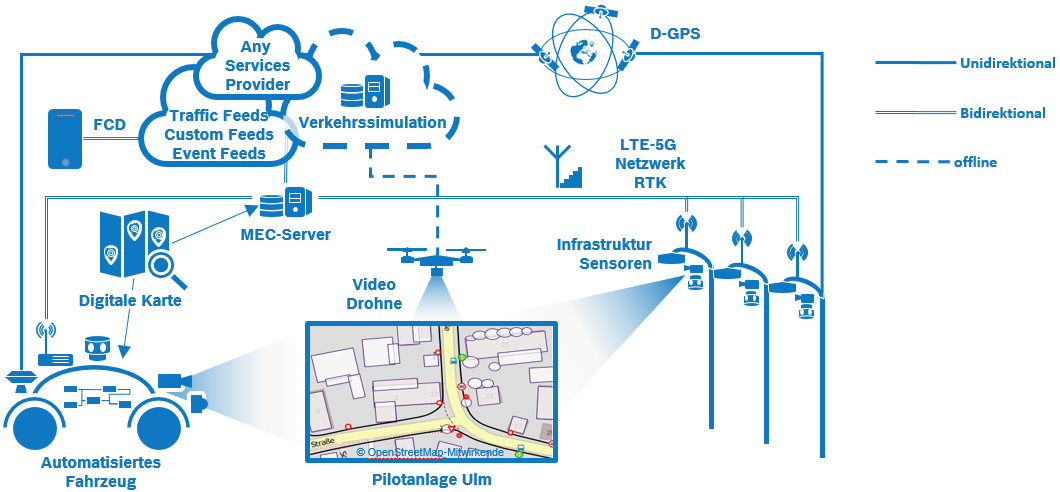
\includegraphics[width=0.7\linewidth]{resources/img/mec_view_arch}
\caption[Überblick MEC-View Projekt]{Überblick MEC-View Projekt \cite[]{mecViewWeb}}
\label{fig:intro_mec_view_arch}
\end{figure}

In urbanen Gebieten
sollen neben Daten von fahrzeuginternen Sensoren auch Informationen externer Infrastruktur-Sensoren verwendet werden,
damit autonome Fahrzeuge eine fundierte Verhaltensentscheidung auf Basis eines detaillierten Umfeldmodells treffen können.
Im Rahmen des Forschungsprojektes MEC-View wird eine Pilot-Anlage zur Umfelderfassung an einer vorfahrtberechtigten Straßenkreuzung
in Ulm aufgebaut und getestet. In dieser Anlage werden die Verkehrsteilnehmer über Kameras und LIDAR-Sensoren erfasst
und die ermittelten Daten über ein schnelles LTE/5G-Mobilfunknetz an einen \textit{Mobile Edge Computing} (\acrshort*{mec}) Server übertragen.
Hier werden die Daten in Echtzeit zu einem Umfeldmodell fusioniert, welches anschließend den autonomen Fahrzeugen
zur besseren Navigation zur Verfügung gestellt wird. Beteiligt an diesem Forschungsprojekt sind neben
der IT-Designers GmbH unter anderem auch die Daimler AG, die Robert Bosch GmbH, Osram, Nokia und die Universität Ulm.
Jeder Projektpartner ist verantwortlich für unterschiedliche Teilaspekte des Projektes. Die IT-Designers GmbH,
bei welcher diese Arbeit angefertigt wird, entwickelt den MEC-Server und ist verantwortlich für das
Teilprojekt \textit{Luftbeobachtung}. \cite[]{mecViewWeb}

\subsection{Das MEC-View Teilprojekt Luftbeobachtung}
\label{sec:mecview_sim}

Im MEC-View Teilprojekt \textit{Luftbeobachtung} werden Verkehrsanalysen und Simulationen erstellt, welche dabei helfen
das Verhalten des Verkehrs besser zu verstehen und es somit ermöglichen, diesen zu optimieren.
Mithilfe der Analysen kann beispielsweise untersucht werden, wie durch die Anpassung von Verkehrssteuerungsanlagen
oder durch die Änderung des Fahrverhaltens einzelner Fahrzeuge, eine Verbesserung der Verkehrssituation erreicht werden kann.
Die Erkenntnisse können insbesondere auch in die Verhaltenssteuerung von autonomen Fahrzeugen mit einfließen.
Aus diesem Grund sind entsprechende Untersuchungen auch für das MEC-View Hauptprojekt relevant.

Die Untersuchungen werden im MEC-View Projekt anhand von Luftbeobachtungen durchgeführt, welche von Drohnen getätigt werden.
In den Videoaufnahmen werden mithilfe eines neuronalen Netzes die Positionen und Fahrzeugklassen der Verkehrsteilnehmer ermittelt.
Mittels dieser kann anschließend beispielsweise die Geschwindigkeit und Beschleunigung der einzelnen Fahrzeuge bestimmt werden.
Zur Erstellung der Analysen ist es zudem wichtig, eine Kenntnis der Topologie der untersuchten Straßen, das heißt des
Verlaufs der Fahrbahnen und Spuren, zu besitzen. In Kombination mit den Fahrzeugpositionen können so interessante
Kenngrößen wie der Verkehrsfluss oder die Verkehrsdichte ermittelt werden.

\section{Motivation und Ziele}
\label{sec:motivation_goals}

Im Rahmen dieser Arbeit wird ein Verfahren zur automatischen Erkennung von Fahrspuren in Luftaufnahmen
auf Basis von Trajektoriedaten entwickelt. Die Spurerkennung wird in die Anwendung \textit{Vehicle-Tracker}
integriert, welche im Rahmen des MEC-View Luftbeobachtungs Projekt erstellt wird. Sie dient der Auswertung
von Luftbeobachtungen des Straßenverkehrs.
In der \textit{Vehicle-Tracker} Applikation mussten bislang die Fahrspurverläufe in jeder Aufnahme
händisch definiert werden. Dieser Prozess ist insbesondere dann aufwendig, wenn die zu untersuchenden
Straßenabschnitte beispielsweise mehrspurige Kreuzungen oder Kreisverkehre beinhalten. Das in dieser Arbeit
entwickelte Spurerkennungs-Modul soll die manuelle Spur-Definition weitestgehend ersetzen und es so ermöglichen
in Zukunft mehr Luftaufnahmen mit weniger Aufwand auszuwerten.

Der Verlauf und die Geometrie der Fahrspuren wird in dieser Thesis anhand der Bewegungsbahnen von Fahrzeugen, den sogenannten Trajektorien,
ermittelt. Im Gegensatz zu einer visuellen Detektierung hat das Verfahren den Vorteil, dass Fahrspuren auch in Aufnahmen
mit schlechten Lichtverhältnissen oder Verdeckungen der Fahrbahnen und Spurmarkierungen erkannt werden können.

Zum Thema Spurerkennung existieren zwar bereits Veröffentlichungen (siehe Abschnitt \ref{sec:rw_lane_detection}),
allerdings können die
vorgestellten Methoden meist nur in sehr speziellen Szenarien eingesetzt werden oder die erkannten Spuren
entsprechen den realen Fahrspurverläufen nur schlecht. Ziel dieser Arbeit ist es, ein Verfahren zu entwickeln,
welches Fahrspuren in möglichst vielen unterschiedlichen Szenarien erkennen kann.
Die Spuren sollen außerdem den realen Fahrbahnverläufen so gut wie möglich entsprechen.

\section{Aufbau dieser Arbeit}
\label{sec:aufbau}

Die vorliegende Arbeit ist wie folgt strukturiert:

\begin{itemize}
    \item Die zum Verständnis der Arbeit und des entwickelten Spurerkennungsalgorithmus benötigten
            Grundlagen sind in \textbf{Kapitel \ref{sec:position_extraction} und \ref{sec:tra_clustering}} beschrieben.
            Kapitel \ref{sec:position_extraction} erläutert, wie aus Luftaufnahmen die Trajektorien von Fahrzeugen
            rekonstruiert und in ein Weltkoordinatensystem überführt werden können.
            Kapitel \ref{sec:tra_clustering} stellt die grundlegenden Konzepte der Clusteranalyse vor, welche
            bei der Umsetzung der Spurerkennung zum Einsatz kommt.
    \item In \textbf{Kapitel \ref{cha:related_work}} werden verwandte Arbeiten, welche sich bereits mit
            der Thematik der Spurerkennung und der Clusteranalyse von Trajektorien befassen, vorgestellt und untersucht.
            Zudem werden Defizite der vorhandenen Lösungen und benötigte Neuerungen aufgezeigt.
    \item In \textbf{Kapitel \ref{cha:konzeption}} wird das Konzept für die Umsetzung der Spurerkennung vorgestellt.
            Es werden Anforderungen definiert und das Spurerkennungs-Modul wird in den Gesamtkontext
            der Applikation \textit{Vehicle-Tracker} eingeordnet.
    \item Nach der Konzeption wird in \textbf{Kapitel \ref{cha:realisation}} erläutert, wie die Spurerkennung in dieser Arbeit
            umgesetzt wurde. Es werden die verschiedenen Schritte des entwickelten Algorithmus vorgestellt.
    \item In \textbf{Kapitel \ref{cha:results}} wird der Spurerkennungsalgorithmus evaluiert.
            Es wird auf die Stärken und Schwächen der wichtigsten Verarbeitungsschritte des Algorithmus eingegangen.
            Außerdem werden konkrete Ergebnisse in Form von Screenshots der erkannten Fahrspuren vorgestellt.
    \item \textbf{Kapitel \ref{cha:end}} bildet den Schluss dieser Masterarbeit. Hier werden die Ergebnisse der
            Arbeit nochmals zusammengefasst und es wird ein Ausblick gegeben, in welchen Anwendungsgebieten die Spurerkennung
            in Zukunft eingesetzt werden kann und welche Verbesserungen an dem entwickelten Verfahren noch vorgenommen werden können.
    \item Im \textbf{\hyperref[cha:anhang_a]{Anhang}} dieser Arbeit sind Aufnahmen der Straßenabschnitte dargestellt,
            mit deren Hilfe der Spurerkennungsalgorithmus entwickelt und evaluiert wurde.
\end{itemize}


%!TEX root = ../Thesis.tex

\chapter{Grundlagen}
\label{cha:grundlagen}

In diesem Kapitel werden die für das Verständnis und die Durchführung der Arbeit benötigten
Grundlagenthemen vorgestellt. Nach einer kurzen Erläuterung der Möglichkeiten der Verkehrsanalysen
mittels Luftaufnahmen, wird daher darauf eingegangen, auf welche Weise die in dieser Arbeit verwendeten
Fahrzeugtrajektorien ermittelt werden.
Anschließend werden Methoden vorgestellt, welche zur Bereinigung der gewonnenen Daten verwendet werden können.
Als wichtiges Mittel zur Identifizierung von Fahrspuren aus Trajektorien werden zudem
verschiedene Cluster-Algorithmen und Distanzmaße vorgestellt.

\section{Verkehrsanalyse mittels Luftaufnahmen}
\label{sec:traffic_analysis}

% Beschreibung der aus den Luftaufnahmen ermittelten (ermittelbaren) Werte
% Vorteile der Verwendung von Luftaufnahmen zur Erstellung von Verkehrssimulationen

\section{Rekonstruktion von Fahrzeugtrajektorien aus Luftaufnahmen}
\label{sec:position_extraction}

% Beschreibung des kompletten Vorgangs bis Bewegungsbahnen der Autos vorliegen
% Tracking --> World-Matching --> initiale Glättung

Die in dieser Arbeit verwendeten Fahrzeugtrajektorien stammen aus der Anwendung ``Tracker-Application''
des MEC-View Teilprojektes \textit{Luftbeobachtung}. Nachfolgend wird beschrieben, wie diese aus den Videoaufnahmen
rekonstruiert werden.

\section{Datenaufbereitung und Bereinigung}
\label{sec:tra_preprocessing}

% ALLGEMEINE Beschreibung von möglichen Datenbereinigungsschritten
% Resampling (Distanz oder Geschwindigkeit)
% Padding etc. (Interpolation)
% Glättung (RANSAC, Wavelet)

\section{Clusteranalyse}
\label{sec:tra_clustering}

Die Clusteranalyse (kurz Clustering) ist ein wichtiges Werkzeug zur Auswertung von Daten unterschiedlichster
Art. Sie stellt dabei kein konkretes Vorgehen oder einen Algorithmus dar, sondern beschreibt ein
allgemeines Problem, welches auf unterschiedlichste Weise gelöst werden kann.
Grundsätzlich ist das Ziel der Clusteranalyse, Datenobjekte aufgrund ihrer Eigenschaften und Beziehungen
untereinander so zu gruppieren, dass sich die Objekte einer Gruppe möglichst stark ähneln und sich
von den Objekten anderer Gruppen möglichst stark unterscheiden. Je höher die \textit{Homogenität} in einem Cluster
und die \textit{Differenz} zwischen den Clustern, desto besser ist die gewählte Clustering Methode.
Der Einsatz von Clustering ist in vielen Anwendungsgebieten und in den unterschiedlichsten wissenschaftlichen
Disziplinen sehr beliebt, um ein Verständnis für Daten zu erhalten beziehungsweise diese anschließend weiter
verarbeiten zu können.
So kommt die Clusteranalyse unter anderem in den Feldern des maschinellen Lernens, der Mustererkennung, Bildanalyse,
der Biologie (Taxonomie) oder im Bereich Data Mining zum Einsatz. \cite[]{tan2007introduction}

Die Clusteranalyse hat viel mit dem Problem der Klassifizierung von Daten gemein, insofern sie Datenobjekten
Label zuordnet. Im Gegensatz zu \textit{überwachten} Klassifizierungsansätzen, wie dem heute populären überwachten
Lernen, leiten Cluster-Algorithmen die Label allerdings alleine aus den vorhandenen Daten ab.
Es kommen keine Vergleichsobjekte mit bekannten, händisch vergebenen Labeln zum Einsatz.
Aus diesem Grund wird die Clusteranalyse auch häufig als \textit{unüberwachte Klassifizierung} bezeichnet. \cite[]{tan2007introduction}

Das Konzept eines \textit{Clusters} ist nicht genau definiert, was in einer Vielzahl an unterschiedlichen Ansichten
und Algorithmen resultiert, welche sich jeweils für andere Anwendungsfälle eignen und verschiedene Eigenschaften
besitzen. Hieraus ergibt sich auch die Tatsache, dass Clustering keine selbsttätiger Prozess ist, welcher sich auf
einheitliche Weise auf unterschiedliche Probleme anwenden lässt. Jedes Problem erfordert die individuelle und sorgfältige
Auswahl eines passenden Algorithmus, eines Distanzmaßes und der richtigen Parameter. Die Bestimmung dieser geschieht
iterativ und nicht selten nach dem Prinzip des \textit{Trial and Error}. In Abbildung \ref{fig:grund_clustering_example}
ist beispielhaft ein Datensatz (links) mit -- für den Menschen intuitiv ersichtlich -- 7 unterschiedlichen Clustern (rechts)
dargestellt. Nach \cite[]{Jain2010} kann allerdings kein verfügbarer Clustering Algorithmus diese alle erkennen.
\cite[]{Jain1999, tan2007introduction}

\begin{figure}[H]
    \centering
    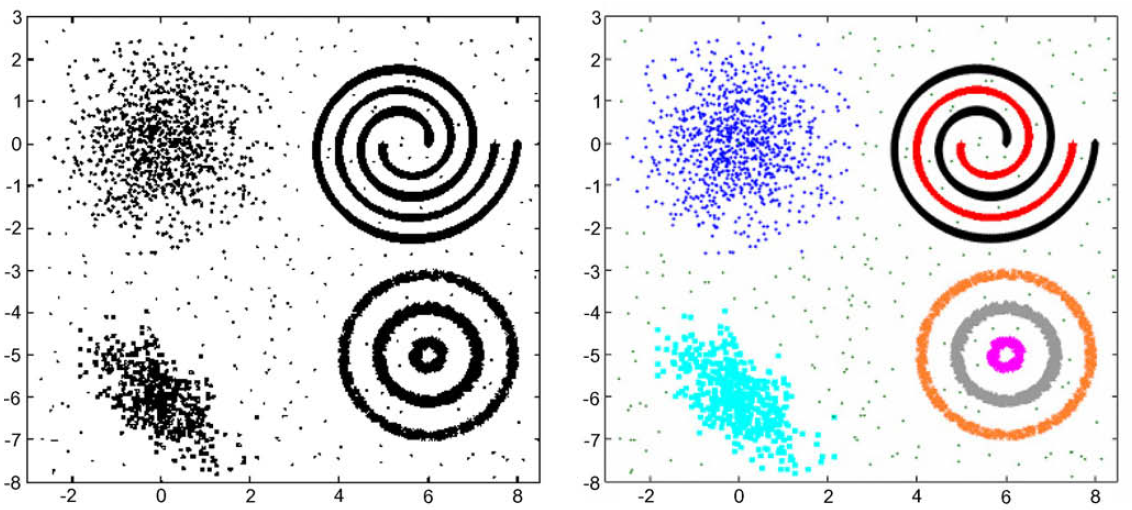
\includegraphics[width=0.8\linewidth]{../resources/img/grundlagen/clustering_example}
    \caption[Rohdaten (links) und erwünschtes Clustering-Ergebnis (rechts)]{Rohdaten (links) und erwünschtes Clustering-Ergebnis (rechts) \cite[]{Jain2010}}
    \label{fig:grund_clustering_example}
\end{figure}

Aufgrund der Limitationen, welche alle Cluster-Algorithmen besitzen, muss der Analyst sich vor deren Anwendung intensiv
mit den zu verarbeitenden Daten beschäftigen. Er muss ein Verständnis dafür besitzen, welche Struktur die Daten
besitzen, beziehungsweise annehmen können, und nach welchen Mustern zu suchen ist.
Besonders wichtiger ist zudem auch die Auswahl der richtigen, das heißt relevanten, Datenmerkmale (\textit{``Feature Selektion''})
und die Wahl deren Repräsentation (\textit{``Feature Transformation''}).
Die Selektion und gegebenenfalls Transformation der Daten muss in einem
Vorverarbeitungsschritt geschehen, dessen Qualität einen maßgeblichen Einfluss auf das finale Clustering Ergebnis hat.
Basierend auf vorangegangener Beschreibung und \cite[]{Jain1999}, lässt sich der Ablauf einer Clusteranalyse wie folgt darstellen:

% TODO: Grafik selbst neu erstellen
% (Feature Selection --> Feature Transformation --> Ähnlichkeitsmessung --> Clustering --> Feedback)
\begin{figure}[H]
    \centering
    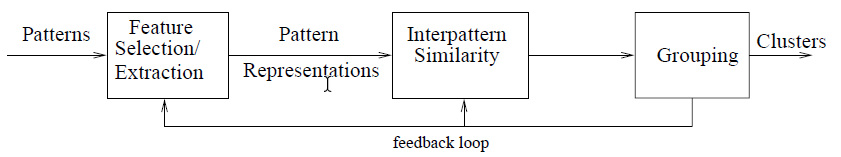
\includegraphics[width=0.8\linewidth]{../resources/img/grundlagen/clustering_workflow}
    \caption{Ablauf einer Clusteranalyse}
    \label{fig:grund_clustering_workflow}
\end{figure}

\cite[]{Jain2010} nennt einige weitere Herausforderungen, welchen man sich bei der Clusteranalyse bewusst sein muss:

\begin{itemize}
    \item Daten können Ausreißer enthalten. Wie sollen diese behandelt werden?
    \item Die Anzahl der Zielcluster ist üblicherweise nicht bekannt.
    \item Validierung der gefundenen Cluster
\end{itemize}

\subsection{Eigenschaften von Cluster-Sets und Clustern}

Das aus einer Analyse resultierende Cluster-Set und die einzelnen Cluster selbst,
können in verschiedene Kategorien unterteilt werden beziehungsweise unterschiedliche Eigenschaften besitzen.
Nachfolgend sind die wichtigsten basierend auf \cite[]{tan2007introduction} und \cite[]{Jain1999,Jain2010} aufgeführt.

\subsubsection{Cluster-Sets}

Bei Cluster-Sets kann grundsätzlich zwischen nachfolgenden Eigenschaften unterschieden werden.

\paragraph{Hierarchisch vs. Partitioniert}
Von \textit{hierarchischen} Cluster-Sets wird gesprochen, wenn die einzelnen Cluster verschachtelt sind und dabei eine
Baum-Struktur bilden. Cluster sind hingegen \textit{partitioniert}, wenn keine Überlagerungen zwischen ihnen existiert.

\paragraph{Exklusiv vs. Überlappend vs. Fuzzy}
\textit{Exklusive} Cluster-Sets liegen vor, wenn jedem Datenwert ein oder kein Zielcluster zugeordnet wird.
Im Gegensatz hierzu können bei \textit{überlappenden} Cluster-Sets Objekte einer oder mehrerer Gruppen angehören.
Bei dem sogenannten \textit{Fuzzy} oder \textit{Soft} Cluster-Sets, gehört ein Datenobjekt einem Cluster
mit einer bestimmten Wahrscheinlichkeit oder Gewicht an. Algorithmen, welche Daten eine
Wahrscheinlichkeit für die Zugehörigkeit zu einem Cluster zuweisen, werden \textit{probabilistische}
Cluster-Algorithmen genannt.

\paragraph{Komplett vs. Partielle}
Von \textit{kompletten} Cluster-Sets wird gesprochen, wenn jedes Element der Eingangsdaten einem Cluster zugeordnet wird.
Bei \textit{partiellen} Sets ist dies nicht der Fall. Hier kann ein bestimmter Anteil an Datenwerten als Ausreißer markiert
werden, welche keine Gruppe besitzen.

% TODO: evtl. Bild einfügen

\subsubsection{Cluster}

Da, wie oben erwähnt, nicht klar definiert ist, was ein Cluster ausmacht, können auch diese unterschiedliche Eigenschaften
besitzen. Die wichtigsten Cluster-Arten sind nachfolgend erläutert.

\paragraph{Klar separierte Cluster}
Unter \textit{klar separiereten} Clustern versteht man solche, in welchen jedes Datenelement einen geringeren
Abstand zu allen anderen Elementen des Clusters hat, als zu Elementen außerhalb des Clusters. Diese
idealistische Definition eines Clusters ist nur dann erfüllt, wenn die in den Daten enthaltenen Cluster einen
großen Abstand voneinander haben. Dies ist in der Realität allerdings selten der Fall.

\paragraph{Prototyp basierte Cluster}
Von einem \textit{Prototyp basierten} Cluster wird gesprochen, wenn alle Elemente einer Gruppe einen
geringeren Abstand zu einem Prototyp oder Referenzwert des Clusters besitzen, als zu denen anderer Gruppierungen.
Ein solcher Prototyp ist üblicherweise der Mittelwert der Datenelemente eines Clusters (\textit{Centroid}).

\paragraph{Graphen basierte Cluster}
Die Definition eines \textit{Graphen basierten} Clusters kann immer dann verwendet werden, wenn Daten
als vernetzter Graph dargestellt werden. In einem solchen sind die Elemente Knoten und die Kanten
repräsentieren Beziehungen zwischen ihnen. Ein Cluster in einem solchen Graphen ist definiert als Menge von
Knoten, welche untereinander verbunden sind, jedoch keine Verbindungen zu Elementen außerhalb des Clusters haben.

\paragraph{Dichte basierte Cluster}
\textit{Dichte basierte} Cluster sind definiert als Regionen mit einer hohen Dichte an Objekten, welche von
Regionen umgeben sind, welche eine geringe Objektdichte besitzen. Elemente, welche in einer solchen Region
mit geringen Dichte liegen, welche aus Ausreißer interpretiert. Dichte Bereiche werden üblicherweise
gefunden, indem die Nachbarschaften von Elementen untersucht werden.

\paragraph{Konzeptionelle Cluster}
% TODO: Verweis Bild hinzufügen
Eine sehr allgemeine Definition eines Clusters ist die der \textit{konzeptionellen} Gruppen. Hiermit ist
gemeint, dass die Elemente eines Clusters einige gemeinsame Eigenschaften besitzen. Dies schließt die oben genannten
Cluster-Arten mit ein, lässt sich allerdings beliebig erweitern. So sind beispielsweise in Abbildung XXX x)
konzeptionelle Cluster dargestellt, die die Form zweier Kreise und eines Dreiecks haben. Um solche Muster
erkennen zu können, würde ein Algorithmus eine besondere Definition eines Clusters benötigen.


% TODO: Bild hinzufügen und referenzieren

\subsection{Cluster-Algorithmen}
\label{sec:cluster_algos}

Um mit den oben beschriebenen unterschiedlichen Cluster-Set und Cluster Definitionen umgehen zu können,
existieren verschiedene Clustering-Modelle.
Einige wichtige Clustering-Ansätze sind die Vernetzungs-Modelle, Centroid-basierte-Modelle, Verteilungs-Modelle
oder Dichte-Modelle. Für jedes dieser Modelle existieren unterschiedliche Algorithmen. Im Folgenden werden
diese Modelle und jeweils exemplarisch ein Algorithmus der diese vertritt vorgestellt.

\subsubsection{Vernetzungs-Modelle}

Vernetzungs-Modelle werden auch häufig \textit{hierarchische Cluster-Modelle} genannt. Sie beruhen auf
der Annahme, dass Elemente, welche nahe beieinander liegen, eine höhere Gemeinsamkeit besitzen als solche,
welche weiter voneinander entfernt sind. Zur Bestimmung der Nähe zwischen Elementen benötigen Vernetzungs-Modelle,
wie auch andere Cluster-Modelle, eine
Definition von Distanz. Diese legt ein sogenanntes \textit{Distanzmaß} fest. Zusätzlich ist ein \textit{Link-Kriterium} notwendig,
welches bestimmt, wie genau die Entfernung zwischen zwei Clustern ermittelt wird. Übliche Link-Kriterien
sind \textit{Minimum-Linkage}, welches die minimale Distanz zwischen den Objekten der Cluster als Distanz verwendet,
oder \textit{Maximum-Linkage} beziehungsweise \textit{Average-Linkage}. \cite[]{Jain1999, GeorgeSeif2018}

Grundsätzlich teilen sich hierarchische Cluster-Algorithmen in zwei Gruppen auf:
\textit{Agglomerative} (Bottom-Up) und \textit{Divisive} (Top-Down) Algorithmen.
Agglomerative Ansätze weisen zu Beginn des Cluster-Vorgangs jedem Datenelement eine eigene Gruppe zu und vereinigen
diese anschließend.
Bei divisiven Ansätzen werden hingegen zu Beginn alle Elemente in einem Cluster zusammengefasst und
diese in den nachfolgenden Schritten geteilt.

Als Beispiel wird anschließend der \textbf{agglomerative-hierarchische Cluster-Algorithmus} genauer vorgestellt.
Sein Vorgehen lässt sich sehr gut anhand sogenannter Dendrogramme oder geschachtelter Cluster-Diagramme darstellen
(siehe Abbildung \ref{fig:grund_agglo_clustering})

% TODO: Bild selbst erstellen
\begin{figure}[H]
    \centering
    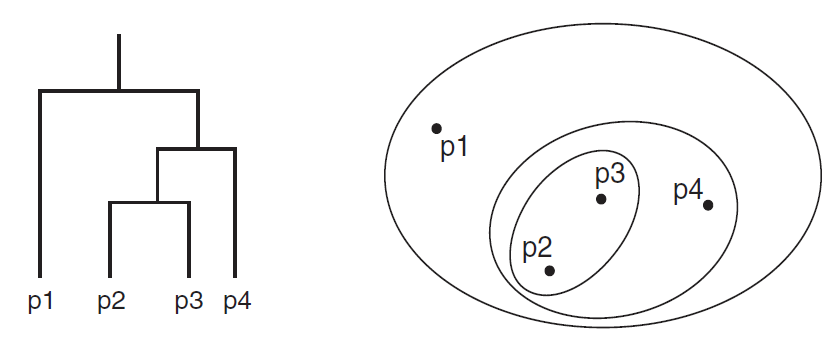
\includegraphics[width=0.7\linewidth]{../resources/img/grundlagen/agglo_clustering}
    \caption{Agglomeratives Clustering dargestellt als Dendrogramm und geschachteltes Cluster-Diagram}
    \label{fig:grund_agglo_clustering}
\end{figure}

Im ersten Schritt des Algorithmus werden alle Datenpunkte als separate Cluster markiert. Diesen Schritt
repräsentieren die Blätter des Dendrogramms.
Anschließend muss ein Distanzmaß und ein Link-Kriterium gewählt werden.
Das am häufigsten verwendete Distanzmaß ist sicherlich der euklidsche Abstand, welcher die Distanz zwischen zwei Punkten
oder Vektoren im $n$-dimensionalen Raum bestimmt. Er ist definiert durch die Formel \ref{eq_dist}.

\begin{ceqn}
\begin{align}
\label{eq_dist}
    dist(p,q) = ||q-p||_2 = \sqrt{\sum_{i=1}^n (q_i-p_i)^2}
\end{align}
\end{ceqn}

Wird als Link-Kriterium beispielsweise \textit{Minimum-Linkage} gewählt, ist dieses definiert als:

\begin{ceqn}
\begin{align}
\label{eq_linkage}
    link(P, Q) = min\{ dist(p,q) : p \in P, q \in Q\}
\end{align}
\end{ceqn}

Hierbei entsprechen $P$ und $Q$ zwei Clustern, welche die Elemente $p \in P$ und $q \in Q$ enthalten.
Auf Basis des gewählten Link-Kriteriums kann nun eine Distanz-Matrix für die einzelnen Cluster
erstellt werden.
Die zwei Cluster mit minimalem Abstand voneinander werden anschließend zusammengeführt und die
vorherigen Schritte werden wiederholt, bis nur noch ein Cluster (Wurzel des Dendrogramms) beziehungsweise
die gewünschte Clusteranzahl übrig ist. \cite[]{GeorgeSeif2018, tan2007introduction}

Bei den meisten Varianten des agglomerativen Clusterings muss der Nutzer die Anzahl der Zielcluster im
vorraus festlegen, was problematisch ist, da diese meist nicht bekannt ist. Umgangen werden kann dies nur,
indem ein Link-Kriterium gewählt wird, das ab einer bestimmten Distanz zwischen den Clustern diese nichtmehr
fusioniert \cite[]{GeorgeSeif2018}.

Die Zeitkomplexität des agglomerativen Clusterings beträgt bestenfalls $O(m^2log\ m)$, weshalb die Menge der Daten,
welche mit ihm verarbeitet werden können erheblich begrenzt ist \cite[]{tan2007introduction}.

\subsubsection{Centroid-Modelle}

Centroid basierte Cluster-Modelle betrachten im Gegensatz zu hierarchischen Modellen nicht die Distanz
zwischen Clustern, sondern die Entfernung von Objekten zu Referenzpunkten, sogenannten \textit{Centroids}.

Ein Beispiel für einen Centroid-Cluster-Algorithmus ist \textbf{k-Means}. Dieser ist aufgrund seines Alters,
seiner Einfachheit und der vielen Weiterentwicklungen wohl der bekannteste Cluster-Algorithmus überhaupt.

Das Ziel von k-Mean ist es, für eine n-dimensionale Punktmenge $X = \{ x_1 ... x_n \}$ ein Cluster-Set $C = \{ c_1 ... c_k \}$
zu finden, welches die Summe der quadratischen Abweichung (Gleichung \ref{eq_kmeans1}) zwischen allein Punkten in einem Cluster und deren
Mittelwert $\mu_k$ (Centroids) minimiert.

\begin{ceqn}
\begin{align}
    \label{eq_kmeans1}
    J(c_k) = \sum_{k=1}^K \sum_{x_i \in c_k} || x_i - \mu_k ||^2
\end{align}
\end{ceqn}

Eine Lösung für dieses Problem zu finden, ist NP-Schwer. Aus diesem Grund
ist k-Means ein approximativer Ansatz, welcher nicht garantieren kann, ein globales Minimum zu finden.
Die Funktionsweise des Algorithmus ist in Abbildung \ref{fig:grund_kmeans_clustering} dargestellt.
Die Kreuze entsprechen hierbei den Centroids, welche sich über die Iterationen hinweg verschieben.

\begin{figure}[H]
    \centering
    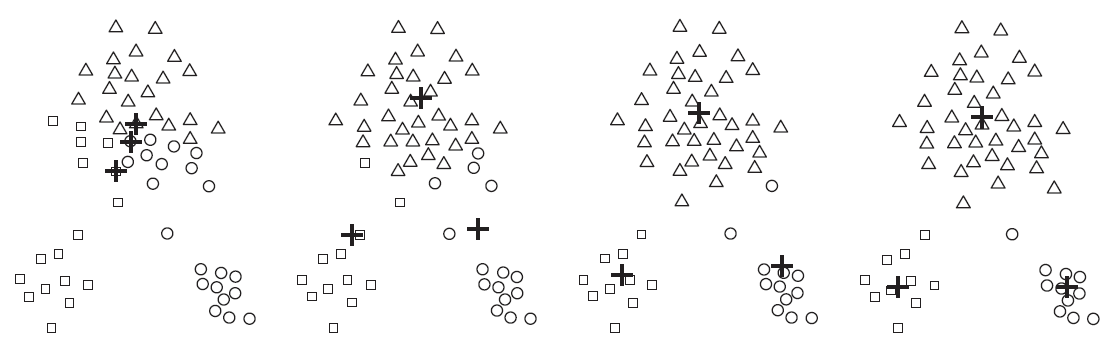
\includegraphics[width=0.9\linewidth]{../resources/img/grundlagen/k-means}
    \caption[Funktionsweise von k-Means]{Funktionsweise von k-Means \cite[]{tan2007introduction}}
    \label{fig:grund_kmeans_clustering}
\end{figure}

Ausgehend von der Punktmenge $X$ und der gesuchten Cluster-Anzahl $k$,
werden im ersten Schritt $k$ zufällig positionierte Centroids $\mu_k$ definiert.
Anschließend wird für alle Punkte $x_i$ der nächstgelegene Centroid $\mu_j$ gesucht.

\begin{ceqn}
\begin{align}
    \label{eq_kmeans2}
    j = arg\ min(dist(x_i, \mu_j))
\end{align}
\end{ceqn}

$x_i$ wird daraufhin Mitglied in Cluster $C_j$. Als Distanzmaß ($dist$) kann hier wieder der euklidsche Abstand
(Gleichung \ref{eq_dist}) verwendet werden oder aber auch beliebige andere sinnvolle Metriken.
Nachdem alle Punkte $x_i$ einem Cluster zugewiesen wurden, werden die Centroid Positionen neu bestimmt.
Hierzu wird der Durchschnitt aller Punkte eines Clusters berechnet:

\begin{ceqn}
\begin{align}
    \label{eq_kmeans3}
    c_j = \frac{1}{n} \sum_{x_j \in C_j} x_j
\end{align}
\end{ceqn}

Diese zwei Schritte werden mehrfach wiederholt, bis das Ergebnis konvergiert, das heißt die Zuweisungen sich
nurnoch geringfügig ändern. \cite[]{Jain2010}

Der primäre Nachteil des k-Means Algorithmus ist, das auch bei ihm die Anzahl der Zielcluster spezifiziert
werden muss. Desweiteren ist sein Ergebnis aufgrund der zufälligen Initialisierung der Centroids
nicht deterministisch. Vorteil von k-Means ist hingegen, dass seine Zeitkomplexität bei $O(n)$ liegt.

Um die genannten Nachteile, zumindest in Teilen, umgehen zu können, existieren diverse Weiterentwicklungen des k-Mean
Algorithmus. So stammen beispielsweise von \cite[]{Hamerly} und \cite[]{Pelleg} die Algorithmen \textit{g-Means}
beziehungsweise \textit{x-Means}, welche die Clusteranzahl $k$ auf Basis mehrerer k-Means Durchläufe und
statistischer Kennzahlen bestimmen.

\subsubsection{Distributions-Modelle}

Distributions-Cluster-Modelle basieren auf der Verwendung von statistischen Wahrscheinlichkeitsverteilungen wie
beispielsweise der Gauß-Verteilung. Cluster werden darüber definiert, wie wahrscheinlich es ist, dass Objekte
der selben Verteilung angehören. Problematisch ist die Verwendung dieser Cluster-Methodik, da sie anfällig für
das Problem des \textit{``Overfitting''} ist, wenn die Komplexität der verwendeten Modelle nicht beschränkt wird.
Zudem ist die Annahme, dass vielen realen Datensätzen ein statistisches Verteilungsmodell zugrundeliegt, gefährlich.
Ist diese These jedoch berechtigt, haben die Modelle den Vorteil, dass sie neben der Zuweisung von Objekten zu Clustern
auch Korrelationen zwischen einzelnen Attributen aufzeigen können. \cite[]{AndersDrachen2014}

Nachfolgend wird der bekannteste Vertreter der Distributions-Cluster-Algorithmen vorgestellt:
das \textit{Expectation–maximization} (EM) Verfahren unter Verwendung sogenannter \textit{Gaussian-Mixture-Models} (GMM).
Die Funktionsweise des EM-Algorithmus hat grundsätzlich viel gemein mit der des k-Mean Ansatzes.
Es wird ebenfalls mit einer festen Anzahl zufällig initialisierter Modelle gestartet, welche anschließend über mehrere Iterationen
an die Daten angepasst werden. Im Gegensatz zu k-Means, sind die gewählten Modelle hingegen Gauß-Verteilungen,
welche zwei Parameter besitzen: ihren Mittelwert und die Standardabweichung.
Das Vorgehen des EM-Algorithmus ist nachfolgend, basierend auf \cite[]{GeorgeSeif2018}, beschrieben und in
Abbildung \ref{fig:grund_em_clustering} grafisch dargestellt.

\begin{description}
    \item[1)] Wahl der Clusteranzahl $k$ und Initialisierung der Gauß-Modelle für die entsprechenden Cluster.
    \item[2)] Berechnung der Wahrscheinlichkeit, dass ein Datenpunkt zu einem Cluster gehört. Je näher
              ein Datenpunkt dem Zentrum einer Gauß-Verteilung ist, desto höher die Wahrscheinlichkeit für dessen Zugehörigkeit.
    \item[3)] Basierend auf den Wahrscheinlichkeiten werden die Parameter der Verteilungen neu berechnet.
              Hierzu wird die gewichtete Summe der Datenpunkt-Positionen errechnet. Die Gewichte entsprechen dabei
              den Wahrscheinlichkeiten, dass ein Element zu einem Cluster gehört. Hierdurch werden die Gauß-Modelle automatisch
              den in den Daten enthaltenen Clustern angepasst.
    \item[4)] Wiederholdung der Schritte 2) und 3), bis das Clustering-Ergebnis konvergiert.
\end{description}

\begin{figure}[H]
    \centering
    \subfloat[Iteration 1]{{
        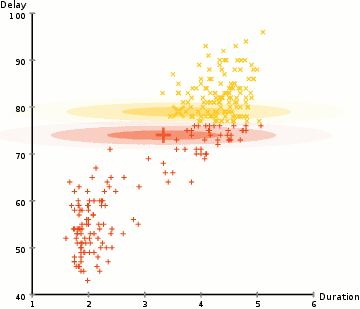
\includegraphics[width=0.22\linewidth]{../resources/img/grundlagen/clustering_EM/EM1}
    }}
    \subfloat[Iteration 2]{{
        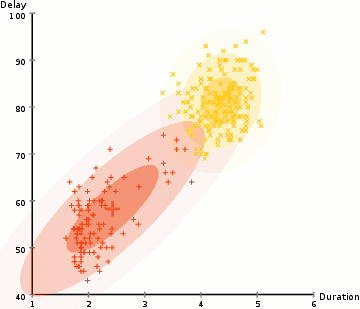
\includegraphics[width=0.22\linewidth]{../resources/img/grundlagen/clustering_EM/EM2}
    }}
    \subfloat[Iteration 3]{{
        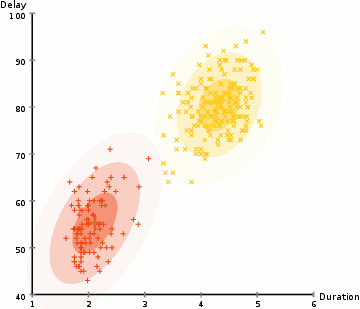
\includegraphics[width=0.22\linewidth]{../resources/img/grundlagen/clustering_EM/EM3}
    }}
    \subfloat[Iteration 4]{{
        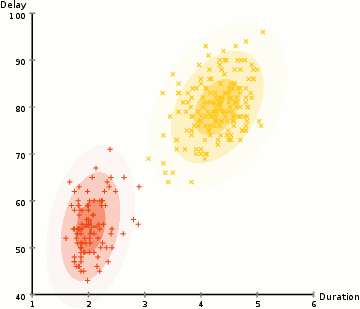
\includegraphics[width=0.22\linewidth]{../resources/img/grundlagen/clustering_EM/EM4}
    }}
    \caption[Darstellung des EM-Cluster-Algorithmus über mehrere Iterationen]{Darstellung des EM-Cluster-Algorithmus über mehrere Iterationen \cite[]{GeorgeSeif2018}}
    \label{fig:grund_em_clustering}
\end{figure}

Ziel des EM-Algorithmus ist es, die Parameter der Gauß-Modelle so zu optimieren, dass diese die Verteilung der Daten bestmöglich beschreiben.
Am Ende des Clusterings besitzt jeder Datenwert die Zugehörigkeit-Wahrscheinlichkeiten für die einzelnen Cluster.
Ein Element wird jenem Cluster zugeordnet, für welches es die höchste Wahrscheinlichkeit besitzt.

\subsubsection{Dichte-Modelle}

Dichte basierte Cluster sind, wie oben beschrieben, definiert als Regionen hoher Objekt-Dichte, welche
von Bereichen geringer Dichte umgeben sind. Dichte-Clustering-Modelle suchen nach eben solchen Regionen.
Großer Vorteil der Algorithmen dieser Klasse ist, dass sie Cluster beliebiger Formen finden können,
nicht auf die Vorgabe einer Clusteranzahl angewiesen sind und mit Ausreißern umgehen können.

Als Vertreter der Dichte-basierten Ansätze wird nachfolgend der \textbf{DBSCAN} Algorithmus
(\textit{Density-Based Spatial Clustering of Applications with Noise}), wie in \cite[]{Gao2012} beschrieben, vorgestellt.
Er verwendet als Maß für die Dichte einer Region die sogenannte \textit{$\epsilon$ -Nachbarschaft} (\textit{Eps}).
Diese selektiert für ein Objekt $p$ alle Objekte, welche innerhalb des Radius $\epsilon$ um dieses liegen:

\begin{ceqn}
\begin{align}
    \label{eq_dbscan_1}
    N_{\epsilon}(p) = \{ q | dist(p,q) \leq \epsilon \}
\end{align}
\end{ceqn}

Eine $\epsilon$ -Nachbarschaft besitzt eine hohe Dichte, wenn in ihr mindestens $MinPts$ Objekte liegen.

Basierend auf der Definition von \textit{Eps}, werden die in einem Datensatz vorhandenen Elemente in
drei Klassen unterteilt. Sie sind entweder \textit{Kern-}, \textit{Rand-} oder \textit{Ausreißer-} Objekte.
Ein Kernobjekt hat mindestens $MinPts$ andere Punkte in \textit{Eps}.  
Randobjekte besitzen weniger als $MinPts$ in \textit{Eps}, liegen aber in der Nachbarschaft eines Kernobjektes.
Ausreißerobjekte sind weder Kern- noch Randobjekte.

\begin{figure}[H]
    \centering
    \subfloat[]{{
        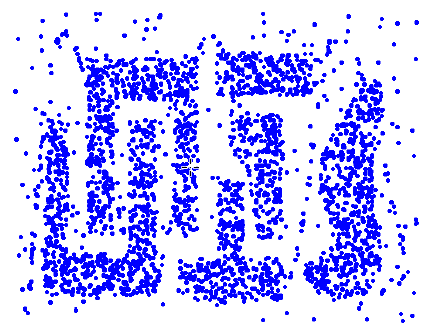
\includegraphics[width=0.3\linewidth]{../resources/img/grundlagen/clustering_dbscan/dbscan1}
    }}
    \subfloat[]{{
        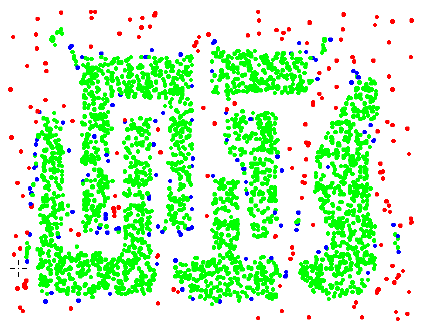
\includegraphics[width=0.3\linewidth]{../resources/img/grundlagen/clustering_dbscan/dbscan2}
    }}
    \subfloat[]{{
        
\includegraphics[width=0.3\linewidth]{../resources/img/grundlagen/clustering_dbscan/dbscan3}
    }}
    \caption[Schritte des DBSCAN Algorithmus]{Schritte des DBSCAN Algorithmus, a) Rohdaten, b) Klassifizierung in Kern- (grün), Rand- (blau) und Ausreißer- (rot) Punkte, c) Cluster Ergebnis \cite[]{Gao2012}}
    \label{fig:grund_dbscan_clustering}
\end{figure}

Auf Basis der drei Objektklassen, lässt sich das Prinzip der dichte-basierten \textit{Erreichbarkeit} definieren.
Ein Objekt $q$ ist von $p$ \textit{direkt} erreichbar, wenn $p$ ein Kernobjekt ist und $q$ in dessen \textit{Eps} liegt.
In Abbildung \ref{fig:grund_dbscan_reachability} gilt dies beispielsweise für $p$ und $p_2$.
Zwei Elemente sind \textit{indirekt} erreichbar, wenn sie über eine Reihe von Zwischenschritten (direkte Relationen)
verbunden sind (transitiv). Dies ist in Abbildung \ref{fig:grund_dbscan_reachability} für $q$ und $p$ der Fall.

\begin{figure}[H]
    \centering
    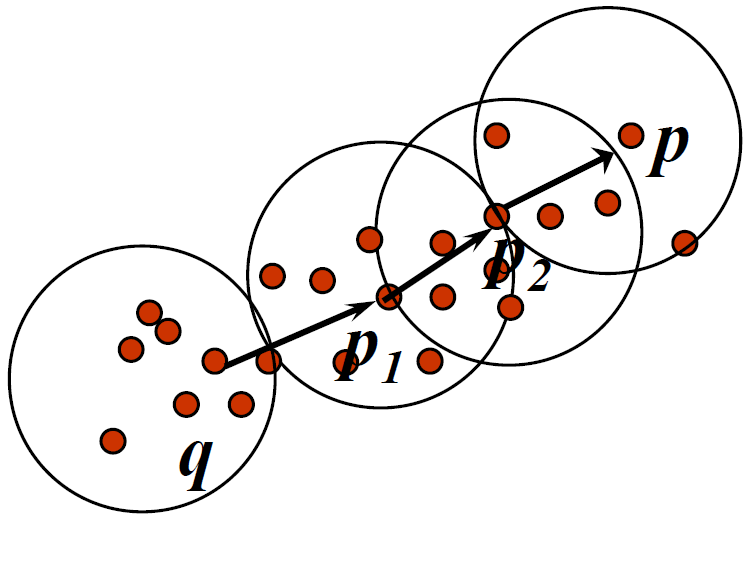
\includegraphics[width=0.32\linewidth]{../resources/img/grundlagen/clustering_dbscan/reachability}
    \caption[Erreichbarkeit in DBSCAN]{Erreichbarkeit in DBSCAN \cite[]{Gao2012}}
    \label{fig:grund_dbscan_reachability}
\end{figure}

Der DBSCAN Algorithmus lässt sich, basierend auf den obigen Definitionen, informell wie folgt beschreiben:

\begin{description}
    \item[1)] Unterteilung der Objekte in die drei Objektklassen. (Abb. \ref{fig:grund_dbscan_clustering} b))
    \item[2)] Aussortierung der Ausreißer-Objekte.
    \item[3)] Wahl eines nicht zugewiesenen Kernobjektes.
    \item[4)] Erstellung eines neuen Clusters für das Kernobjekt und alle von ihm ausgehend direkt oder indirekt erreichbaren Objekte
    \item[5)] Wiederholdung der Schritte 3) und 4), bis alle Kern- und Randobjekte einem Cluster zugewiesen sind. (Abb. \ref{fig:grund_dbscan_clustering} c))
\end{description}

DBSCAN besitzt die oben beschriebenen Vorteile Dichte-basierter Cluster-Algorithmen. Dank einer Zeitkomplexität
von $O(n\ log\ n)$ kann er außerdem auch auf große Datensätze angewendet werden.
Nachteil des Ansatzes ist hingegen, dass er schlecht mit Clustern umgehen kann, welche unterschiedliche Dichten besitzen. 

\section{Ähnlichkeitsmaße zum Vergleich von Fahrzeugtrajektorien}
\label{sec:distance_measures}

Bei der Clusteranalyse ist neben der Wahl des passenden Cluster-Algorithmus insbesondere
die Entscheidung, welches Ähnlichkeits- beziehungsweise Distanzmaß verwendet wird, ausschlaggebend.
Im obigen Abschnitt wurden bereits die euklidsche Distanz (Gleichung \ref{eq_dist}) als ein mögliches Distanzmaß
definiert. Dieses kann jedoch nur zur Bestimmung der Distanz zwischen $n$-dimensionalen Punkten im euklidschen Raum verwendet
werden. Dies gilt ebenso für andere einfache Maße wie die Manhatten-Distanz oder die Pearson-Distanz.

Um Fahrzeugtrajektorien korrekt gruppieren zu können, ist ein Ähnlichkeitsmaß notwendig, welches je nach Anforderungen
die unterschiedlichen Aspekte der Trajektorien vergleicht. Häufig werden die Eigenschaften Lage, Form und Länge
hierzu herangezogen. In der Literatur werden diverse Maße zum Vergleich von Trajektorien vorgestellt. Diese besitzen
alle unterschiedliche Eigenschaften, Vor- und Nachteile.

Nachfolgend werden exemplarisch drei Ähnlichkeitsmaße vorgestellt, anhand welcher ersichtlich ist, welche Abwägungen
bei der Wahl des Maßes gemacht werden müssen.
In allen drei Fällen werden die Trajektorien als Reihen 2-dimensionaler Punkte mit Länge $n$ interpretiert: $t_i = \{(x_1, y_1), (x_2, y_2), ..., (x_n, y_n)\}$.
Der $n$-te Punkt einer Trajektorie ist gegeben über $t_i(n)$ und deren Punkt-Länge über $len(t_i)$.
Die Menge der zu vergleichenden Trajektorien ist $T = \{t_1, t_2, ..., t_m\}$.
Abbildung \ref{fig:grund_trajectories} zeigt eine Auswahl möglicher Trajektorien.

\begin{figure}[H]
\centering
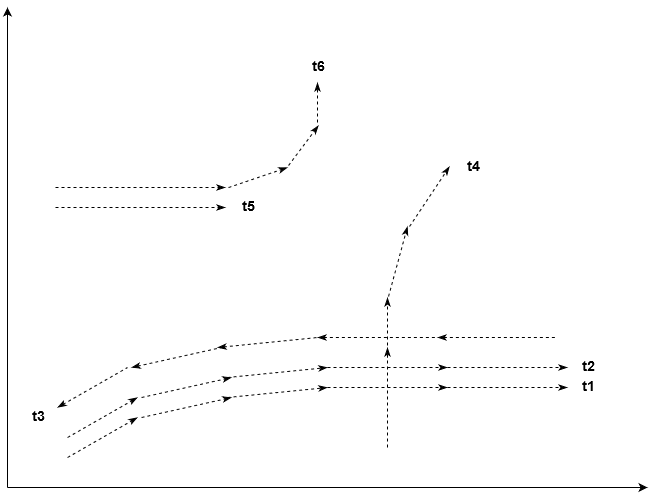
\includegraphics[width=0.6\linewidth]{../resources/img/grundlagen/trajectories}
\caption{Trajektorien im 2-dimensionalen Raum}
\label{fig:grund_trajectories}
\end{figure}

\subsection{HU Distanz}

Die HU Distanz wurde erstmals in der Arbeit \textit{``Similarity based vehicle trajectory clustering and anomaly detection''}
von \cite[]{Hu2005} verwendet. Es ist ein sehr einfaches Distanzmaß, welches auf der mittleren euklidschen Distanz
zwischen zwei Trajektorien basiert. Berechnet wird die HU Distanz für zwei Trajektorien $t_1$ und $t_2$ wie folgt:

\begin{ceqn}
\begin{align}
\label{eq_hu_distance1}
    D_{HU}(t_1, t_2) &= \frac{1}{N} \sum_{n = 1}^N dist(t_1(n), t_2(n)) \\
\label{eq_hu_distance2}
    wobei\ N &= min(len(t_1), len(t_2))
\end{align}
\end{ceqn}

Aus dieser Formel lassen sich die Vor- und Nachteile der HU Distanz ableiten. Der klare Vorteile der
HU Distanz ist deren Einfachheit und die Effizienz von $O(n)$.
Nachteil ist hingegen, dass das Distanzmaß nur gut funktioniert, wenn die Trajektorien bestimmte
Kriterien erfüllen. So sollten Trajektorien, welche einem Cluster angehören, auch immer möglichst auf selber Höhe beginnen,
damit deren mittlerer Abstand nicht, aufgrund einer Verschiebung, erhöht wird.
Außerdem ist es notwendig, die Abstände zwischen den Punkten der Trajektorien auf die selbe Länge zu bringen,
damit beim paarweisen Vergleich immer Elemente verglichen werden, welche gleichweit vom Start der Spuren entfernt sind. 
Diese Eigenschaften der Trajektorien müssen über einen Vorverarbeitungsschritt geschaffen werden. 
Problematisch bei der Verwendung der HU Distanz ist außerdem, dass beim Vergleich zweier Trajektorien immer nur
die ersten $N$ Punkte (s. Gleichung \ref{eq_hu_distance2}) betrachtet werden. Die kann dazu führen, dass zwei
Trajektorien, welche zu Beginn fast identisch sind und später auseinanderlaufen, trotzdem einen hohen Ähnlichkeitswert besitzen
(siehe $t_5$ und $t_6$ in Abbildung \ref{fig:grund_trajectories}).

Die HU Distanz kann aufgrund der genannten Einschränken nur in speziellen Fällen oder unter Verwendung eines
Vorverarbeitungsschrittes angewandt werden. Sie liefert ansonsten suboptimale Clustering Ergebnisse.

\subsection{Hausdorff Distanz}

Die Hausdorff Distanz ist ein komplexeres Maß zur Bestimmung der Ähnlichkeit zwischen zwei Trajektorien.
Sie misst grundsätzlich den Abstand zwischen zwei nicht-leeren, ungeordneten Teilmengen $A$ und $B$ und ist für
Trajektorien definiert über die Gleichungen \cite[]{Atev2010}:

\begin{ceqn}
\begin{align}
\label{eq_hausdorff1}
    D_{HD}(t_1, t_2) &= max(h(t_1, t_2), h(t_2, t_1)) \\
\label{eq_hausdorff2}
    h(t_1, t_2) &= \underset{i\ \in\ t_1}{max}\ \underset{j\ \in\ t_2}{min}\ dist(i, j)
\end{align}
\end{ceqn}

$h(t_1, t_2)$ wird als gerichtete Hausdorff Distanz \textit{von} $t_1$ \textit{nach} $t_2$ bezeichnet.
Sie findet die maximale Distanz einer Trajektorie zum nächsten Punkt der anderen Trajektorie \cite[]{Huttenlocher}.
Da $h$ gerichtet ist, gilt $h(t_1, t_2) \neq h(t_2, t_1)$. Aus diesem Grund wird die Hausdorff Distanz
\textit{zwischen} zwei Trajektorien mittels $D_{HD}$ bestimmt. $dist$ kann ein beliebiges Maß für die Distanz zweier
Punkte sein, wie beispielsweise die euklidsche Distanz.
Grundsätzlich lässt sich über die Hausdorff Distanz die Form zweier Trajektorien vergleichen. Diese sind ähnlich,
wenn jeder Punkt einer Trajektorie einen nahegelegenen Punkt in der Vergleichsbahn besitzt.

Vorteil der Hausdorff Distanz im Vergleich zur HU Distanz ist, dass diese immer vollständige Trajektorien vergleicht
und nicht nur Teile. Außerdem ist bei ihrer Verwendung keine Vorverarbeitung in Form von Resampling et cetera notwendig.
Problematisch ist das Distanzmaß hingegen, da es mit ungeordneten Sets arbeitet und somit im Fall von Trajektorien deren
Orientierung nicht beachtet. Zwei parallel aber in entgegengesetzte Richtungen laufende Trajektorien würden
nach Hausdorff daher eine hohe Ähnlichkeit besitzen.
Zudem kann das Distanzmaß schlecht mit Ausreißern umgehen, da bereits ein einzelner dieser Punkte, bei ansonsten identischen
Trajektorien, zu einer beliebig kleinen Ähnlichkeit führen kann.
Von Nachteil ist auch, dass die Zeitkomplexität der Hausdorff-Distanz bei $O(n\ m)$ liegt.

\subsection{Longest-Common-Subsequence}

Das \textit{Longest-Common-Subsequence} (LCSS) Ähnlichkeitsmaß basiert auf dem allgemeinen Problem der Findung
einer längsten gemeinsamen Subsequenz zwischen zwei Sequenzen. Da Trajektorien, nach obiger Definition, lediglich Punktfolgen sind,
lässt sich das Verfahren sehr gut auf diese anwenden. Aufgrund einiger kleiner Erweiterungen des Basis-Algorithmus, besitzt
das LCSS Ähnlichkeitsmaß einige besondere Eigenschaften. Der LCSS Algorithmus für Trajektorien ist grundsätzlich
wie folgt definiert \cite[]{Vlachos}:

\begin{ceqn}
\begin{align}
\label{eq_lcss}
    LCSS_{\epsilon, \delta}(t_1, t_2) =
    \begin{cases}
        0 & \text{if } t_1 \text{ or } t_2 \in \emptyset \\
        1 + LCSS_{\epsilon, \delta}(t_1', t_2') & \text{if } dist(t_1(n), t_2(m)) < \epsilon \\
        & \land\ |n - m| \leq \delta \\
        max(LCSS_{\epsilon, \delta}(t_1', t_2), LCSS_{\epsilon, \delta}(t_1, t_2')) & \text{otherwise}
    \end{cases}
\end{align}
\end{ceqn}

Hierbei gilt $t_1' = \{ t_1(0),\ ...,\ t_1(n-1)\}$. Die Parameter $\epsilon$ und $\delta$ bestimmen das
Vergleichs-Verhalten des Algorithmus. Über $\epsilon$ wird definiert, wieweit zwei Punkte maximal voneinander entfernt liegen
können, um immer noch als ``übereinstimmend'' zu gelten. $\delta$ bestimmt hingegen, wieweit man in der Zeit gehen darf, um einen
übereinstimmenden Punkt zu finden. Abbildung XXX veranschaulicht die Bedeutung von $\epsilon$ und $\delta$.
Da die obige LCSS Funktion nur ein diskretes Zählmaß definiert, ist das eigentliche LCSS Ähnlichkeitsmaß üblicherweise
wie folgt definiert \cite[]{Vlachos}:

\begin{ceqn}
\begin{align}
D_{LCSS}(t_1, t_2) = 1 - \frac{LCSS(t_1, t_2)}{min(len(t_1), len(t_2))}
\end{align}
\end{ceqn}

% TODO: Bild hinzufügen und referenzieren

Vorteile der LCSS Ähnlichkeitdefinition sind, dass sie mit kompletten Trajektorien arbeitet und robust
gegenüber Ausreißern ist, da nicht für alle Punkte Übereinstimmungen in den Trajektorien gefunden werden müssen.
Über $\epsilon$ und $\delta$ kann die ``Strenge'' des Algorithmus geregelt werden.
Zudem berücksichtigt das LCSS Maß die Orientierung der Trajektorien, solange $\delta$ nicht zu hoch gewählt wird.
Die rekursive Definition des LCSS Algorithmus aus Gleichung \ref{eq_lcss} lässt sich mittels dynamischer Programmierung
mit Zeitkomplexität $O(n\ m)$ berechnen.

\subsubsection{Übersicht Ähnlichkeitsmaße}

Anhand der drei ausgewählten und oben exemplarisch beschriebenen Ähnlichkeitsmaße, ist bereits ersichtlich,
dass die Wahl eines passenden Maßes nicht trivial ist. Es muss die Qualität und Form der Daten berücksichtigt werden
und abgewogen werden, in wieweit es möglich beziehungsweise gewünscht ist, die Daten vorzuverarbeiten.
Das primäre Auswahlkriterium ist allerdings natürlich die situationsabhängige Definition von ``Ähnlichkeit'':
Sind sich Trajektorien ähnlich, wenn sie lediglich die selbe Form haben und ansonsten irgendwo im Raum liegen? Sind sie
sich ähnlich, wenn sie die selbe Form haben und im Raum nahe beieinander liegen? Ist ihre Orientierung relevant?
Dies sind wichtige Fragen, welche vor der Wahl eines Ähnlichkeitsmaßes geklärt werden müssen.
Da die Maße als Distanzfunktionen bei der Clusteranalyse verwendet werden, ist ihr Verhalten ausschlaggebend
für den Erfolg der Gruppierung.

Wichtige Eigenschaften einiger in der Literatur häufig verwendeten Vergleichsmaße, inklusive der drei oben beschriebenen,
sind nachfolgend nochmals in tabellarischer Form festgehalten.

\begin{table}[H]
    \caption{Parallelen Bienenkolonie und Cloud Load-Balancing}
    \label{tab:parallelen}
    \centering
    \begin{tabular}{l|ccc}
        \toprule
        \textbf{Ähnlichkeitsmaß} & \textbf{gerichtet} & \textbf{PreProc. nötig} & \textbf{Ausreißer-resistent} \\
        \midrule \addlinespace
        HU \cite[]{Hu2005} & \cmark & \cmark & \cmark \\
        \addlinespace
        PCA \cite[]{Bashir2003} & \cmark & \cmark & \cmark \\
        \addlinespace
        DTW \cite[]{Keogh2000} & \cmark & \xmark & \xmark \\
        \addlinespace
        HD \cite[]{Chen2011} & \xmark & \xmark & \xmark \\
        \addlinespace
        mod. HD \cite[]{Atev2010} & \cmark & \xmark & \cmark \\
        \addlinespace
        PF \cite[]{Piciarelli2006} & \cmark & \xmark & \xmark \\
        \addlinespace
        LCSS \cite[]{Vlachos} & \cmark & \xmark & \cmark \\
        \addlinespace
        \bottomrule
    \end{tabular}
\end{table}

\section{Untersuchung möglicher Straßentopologien}
\label{sec:street_topologies}

% Beschreibung möglicher (Auswahl) Straßentopologien und ihrer Herausforderungen für die Erkennung von Fahrbahnen
% Landstraßen (ein / zweispurig), Autobahnen, Kreuzungen, Kreisverkehre, Auffahrten, Abfahrten etc.
%!TEX root = ../Thesis.tex

\chapter{Verwandte Arbeiten}
\label{cha:related_work}

Das folgende Kapitel gibt eine Überblick über einige wichtige und interessante wissenschaftliche
Arbeiten, welche sich mit der Analyse von Trajektoriedaten und insbesondere Fahrzeugtrajektorien beschäftigen.
Zu Beginn werden diverse Arbeiten vorgestellt, welche sich mit der Clusteranalyse von Trajektorien befassen.
Anschließend wird betrachtet, wie in der Literatur die Erkennung von Fahrspuren, vorzugsweise auf Basis
von Trajektorien, umgesetzt wird.
Zudem werden Arbeiten untersucht, welche sich bereits mit der Klassifizierung von Fahrspuren befassen. % TODO: Evtl. entfernen
Am Ende des Kapitels werden Defizite der existierenden Lösungen festgehalten und analysiert, welche
spezifischen Neuerungen für die Umsetzung dieser Arbeit nötig sind.

\section{Clusteranalyse von Trajektorien}
\label{sec:rw_clustering}
% Einleitung: Wichtigkeit und Informationsreichtum Trajektorien; Daher Analyse seit geraumer Zeit;
% In verschiedenen Anwendungsgebieten und mit unterschiedlichsten Zielen; Hier vorstellung verfahren, anhand dessen ersichtlich
% werden soll, wie probleme auf unterschiedliche Art gelöst werden.

Aufgrund der großen Menge an Informationen, welche sich auf Basis von Trajektoriedaten ermitteln lassen, ist ihre
Analyse schon seit geraumer Zeit Gegenstand wissenschaftlicher Untersuchungen.
Nachfolgend werden einige Arbeiten vorgestellt, welche sich mit der Clusteranalyse von Trajektorien beschäftigen.
Die Auswahl zeigt prototypisch, wie unterschiedliche die Anwendungsszenarien und Ziele bei solchen Analyse sind.

% Fu et al., 2005
\subsubsection*{Similarity based vehicle trajectory clustering and anomaly detection}
Eine Arbeit, welche ein sehr typisches Anwendungszenario behandelt, stammt von \cite[]{Hu2005}. Die Autoren
beschreiben in dieser Veröffentlichung ein Verfahren zur Clusteranalyse von Fahrzeugtrajektorien. Ziel dieser
ist es, auf Basis der entdeckten Spur-Cluster, anormale Verkehrsmanöver in Live-Aufnahmen von Straßenabschnitten
detektieren zu können. Solche Manöver sind beispielsweise ``Fahren abseits der üblichen Bahnen'' oder
``zu schnelles/langsames Fahren''.
Die Fahrzeugtrajektorien sind in dieser Arbeit als Sequenzen zwei-dimensionaler Punkte definiert.
Um diese zu gruppieren, setzen Hu et al. auf klassische Clusterverfahren und die Verwendung eines
einfachen, metrischen Distanzmaßes. Dieses Maß, bekannt als HU Distanz (siehe Abschnitt \ref{sec:hu_distance}),
vergleicht Trajektorien über den mittleren Abstand zwischen zusammengehörigen Punktpaaren. 
Da dies nur zuverlässig möglich ist, wenn die Trajektorien einige Bedingungen erfüllen, müssen die
Autoren diese vorverarbeiten. Sie vereinheitlichen daher die Abstände der Punkte einer Trajektorie und erweitern
sie zudem in Richtung der Szenen-Grenzen.

% TODO: Figure anpassen
\begin{figure}[H]
    \centering
    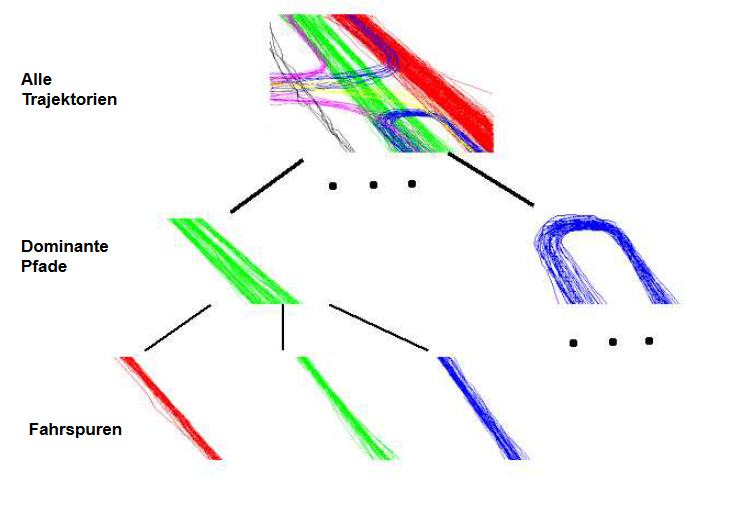
\includegraphics[width=0.5\linewidth]{../resources/img/RelatedWork/Fu_HierarchicalClustering}
    \caption[Zweistufiger Clustering-Vorgang von Hu et al.]{Zweistufiger Clustering-Vorgang von Hu et al. \cite[]{Hu2005}}
    \label{fig:relw_hu_two_step_cluster}
\end{figure}

Unter Verwendung des definierten Distanzmaßes werden die Trajektorien in einem zweistufigen Verfahren verarbeitet.
In den zwei Phasen werden, wie in Abbildung \ref{fig:relw_hu_two_step_cluster} dargestellt, zuerst dominante
Fahrpfade extrahiert, welche anschließend weiter in einzelne Fahrspuren untergliedert werden.
Als eigentliche Cluster-Algorithmen vergleichen die Autoren den \textit{Spectral-Clustering} Ansatz \cite[]{Ng2002}
mit einem \textit{Fuzzy-k-Means} Verfahren \cite[]{xie1991validity}.
Die Untersuchungen zeigen, dass der Spectral Clustering Ansatz nicht nur bessere Ergebnisse liefert, sonderen diese
über mehrere Durchläufe hinweg auch stabil sind, wohingegen die Resultate des Fuzzy-Ansatzes variieren.


% Junejo et al., 2004
\subsubsection*{Multi Feature Path Modeling for Video Surveillance}
Eine weitere Arbeit welche das Ziel hat, anormale Bewegungsmuster auf Basis von Trajektorien zu entdecken,
stammt von \cite[]{Junejo2004}. In diesem Fall geht es den Autoren allerdings nicht um das Finden von Fahrzeug-Fahrspuren,
sondern um die Extraktion von Laufpfaden von Fußgängern.
Die Bewegungsbahnen der Passanten werden aus Aufnahmen stationärer Überwachungskameras gewonnen und
als zwei-dimensionale Punktreihen repräsentiert.
Um die Trajektorien zu vergleichen, verwenden die Autoren die Hausdorff Distanz als Ähnlichkeitsmaß. 
Die üblicherweise negativen Eigenschaften dieses
Vergleichkriteriums (siehe Abschnitt \ref{sec:hausdorff_distance}), konkret die Missachtung der
Trajektorie-Orientierung, sind bei diesem Anwendungsfall kein Nachteil sondern gewünscht.
Da Fußgänger auf einem Pfad oder Weg in entgegengesetzte Richtungen gehen können, muss die Orientierung
ihrer Trajektorien ignoriert werden.
Auf Basis der Hausdorff Distanz erstellen Junejo et al. einen vollständigen Graphen, in welchem die Knoten Trajektorien
und die gewichteten Kanten den Distanzen zwischen Trajektorien entsprechen.
Sie zerlegen diesen Graphen mit Hilfe eines rekursiven \textit{min-cut}-Graphen-Algorithmus, welcher sich
an der Arbeit von \cite[]{boykov2004experimental} orientiert, und erhalten so die Cluster für die
extrahierten Fußgänger-Trajektorien.

% Atev et al., 2010
\subsubsection*{Clustering of Vehicle Trajectories}
In der Arbeit \cite[]{Atev2010} ist das Ziel der Autoren, ein Verfahren zu finden, mit welchem Fahrzeugtrajektorien
bestmöglich gruppiert werden können, ohne diese im Voraus anpassen zu müssen.
Sie vergleichen hierzu die Performance von drei unterschiedlicher Distanzmaße unter Verwendung von zwei Cluster-Algorithmen.
Primäres Augenmerk legen die Autoren auf ein von ihnen bereits in \cite[]{Atev2006} entwickeltes Distanzmaß, 
welches auf der Hausdorff Distanz basiert und sowohl die Orientierung von Trajektorien berücksichtigt
als auch robust gegenüber Ausreißern ist. Dieses neue Ähnlichkeitsmaß ist für zwei Trajektorien $P$ und $Q$
wie folgt definiert:

\begin{ceqn}
\begin{align}
    h_{\alpha, N, C}(P, Q) = \overset{\alpha}{\underset{p \in P}{ord}}\ \Big\{ \underset{q \in N_Q(C_{P,Q}(P))}{min} d(p, q) \Big\}
\end{align}
\end{ceqn}

Hierbei entspricht $C_{P,Q}$ einem Mapping $P \rightarrow Q$, welches einem Punkt $p \in P$ einen entsprechenden
Punkt $q \in Q$ zuweist, welcher die selbe relative Position in $Q$ besitzt wie $p$ in $P$.
$N_Q$ definiert ein Subset von $Q$ als Nachbarschaft des Punktes $q$. Zusammen definieren $N_Q$ und $C_{P,Q}$ eine
Struktur, in welcher der Abgleich der Trajektorien stattfindet. Dies ist visuell auch nochmals in Abbildung
\ref{fig:relw_atev_modh} dargestellt. Der Operator $ord_{p \in P}^{\alpha} f(p)$ selektiert jenen Wert aus $f(p)$, welcher
größer ist als $\alpha$-Prozent der Werte. 

\begin{figure}[H]
    \centering
    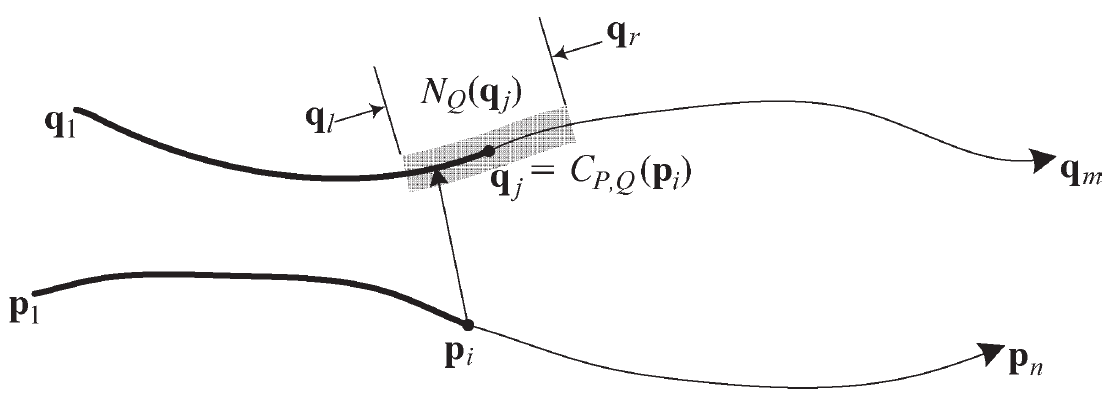
\includegraphics[width=0.6\linewidth]{../resources/img/RelatedWork/Atev_modHausdorff}
    \caption[Funktionsweise der modifizierten Hausdorff Distanz]{Funktionsweise der modifizierten Hausdorff Distanz \cite[]{Atev2010}}
    \label{fig:relw_atev_modh}
\end{figure}

Dank dieser Modifizierungen eignet sich das neue Ähnlichkeitsmaß gut für den Vergleich von Trajektorien:
$C_{P,Q}$ sorgt für den Einbezug der Orientierungen und über die Nachbarschaft $N_Q$ und $ord_{p \in P}^{\alpha} f(p)$
kann mit Ausreißern umgegangen werden.

Dieses Distanzmaß vergleichen Atev et al. unter Verwendung eines Spectral und eines Agglomerativen
Cluster-Algorithmus mit der \textit{Longest-Common Subsequence} (LCSS) und \textit{Dynamic Time Warping} (DTW) Distanz.
Die Ergebnisse der Untersuchungen für vier verschiedene Datensätze zeigen, dass die beste Cluster-Performance
mit Hilfe der modifizierten Hausdorff Distanz und des Spectral-Clustering erreicht wird.
Unter Verwendung der LCSS und DTW Distanzmaße, könnten die Autoren nicht die selben Resultate erzielen.

Dass das von Atev et al. vorgeschlagene Distanzmaß sehr gute Clusterergebnisse produziert, wurde auch von \cite{Morris2009}
bewiesen. In ihrer Untersuchung waren alledings die Ergebnisse, welche mithilfe des LCSS Maßes erreicht wurden,
ebenso gut, beziehungsweise teilweise sogar besser.

% Chen et al., 2011
\subsubsection*{Clustering of trajectories based on Hausdorff Distance}
Eine weitere interessante Arbeit zur Clusteranalyse von Trajektorien stammt von \cite[]{Chen2011}.
Die Autoren haben das Ziel, Muster in den Bewegungsbahnen von Hurrikans, welche im Zeitraum von 1850 bis 2010
über den Atlantik zogen, zu erkennen.
Sie verwenden hierzu einen angepassten DBSCAN Cluster-Algorithmus und das Hausdorff Distanzmaß.
Um die Missachtung der Orientierung kompensieren zu können, und zudem auch Ähnlichkeiten
in Sub-Trajektorien zu erkennen, wählen die Autoren eine etwas andere Darstellung der Trajektorien.
Sie definieren eine Bewegungsbahn als eine Folge sogenannter \textit{``Flow-Vektoren''}, welche neben
Positions- auch Richtungsinformationen enthalten. Ein solcher Vektor ist definiert über:

\begin{ceqn}
\begin{align}
    f_i = (x_i, y_i, dx_i, dy_i)
\end{align}
\end{ceqn}

wobei gilt:

\begin{ceqn}
\begin{align}
    dx_i = (x_{i+1} - x_i)/\sqrt{(x_{i+1} - x_i)^2 + (y_{i+1} - y_i)^2} \\
    dy_i = (y_{i+1} - y_i)/\sqrt{(x_{i+1} - x_i)^2 + (y_{i+1} - y_i)^2}
\end{align}
\end{ceqn}

Die Distanz zwischen zwei \textit{Flow-Vektoren} ist ihr euklidscher Abstand. Auf diese Weise wird bei
der Berechnung der Hausdorff Distanz (siehe Abschnitt \ref{sec:hausdorff_distance}) auch die Richtung
der Trajektorien berücksichtigt.
Um ähnliche Sub-Trajektorien entdecken zu können, teilen Chen et al. die Trajektorien an den Positionen
``charakteristischer'' Vektoren. Diese beschreiben Richtungsänderungen in einer
Bewegungsbahn und werden identifiziert über die Abweichungen in den Richtungskomponenten zweier
aufeinanderfolgender Flow-Vektoren. Dies ist anschaulich in Abbildung \ref{fig:relw_chen_flow_vector} dargestellt.

% TODO: Figure anpassen
\begin{figure}[H]
    \centering
    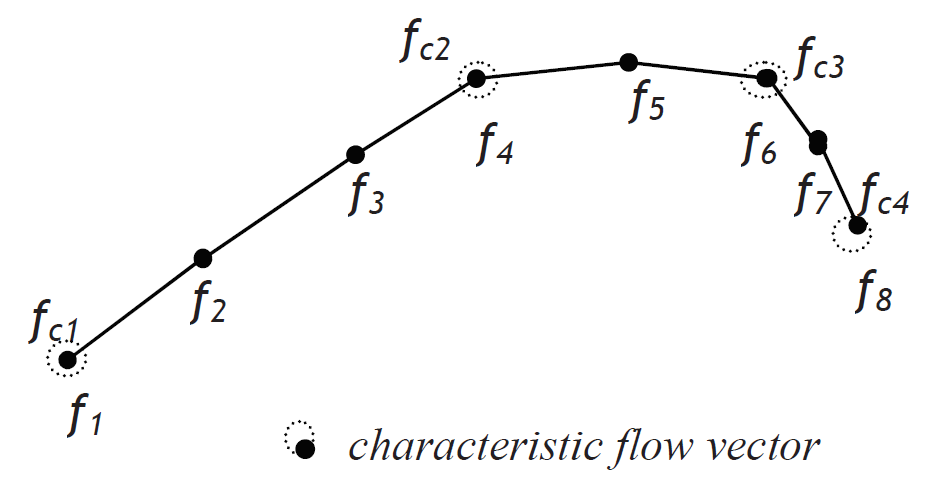
\includegraphics[width=0.45\linewidth]{../resources/img/RelatedWork/Chen_trajectory_splitting}
    \caption[Zerlegung einer Trajektorie in Sub-Trajektorien]{Zerlegung einer Trajektorie in Sub-Trajektorien \cite[]{Chen2011}}
    \label{fig:relw_chen_flow_vector}
\end{figure}

Die auf diese Weise erhaltenen Sub-Trajektorien werden von den Autoren mittels eines DBSCAN Algorithmus gebündelt.
Sie können so die üblichen Bewegungsbahnen von Hurrikans über dem Atlantik bestimmen.


% Vlachos et al., 2002
\subsubsection*{Discovering Similar Multidimensional Trajectories}
Die Arbeit \cite[]{Vlachos2002} thematisiert nicht direkt die Clusteranalyse von Trajektorien sondern
beschäftigt sich mit dem Vergleich von Bewegungsbahnen im drei-dimensionalen Raum. Konkret ist ihr Ziel,
Trajektorien vergleichen zu können, welche etwa die Handbewegungen beim Ausführen von Zeichensprache beschreiben.
Hierzu definieren die Autoren erstmals die Grundversion des LCSS Ähnlichkeitsmaßes, welches in vielen Arbeiten zum Einsatz
kommt \cite[]{Atev2006, Buzan2004, Chen2005}. Auf dessen Basis erstellen sie ein Distanzmaß, welche es ermöglicht
formgleiche aber im Raum verschobene Trajektorien zu finden.
Die Grundversion des LCSS Ähnlichkeitsmaßes und ein darauf basierendes einfaches Distanzmaß ist, nach Vlachos et al.,
bereits in Abschnitt \ref{sec:lcss_distance} definiert worden.
Dieses Maß erweitern die Autoren zudem wie folgt:

\begin{ceqn}
\begin{align}
    D2_{LCSS}(\delta, \epsilon, A, B) = 1 - \underset{f_{c,d} \in F}{max}\ D_{LCSS}(\delta, \epsilon, A, f_{c,d}(B))
\end{align}
\end{ceqn}

Hierbei ist $F$ eine Menge von Translations-Funktionen, welche die Trajektorien entlang der Achsen verschieben.
Sie besitzen die Form

\begin{ceqn}
\begin{align}
    f_{c, d}(A) = ((a_{x, 1} + c, a_{y, 1} + d), ..., (a_{x, n} + c, a_{y, n} + d))
\end{align}
\end{ceqn}

Abbildung \ref{fig:relw_vlachos_translation} veranschaulicht die Funktionsweise des Distanzmaßes. Es eignet sich immer dann, wenn Trajektorien
mit ähnlicher Form gefunden werden sollen, welche zudem eine gewisse räumliche Verschiebung aufweisen können.
Diese kann über die Größe von $F$ gesteuert werden.

\begin{figure}[H]
    \centering
    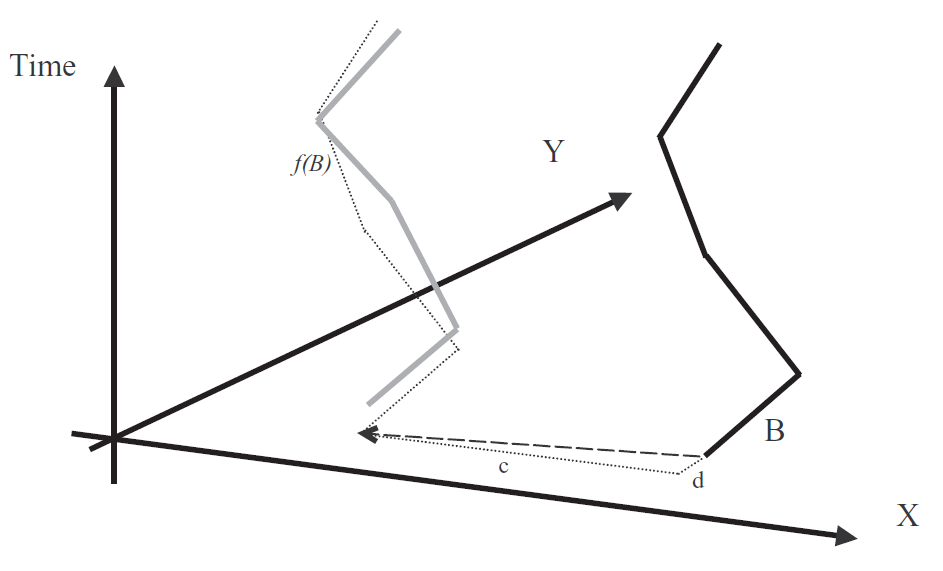
\includegraphics[width=0.55\linewidth]{../resources/img/RelatedWork/vlachos_translation}
    \caption[Verschiebung einer Trajektorie im Raum]{Verschiebung einer Trajektorie im Raum \cite[]{Vlachos2002}}
    \label{fig:relw_vlachos_translation}
\end{figure}

% Ren et al., 2014
\subsubsection*{Lane Detection in Video-Based Intelligent Transportation Monitoring via Fast Extracting and Clustering of Vehicle Motion Trajectories}

\cite[]{Ren2014} stellen in ihrer Arbeit ein interessantes Vorgehen zur Clusteranalyse von Trajektorien vor,
welches auf der \textit{Rough-Set}-Theorie beruht. Sie extrahieren Fahrzeugpositionen aus Aufnahmen stationärer
Überwachungskameras und stellen diese, wie die meisten Autoren, als Sequenzen zwei-dimensionaler
Punkte dar. Ihr Ziel ist anschließend, anhand einer Gruppierung der gewonnenen Fahrzeugtrajektorien,
die Spurmittelpunkte der Fahrbahnen zu bestimmen. Da ein nicht unerheblicher Anteil der Trajektorien Spurwechselvorgänge
enthält, welche eine Extraktion der Mittellinien erschweren, verwenden Ren et al. einen iterativen \textit{Rough-k-Means}
Algorithmus zur Clusterung der Trajektorien. Hierbei wird jedes Cluster über eine obere und untere Approximation beschrieben.
Die untere Approximation enthält dabei die Trajektorien, welche eindeutig der Spur zugeordnet werden können.
Die obere Näherung hingegen jene, welche Spurwechsel et cetera beschreiben. Bei der Berechnung der Spurmitten, werden
die Trajektorien der unteren Approximation höher gewichtet, als die der oberen. Ein sehr ähnlicher Cluster-Ansatz wurde
bereits in \cite[]{Lingras2004} vorgestellt.
Die initialen Mittellinien bestimmen die Autoren anhand einer \textit{Aktivitäts}- oder \textit{Heat}-Map,
welche sie während der Extraktion der Fahrzeugpositionen erstellen. Die Clusteranzahl $k$ muss händisch definiert werden.

Als Maß für die Distanz zwischen einer Trajektorie $A_x$ und einer Spurmitte $c_i$ verwenden Ren et al. die
Hausdorff Distanz $h(A_x, c_i)$. Für eine Trajektorie wird somit die nächste Mittellinie wie folgt gefunden:

\begin{ceqn}
\begin{align}
    h(A_x, c_m) = \underset{i = 1 ... k}{min}\ h(A_x, c_i)
\end{align}
\end{ceqn}

Hieraus ergibt sich die nachfolgende Definition für die Zuordnung der Bewegungsbahnen zu den Cluster-Näherungen:

\begin{ceqn}
\begin{align}
    \begin{cases}
        A_x \in \overline{C_m} \land A_x \in \overline{C_j} & \text{if } j \neq m \land \frac{h(A_x, c_j)}{h(A_x, c_m)} \leq \lambda \\
        A_x \in \underline{C_m} & \text{otherwise}
    \end{cases}
\end{align}
\end{ceqn}

Es gilt $1 \leq \lambda \leq 1.5$. $\overline{C_m}$ und $\underline{C_m}$ entsprechen der oberen und unteren
Näherung des $m$-ten Clusters und $\underline{C_m} \subseteq \overline{C_m}$.
Nachdem in jeder Iteration des Cluster-Vorgangs die Näherungen auf diese Weise bestimmt wurden, werden die neue Mittellinien
anhand Gleichung \ref{eq_ren_rough} errechnet.

\begin{ceqn}
\begin{align}
    \label{eq_ren_rough}
    c_i =
    \begin{cases}
        \frac{w_l \sum_{A_x \in \underline{C_i}} A_x}{|\underline{C_i}|} + \frac{(1 - w_l) \sum_{A_x \in (\overline{C_i} - \underline{C_i})} A_x}{|\overline{C_i} - \underline{C_i}|} & \text{if } \overline{C_i} \neq \underline{C_i} \\
        \frac{\sum_{A_x \in \underline{C_i}} A_x}{|\underline{C_i|}} & \text{otherwise}
    \end{cases}
\end{align}
\end{ceqn}

Als Gewichtungen $w_l$ verwenden Ren et al. Werte im Bereich $[0.5, 1]$. $| \cdot |$ entspricht hier der Kardinalität einer Menge.

Unter Verwendung dieser Clustering-Methode ist es den Autoren von \cite[]{Ren2014} möglich, auch bei einer hohen Anzahl von
Ausreißern und Spurwechselvorgängen, stabile Spurmittellinien zu bestimmen. Ergebnisse, welche dies zeigen, sind in Abbildung
\ref{fig:relw_ren_example_detection} dargestellt.

\begin{figure}[H]
    \centering
    \includegraphics[width=0.9\linewidth]{../resources/img/RelatedWork/ren_examples_detection}
    \caption[Ergebnisse der Spurmittellinien-Erkennung (Ren et al.)]{Ergebnisse der Spurmittellinien-Erkennung \cite[]{Ren2014}}
    \label{fig:relw_ren_example_detection}
\end{figure}


\section{Erkennung von Fahrspuren}
\label{sec:rw_lane_detection}
% Hier Arbeiten vorstellen, welche (prim. auf Basis von Traj.Clustern) versuchen Fahrspuren / Fahrbahnen
% zu erkennen
% Auch übliche Ansätze vorstellen, welche nicht mit Traj. arbeiten (erwähnen häufig optisch / aus Fahrzeugen)

Primäres Ziel dieser Arbeit ist es, Fahrspuren zuverlässig in Videoaufnahmen erkennen zu können. Dieser Abschnitt
geht daher auf einige Arbeiten ein, welche ähnliches ebenfalls versuchen.

Die Mehrzahl der Veröffentlichungen in diesem Bereich, löst das Problem, indem sie nach visuellen Merkmalen,
primär Spurtrennlinien, in Videoaufnahmen suchen. Die Aufnahmen werden dabei entweder von stationären Kameras,
von bemannten oder unbemannten Luftfahrzeugen oder einem Fahrzeug selbst gemacht. Zur Extraktion der Merkmale werden
üblicherweise Methoden aus den Gebieten des maschinellen Sehen (CV) oder maschinellen Lernens (ML) verwendet. % TODO: Abkzg.
Arbeiten, welche CV-basierte Ansätze verfolgen, stammen beispielsweise von \cite[]{Lai2000}, \cite[]{McCall2006} oder \cite[]{Aly2008}.
ML-gestützte Arbeiten wurden dahingegend unter anderem von \cite[]{Kim2008} und \cite[]{Gopalan2012} veröffentlicht.
% Ein mögliches Anwendungsgebiet für solche Ansätze ist Beispiel die Entwicklung eines Spurhalte-Assistenten.

Da oben genannte Ansätze, wie bereits zu Beginn der Arbeit erläutert, aufgrund von Verdeckungen oder Änderungen
in der Belichtung problematisch sind, werden nachfolgend ausschließlich Arbeiten vorgestellt, welche Fahrspuren
aus Trajektoriedaten extrahieren. Hierbei setzten sie als ersten Schritt alle auf eine Clusteranalyse von Trajektorien.
In der Repräsentation und Extraktion der Fahrspuren variieren die Ansätze hingegen.


% Fu et al. & Junejo et al.
%   Clustering und dann Bestimmung Envelopes basierend auf Varianz der Trajektorien in Cluster
\subsubsection*{Similarity based vehicle trajectory clustering and anomaly detection}
% Envelope (Covarianz) aus Clustern


% Makris et al., 2005
\subsubsection*{Learning Semantic Scene Models From Observing Activity in Visual Surveillance}
% Erstellen Hüllen für Traj. --> Traj zu Bahn zuordnen


% Morris et al., 2011
\subsubsection*{Trajectory Learning for Activity Understanding: Unsupervised, Multilevel, and Long-Term Adaptive Approach}
% HMM


% Hsieh et al., 2006
% Automatic Traffic Surveillance System for Vehicle Tracking and Classification
\subsubsection*{Automatic Traffic Surveillance System for Vehicle Tracking and Classification}
% Heat Map --> Spurmittellinien --> Begrenzer aus Mittellinien bestimmen


\section{Defizite vorhandener Lösungen und benötigte Neuerungen}
\label{sec:rw_deficites}

% Eigentlich nichts zur Spurerkennung auf bspw. Kreuzungen etc.
%   Wenn Spur dann immer nur Spur für gesamtes Cluster (kein Partitioning)

% Meiste Aufnahmen sind Frontal-Aufnahmen auf Straße --> keine Verzerrungen
%!TEX root = ../Thesis.tex

\chapter{Untersuchung möglicher Straßentopologien}
\label{cha:street_topologies}

% Beschreibung möglicher (Auswahl) Straßentopologien und ihrer Herausforderungen für die Erkennung von Fahrbahnen
% Idealerweise immer Bild einer entsprechenden Topologie und der entsprechenden Roh-Trajektorien

% Erläuterung: Was ist eine "Fahrspur" in dieser Arbeit. (d.h. nicht notwendigerweise eine Spur, wie sie auf Straße markiert ist. Beschreibt übliche Fahrbahn eines Fahrzeugs?!)

% Landstraßen (ein / zweispurig),
\section{Landstraßen}

% einfachste Straßentopologie, daher einfach darin Fahrspuren zu identifizieren
% entweder klar separierte Fahrspuren, welche parallel zueinander laufen oder eine (breite) Spur, welche in beide Richtungen genutzt wird
% üblicherweise wenig Abzweigungen, Einfahren etc.

% Bild einer leicht gekrümmten / gewundenen Landstraße


% Autobahnen (inkl. Auffahrten, Abfahrten)
\section{Autobahnen}

% ähneln Landstraße, Spuren hier immer separiert. Fahrzeuge fahren in auf einer Spur in eine Richtung
% Bahnen üblicherweise breiter.
% Auffahrten und Abfahren existieren

% Bild Entennest


% Kreuzungen (inkl. Abbiegespuren)
\section{Kreuzungen}

% Fahrbahnen kreuzen sich, geregelt über Ampelanlagen oder Rechts-vor-Links
% Abbiegespuren
% Fahrspuren überlagern sich. Sinnvolle Aufteilung

% Kreisverkehre
\section{Kreisverkehre}

% 12 Bewegungsbahnen durch Kreisverkehr (ausgenommen 360Grad Wendungen etc.)
% schwierig zu definieren, wie fahrspuren durch Kreisverkehr verlaufen
% Welche partitionieren
% Werden alle Bahnen richtig erkannt? Viele Überdeckungen. Richtig geclusterd?
%!TEX root = ../Thesis.tex

\chapter{Konzeption des Spurerkennungs-Moduls}
\label{cha:konzeption}

In diesem Kapitel wird das zu entwickelnde Teilmodul \textit{``Spurerkennung''}
der Anwendung \textit{Vehicle-Tracker} konzipiert. Hierzu wird zuerst dessen Rolle und Position im Gesamtkontext
der Anwendung betrachtet. Anschließend werden die Anforderungen und ein grober Entwurf des Moduls vorgestellt.

\section{Überblick über das Gesamtsystem}

Das Modul \textit{Spurerkennung} dient der Erreichung der in Abschnitt
\ref{sec:motivation_goals} definierten Ziele. Erstellt wird es im Rahmen des MEC-View Teilprojektes
\textit{Luftbeobachtung} als Teilmodul der Anwendung \textit{Vehicle-Tracker}.
Abbildung \ref{fig:concept_laneDetection_context} gibt einen Überblick über das System.
Es werden hierbei jene Module beziehungsweise Schritte vorgestellt, welche mit der Spurerkennung in
Zusammenhang stehen.

\begin{figure}[H]
    \centering
    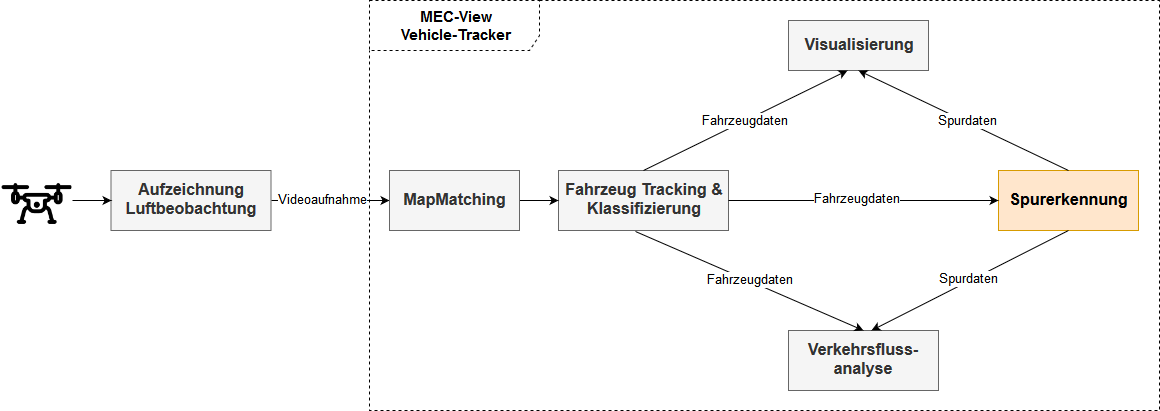
\includegraphics[width=\linewidth]{resources/img/konzeption/Context_LaneDetection}
    \caption{Kontext des Moduls Spurerkennung}
    \label{fig:concept_laneDetection_context}
\end{figure}

Die mithilfe von Drohnen erstellten Videoaufnahmen können in der MEC-View \textit{Vehicle-Tracker} Applikation
verarbeitet und analysiert werden. In einem ersten Schritt namens \textit{``MapMatching''} wird für eine Aufnahme
ein Weltkoordinatensystem in Metern definiert. Anschließend werden die Positionen
der Fahrzeuge bestimmt. Diese ersten zwei Schritte sind in Kapitel \ref{sec:position_extraction} genauer beschrieben.
Die Fahrzeuginformationen, insbesondere die Positionsinformationen, dienen dem \textit{Spurerkennung}-Modul
als Eingabe. Aus ihnen extrahierte Spurdaten können anschließend in der Anwendung visualisiert werden oder in Kombination
mit den Fahrzeuginformationen zur Analyse des Verkehrsflusses eingesetzt werden.


\section{Anforderungen an das Modul}
\label{sec:requirements}

In diesem Abschnitt werden die wichtigsten funktionalen und nicht funktionalen Anforderungen
an das Modul Spurerkennung festgehalten.

\subsection{Funktionale Anforderungen}

\paragraph{Anforderung 1000 (Top-Level)}
Das \textit{Spurerkennungs}-Modul soll es ermöglichen, mithilfe der Anwendung \textit{Vehicle-Tracker},
automatisch Fahrspuren in Luftaufnahmen anhand von Trajektoriedaten zu erkennen.

\paragraph{Anforderung 2000}
Das Modul soll die Erkennung von Fahrspuren in den folgenden Straßentopologien unterstützen:

\begin{itemize}
    \item Gerade Fahrbahnen
    \item Kreuzungen
    \item Kreisverkehre
    \item Sich öffnende oder schließende Spuren (z.B. Be- oder Entschleunigungsstreifen)
\end{itemize}

\paragraph{Anforderung 2100}
Das Modul soll unabhängig vom Aufnahmewinkel der Kamera Fahrspuren zuverlässig aus Videoaufnahmen ableiten können.

\paragraph{Anforderung 2200}
Das Modul soll Fahrspuren bei Überlagerungen sinnvoll partitionieren können.

\paragraph{Anforderung 2300}
Das Modul soll die Plausibilität von Fahrspuren bewerten können und nicht plausible Spuren entfernen.

\paragraph{Anforderung 2400}
Das Modul soll die Enden benachbarter und paralleler Fahrspuren aneinander angleichen.

\paragraph{Anforderung 2500}
Das Modul soll es ermöglichen, die aus den Trajektorien abgeleiteten Fahrspuren in der Anwendung \textit{Vehicle-Tracker}
zu visualisieren.

\subsection{Nicht funktionale Anforderungen}

\paragraph{Anforderung 3000}
Das \textit{Spurerkennungs}-Modul muss robust mit Ausreißern und Tracking-Fehlern in den Trajektorien umgehen können.

\paragraph{Anforderung 3100}
Die Performance des Spurerkennung-Vorgangs ist nicht von höchster Priorität. Eine Erkennung soll allerdings
dennoch maximal wenige Minuten dauern.


\section{Entwurf des Moduls}
\label{sec:design}

In diesem Abschnitt wird, basierend auf den Erkenntnissen der Literaturrecherche und den Anforderungen,
ein grober Entwurf des \textit{Spurerkennung}-Moduls vorgestellt.

Das Modul enthält einen Algorithmus, welcher aus Fahrzeugtrajektorien Fahrspuren ableitet.
Die Grundfunktionsweise dieses Algorithmus ist in Abbildung \ref{fig:concept_laneDetection_activity}
in Form eines Aktivitätsdiagrams dargestellt.

\begin{figure}[H]
    \centering
    \includegraphics[width=0.8\linewidth]{resources/img/konzeption/activity_laneDetection}
    \caption{Basis-Ablauf des Spurerkennungs-Algorithmus}
    \label{fig:concept_laneDetection_activity}
\end{figure}

Die einzelnen Schritte des Algorithmus werden im \textit{Spurerkennungs}-Modul als einzelne Komponenten
implementiert.
Die \textit{Vehicle-Tracker} Applikation ist in Java und Scala implementiert. Ihre Benutzeroberfläche basiert
auf JavaFX. Das in dieser Arbeit erstellte Modul wird komplett mit Scala umgesetzt.

% Die nachfolgenden Kapitel beschreiben, wie die einzelnen Schritte des Algorithmus aus
% Abbildung \ref{fig:concept_laneDetection_activity} realisiert werden und welche Probleme hierbei
% überwunden werden müssen.
%!TEX root = ../Thesis.tex

% Umsetzung

\chapter{Clustering von Fahrzeugtrajektorien}
\label{cha:realisation_clustering}

% Feature Selection (Positionen Relevant)
% Beispiel für Rohdaten (Kreuzung)

\section{Vorverarbeitung der Roh-Trajektorien}
\label{sec:realisation_preprocessing}

% Resampling
% Aussortierung zu kurzer Trajektorien
% Aussortierung stehender Trajektorien
% Trimmen Truck-Trajektories

\section{Gruppierung der Trajektorien}
\label{sec:realisation_clustering}

% genaue Beschreibung des Vorgehens, bis finale Clustering Lösung erreicht wurde
% Ansätze: Gründe, Stärken, tatsächliche Problem
% Ansatz A:
%   Mod. Hausdorff Distanz und Spectral Clustering (bas. auf Avet et al.)
%   Weil: SC performant, deterministisch, oft verwendet
%   Probleme: Clusteranzahl Bestimmung, Umgehen mit Ausreißern, Tatsächliche Ergebnisse nicht gut
% Ansatz B:
%   LCSS Distanz (in anderen Papern gute Ergebnisse) (impl. mittels bottom up dyna. programmierung, Verwendung Eucl. Dist.)
%   Wieso D2 aus Vlachos et al. verwendet? (Verschiebung unerwünscht)
%   DBSCAN Clustering
%   --> DM kann besser mit Ausreißern umgehen und DBSCAN berücksichtigt diese auch
%   bessere Ergebnisse


\chapter{Fahrbahn-Bestimmung aus Trajektorie-Clustern}
\label{cha:lane_definition}

% Cluster-Bereinigung: Entfernen von Outliern (Spurwechselvorgänge)
% Bestimmung Referenz-Trajektorie
% Bestimmung von Spur-Envelopes
% Partitionierung der initialen Spur-Schätzungen

\chapter{Fahrbahn Klassifizierung}
\label{cha:realisation_lane_classification}
%!TEX root = ../Thesis.tex

% \chapter{Realisierung LaneDetection in MEC-View TrackerApplication Software}
% \label{cha:realisation_tracker}
%!TEX root = ../Thesis.tex

\chapter{Auswertung und Ergebnisse}
\label{cha:results}

Die Stärken, Schwächen und Ergebnisse des entwickelten Algorithmus werden im nachfolgenden Kapitel
zusammengefasst, diskutiert und ausgewertet. Es wird zuerst abschnittsweise auf die drei primären Schritte
des entwickelten Spurerkennungsverfahrens eingegangen. Endergebnisse werden anschließend
in Form von Screenshots vorgestellt, in welchen die erkannten Fahrspuren zu sehen sind.

\section{Evaluierung der Datenvorverarbeitung}
\label{sec:results_eval_dataprocessing}

Die Datenvorverarbeitung ist ein wichtiger Teilschritt bei der Erkennung von Fahrspuren. Nur wenn aus
den Roh-Trajektorien die meisten Defekte entfernt wurden, können die nachfolgenden
Schritte zuverlässig funktionieren. Die angewandten Schritte zur
Entfernung der Defekte sind in Abschnitt \ref{sec:realisation_preprocessing} beschrieben.

Anhand von Abbildung \ref{fig:real_result_2nd_Prepro} im Umsetzungskapitel wurde bereits gezeigt,
dass die Datenvorverarbeitung grundsätzlich funktioniert.
In Abbildung \ref{fig:results_prePro_heilbronner} sind nun die Roh-Trajektorien und bereinigten Bewegungsbahnen
eines weiteren Datensatzes dargestellt, welcher von der Heilbronner-Straße in Stuttgart stammt.

\begin{figure}[H]
    \centering
    \subfloat[]{{
        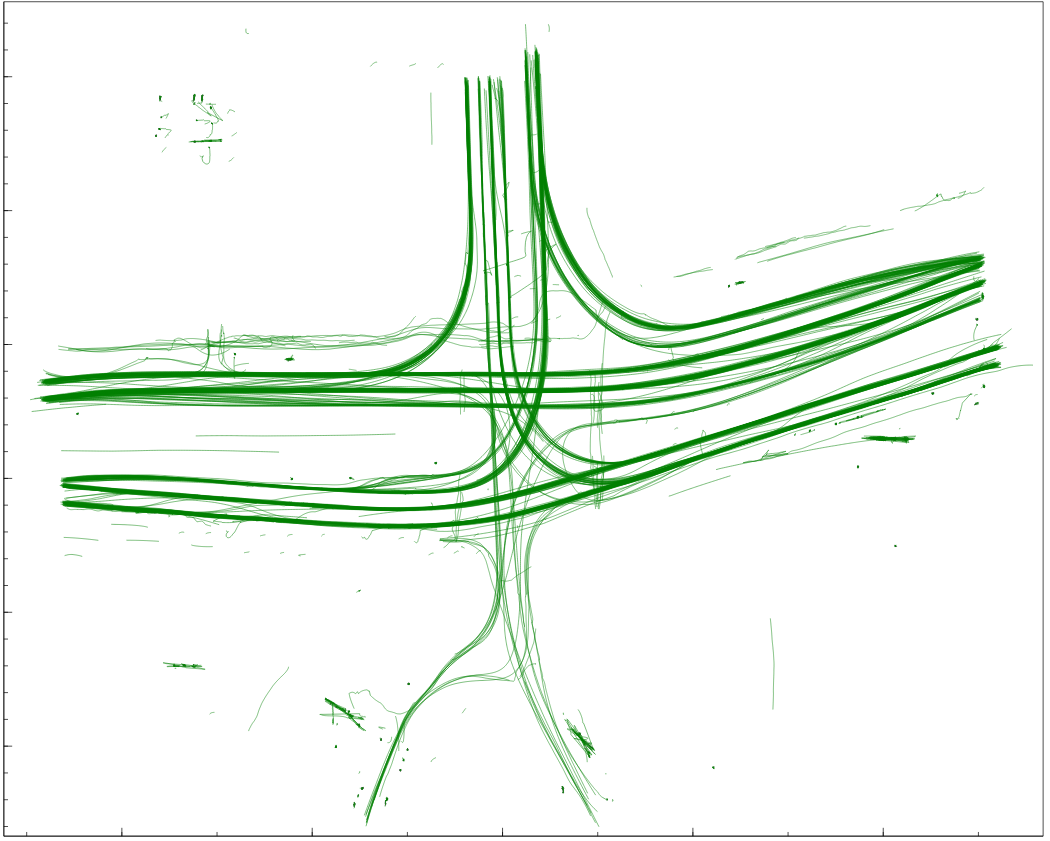
\includegraphics[align=c, width=0.33\linewidth]{resources/img/results/Heilbronner/rawTrajectories}
    }}
    \qquad \qquad
    \subfloat[]{{
        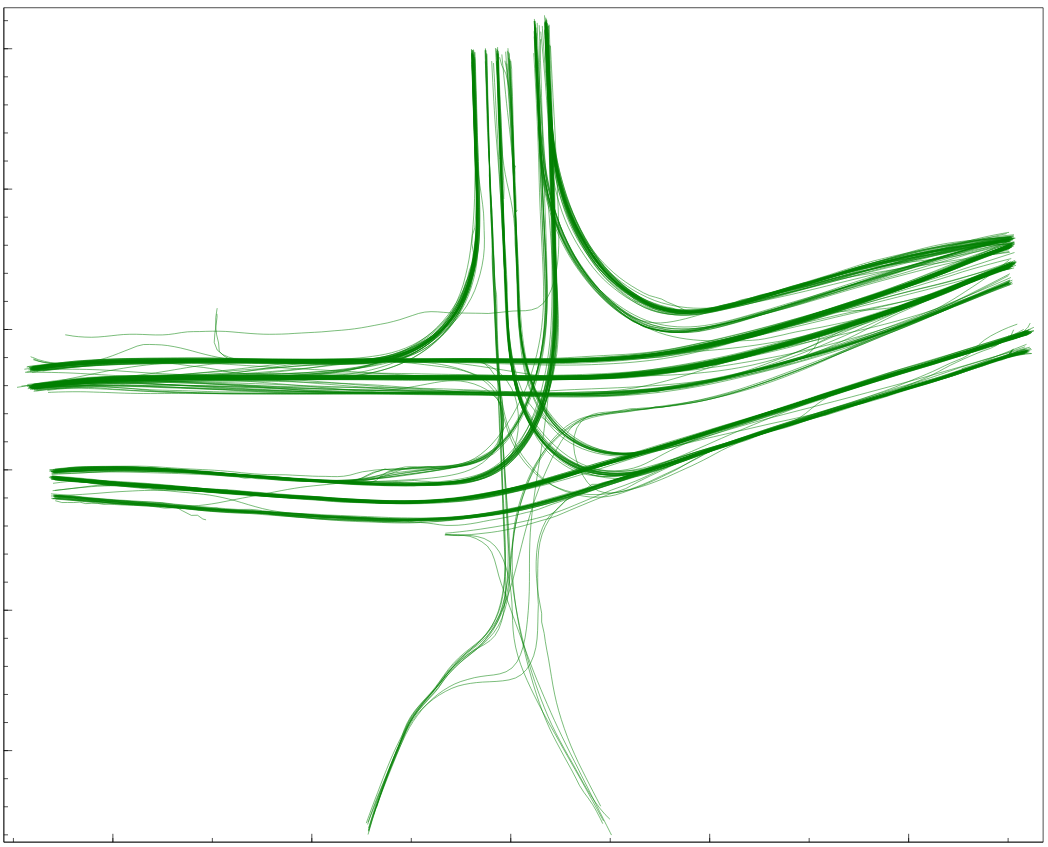
\includegraphics[align=c, width=0.33\linewidth]{resources/img/results/Heilbronner/preProTrajs}
    }}
    \caption[Ergebnis Trajektorie-Vorverarbeitung der Heilbronner-Straße]
            {Fahrzeugtrajektorien im Rohformat a), vorverarbeitete Trajektorien b) - Datensatz \textit{Heilbronner-Straße}}
    \label{fig:results_prePro_heilbronner}
\end{figure}

Die Plots zeigen gut, dass die vielen in a) vorkommenden Defekte entfernt wurden. Von den
circa 1050 Roh-Trajektorien im ursprünglichen Datensatz bleiben nach der Vorverarbeitung etwa 450 intakte
Bewegungsbahnen übrig. Die Mehrzahl der Defekte in diesem Fall stammt von \textit{False-Positive}-Detektionen
und unterbrochener Fahrzeug-Detektionen (siehe Abschnitt \ref{sec:grund_challenges_reconstruction}).

Ein problematisches Verhalten der Datenvorverarbeitung wurde beim Testen der Spurerkennung anhand eines
Datensatzes aus Steinheim deutlich. In Abbildung \ref{fig:results_horizon_problem} a) ist der
untersuchte Straßenabschnitt dargestellt.

\begin{figure}[H]
    \centering
    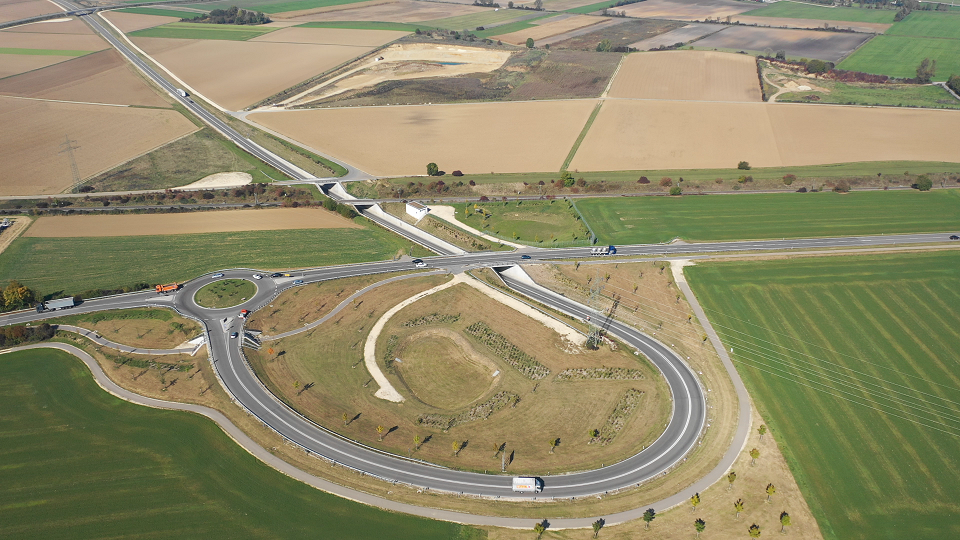
\includegraphics[width=0.5\linewidth]{resources/img/results/Steinheim/steinheim}
    \caption[Straßenabschnitt Datensatz Steinheim]
            {Straßenabschnitt Datensatz Steinheim mit am Horizont verschwindenden Fahrspuren}
    \label{fig:results_horizon_problem}
\end{figure}

Schwierig an dieser Aufnahme ist, dass die Fahrzeuge, welche sich auf der oben links startenden Fahrbahn bewegen,
am Anfang beziehungsweise Ende ihrer Fahrt sehr klein sind. Da Fahrzeuge in einer Videoaufnahme ab einer gewissen Größe
nurnoch sehr unzuverlässig detektiert werden, brechen die Trajektorien in diesem Fall auf sehr
unterschiedlichen Höhen ab.
Aufgrund der stark variierenden Start- und End-Positionen, entfernt der in Abschnitt
\ref{sec:real1_remove_broken_trajectories} beschriebene Algorithmus zur Identifikation unterbrochener
Trajektorien, auch die meisten Bewegungsbahnen von Fahrzeugen, welche sich auf den Horizont zu oder von im weg bewegen.
Somit können für diese Fahrspuren auch keine Spur-Geometrien bestimmt werden.
Dieses Verhalten kann immer dann auftreten, wenn Fahrbahnen auf einen von der Kamera weit entfernten Horizont zulaufen.

Da Fahrzeuge im Bereich eines solchen Horizonts grundsätzlich unzuverlässig erkannt werden, ist auch eine Fahrverhaltensanalyse
mithilfe von Fahrspuren hier nicht sinnvoll. Es wurde daher entschieden, dem Anwender die Möglichkeit zu geben, eine
Horizont-Linie zu definieren. Diese sollte vor der Höhe liegen, ab welcher die Fahrzeugerkennung unzuverlässig wird.
In einem ersten Vorverarbeitungsschritt werden alle Trajektorie-Punkte oberhalb dieser
Linie entfernt. Dank der Beschneidung der Trajektorien bleiben diese in den nachfolgenden Verarbeitungsschritten
erhalten und es können Spuren im gewünschten Ausschnitt erkannt werden.

Mit Ausnahme des unerwünschten Verhaltens im Fall von Trajektorien, welche am Horizont sehr unterschiedliche Start-
beziehungsweise End-Positionen besitzen, funktioniert die Datenvorverarbeitung zuverlässig und wie gewünscht.
Voraussetzung dafür, dass nach der Vorverarbeitung noch genug Trajektorien vorliegen, welche weiterverarbeitet werden können,
ist, dass in den Rohdaten ausreichend intakte Bewegungsbahnen vorhanden sind.

\section{Evaluierung der Clusteranalyse}
\label{sec:results_eval_clustering}

Die Clusteranalyse der Trajektorien bildet die Grundlage für die anschließende Bestimmung der Spur-Geometrien.
Sie ist daher ein kritischer Bestandteil der Spurerkennung. Der in dieser Arbeit eingesetzte Ansatz zur
Gruppierung der Trajektorien wurde in Abschnitt \ref{sec:real_ansatz_dbscan_lcss} beschrieben.
Hier wurden auch bereits Ergebnisse der Clusteranalyse für die Datensätze \textit{Esslingen} und
\textit{Neckartor} vorgestellt.

Da der angewandte Clustering-Algorithmus die vollständigen Verläufe der
Trajektorien vergleicht, ist die wichtigste Vorraussetzung zur Identifikation eines Clusters, dass ausreichend
Trajektorien vorliegen, welche eine identische Bewegung durch einen Straßenabschnitt beschreiben.
In Abschnitt \ref{sec:results_clustering_dbscan_lcss} wurde erwähnt, dass ein Cluster mindestens aus
fünf Trajektorien bestehen muss. Diese Untergrenze wurde gewählt, um nicht zu viele Cluster zu identifizieren, welche
eigentlich keine Fahrspur beschreiben. Würde die Grenze niedriger angesetzt werden, so würden beispielsweise
vermehrt Cluster aus Trajektorien gebildet, welche Überholvorgänge beschreiben.

In den meisten Datensätzen, anhand derer der in dieser Arbeit entwickelte Algorithmus getestet wurde,
existierten ausreichend Trajektorien pro Fahrspur, um diese zuverlässig zu identifizieren. Eine Ausnahme
stellt der Datensatz von der Heilbronner-Straße in Stuttgart dar, dessen Trajektorien bereits
in Abschnitt \ref{sec:results_eval_dataprocessing} dargestellt sind. In Teil b) dieser Abbildung
wird deutlich, dass die Fahrspuren im unteren Bereich des Straßenabschnitts nur wenig befahren sind.
Dies wirkt sich auch auf das Ergebnis der Clusteranalyse aus, welches in Abbildung \ref{fig:results_clusters_heilbronner} dargestellt ist.
Zwar existieren ausreichend Trajektorien, welche sich von oben nach unten links bewegen, allerdings können
keine Gruppen aus den Trajektorien gebildet werden, welche sich unten rechts befinden.
Die wenigen in diesem Bereich existierenden Trajektorien haben sehr unterschiedliche Bewegungsbahnen,
weshalb hier kein Cluster identifiziert wird.

\begin{figure}[H]
    \centering
    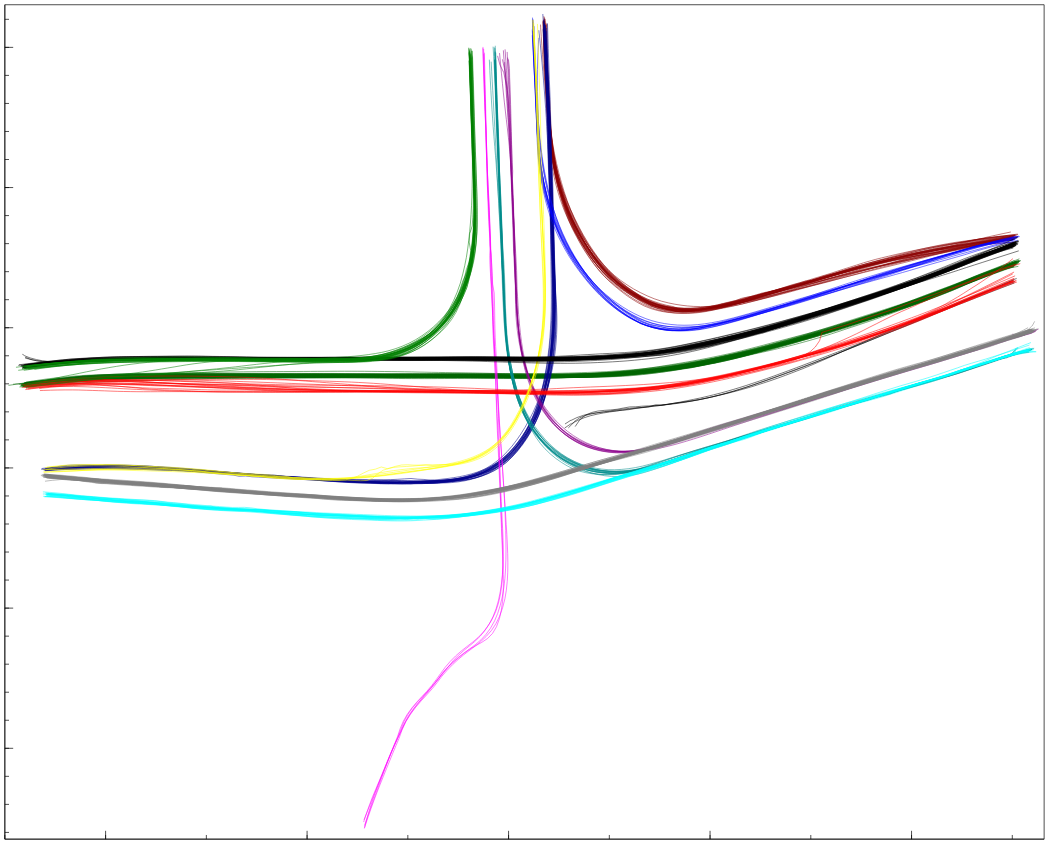
\includegraphics[width=0.35\linewidth]{resources/img/results/Heilbronner/filteredClusters_Heilbronner}
    \caption{Ergebnis Trajektorie-Cluster der Heilbronner-Straße}
    \label{fig:results_clusters_heilbronner}
\end{figure}

Die Plots in Abbildung \ref{fig:results_clusters_neckartor} a) und b) zeigen das Ergebnis der Clusteranalyse für
den \textit{Neckartor}-Datensatz, aus welchem vor Anwendung des Algorithmus zufällig 50\% der Trajektorien entfernt wurden.

\begin{figure}
    \centering
    \subfloat[]{{
        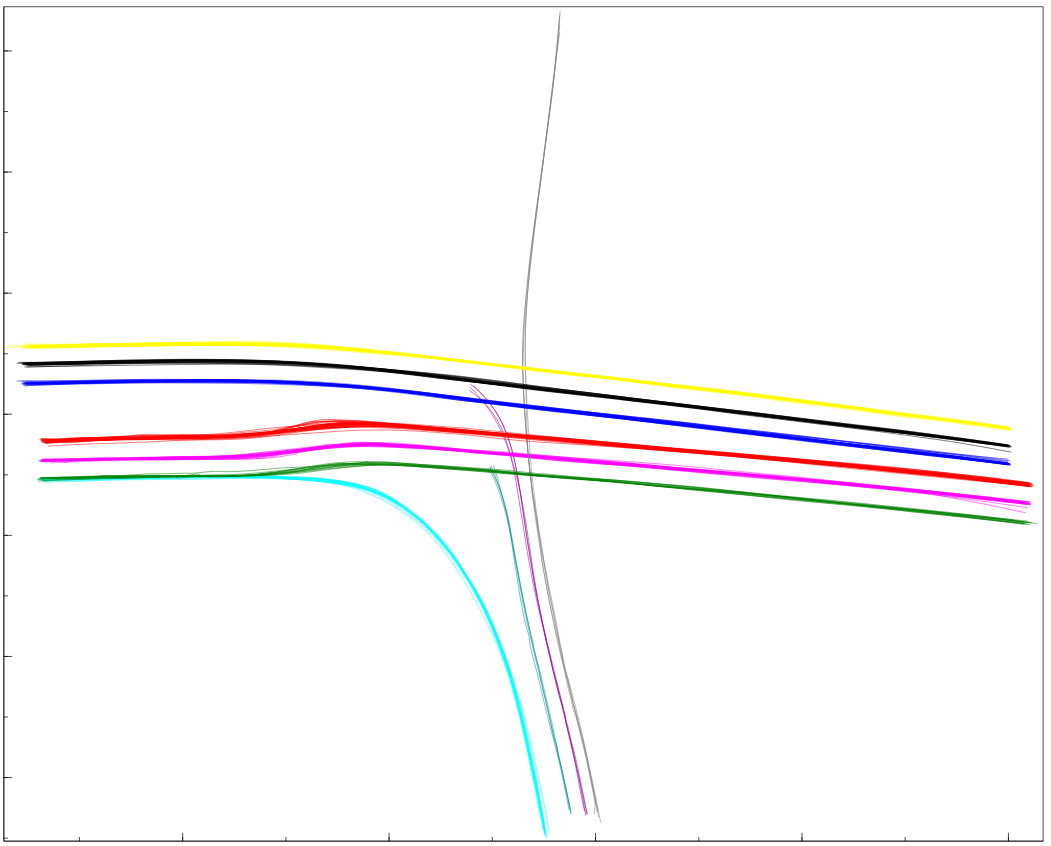
\includegraphics[align=c, width=0.31\linewidth]{resources/img/results/Neckartor/filteredClusters1}
    }}
    \qquad \qquad
    \subfloat[]{{
        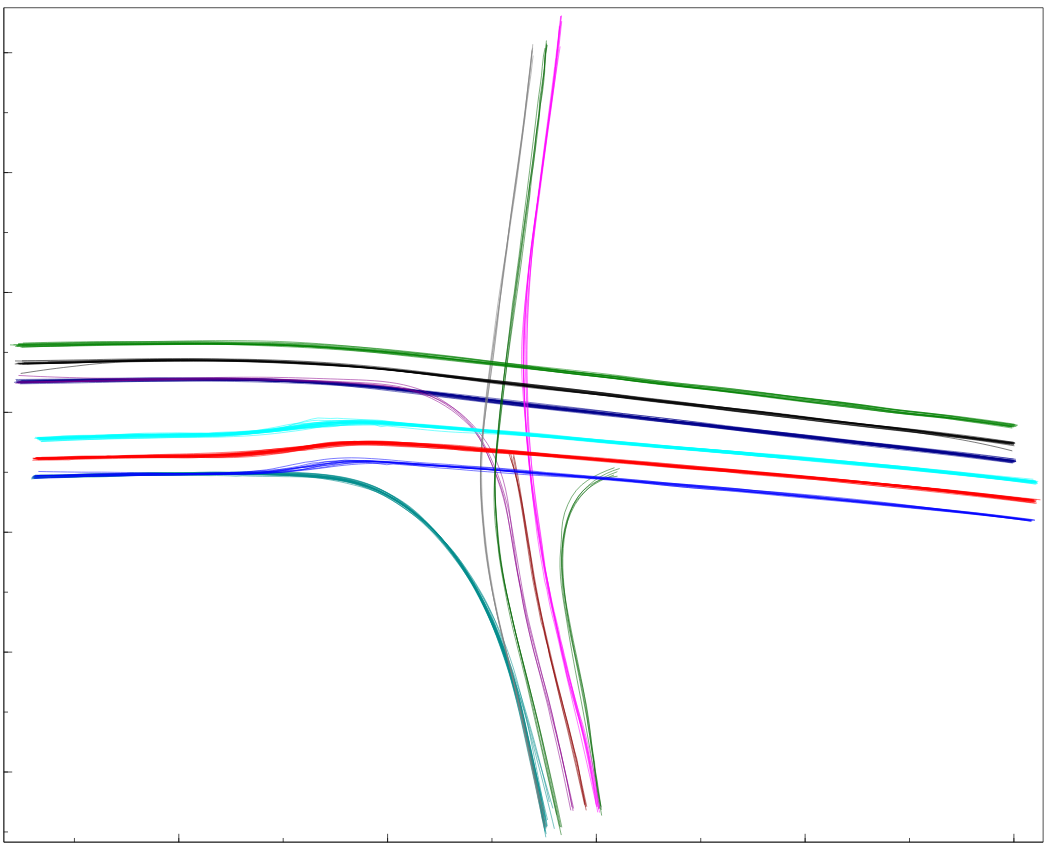
\includegraphics[align=c, width=0.31\linewidth]{resources/img/results/Neckartor/filteredClusters2}
    }}
    \caption[Ergebnisse Test Clusteranalyse auf Neckartor Datensatz]
            {Trajektorie-Cluster des Neckartor-Datensatzes nach zufälliger Entfernung von 50\% der Trajektorien}
    \label{fig:results_clusters_neckartor}
\end{figure}

Auch hier wird deutlich, dass das Ergebnis maßgeblich von der Anzahl der Trajektorien pro Spur abhängt.
In Plot a) wurden vorwiegend vertikal verlaufende Trajektorien entfernt, weshalb hier nur wenige Spurcluster identifiziert werden.
In Plot b) wurden hingegen, trotz des Fehlens von 50\% der Trajektorien, fast alle Spurcluster erkannt
(vergleiche Abbildung \ref{fig:real_turning_lane} c)).

Außer von der Anzahl der Trajektorien, hängt das Ergebnis der Clusteranalyse primär von den gewählten
Parametern des DBSCAN Clusteralgorithmus ab. Die Standardparameter für das Clustering-Verfahren wurden
in Abschnitt \ref{sec:results_clustering_dbscan_lcss} definiert. In Abschnitt \ref{sec:real1_adjustment_clustering_parameter}
wurde zudem ein Verfahren vorgestellt, mit dessen Hilfe der Parameter $\epsilon_{DBSCAN}$
automatisch angepasst wird, wenn die Qualität der ermittelten Spur-Cluster nicht den Erwartungen entspricht.
Alle bislang in der Arbeit gezeigten Ergebnisse der Clusteranalysen wurden ohne manuelle Parameteranpassungen bestimmt.
Die Spur-Cluster beschreiben die in einem Straßenabschnitt existierenden Fahrspuren meist sehr gut,
weshalb auch die daraus abgeleiteten Spur-Geometrien die Fahrbahnen gut abbilden.

In speziellen Fällen kann es allerdings vorkommen, dass trotz schlechter Clustering-Ergebnisse
keine automatische Neuparametrisierung und Durchführung der Clusteranalyse vorgenommen wird.
In dieser Situation können nur über eine manuelle Parametrisierung die Spur-Cluster zuverlässig identifiziert werden.
Dies trifft beispielsweise auf den Datensatz \textit{Steinheim} zu. Die unter Einsatz der Standardparameter
ermittelten Spur-Cluster sind in Abbildung \ref{fig:results_clusters_steinheim} a) dargestellt.

\begin{figure}
    \centering
    \subfloat[]{{
        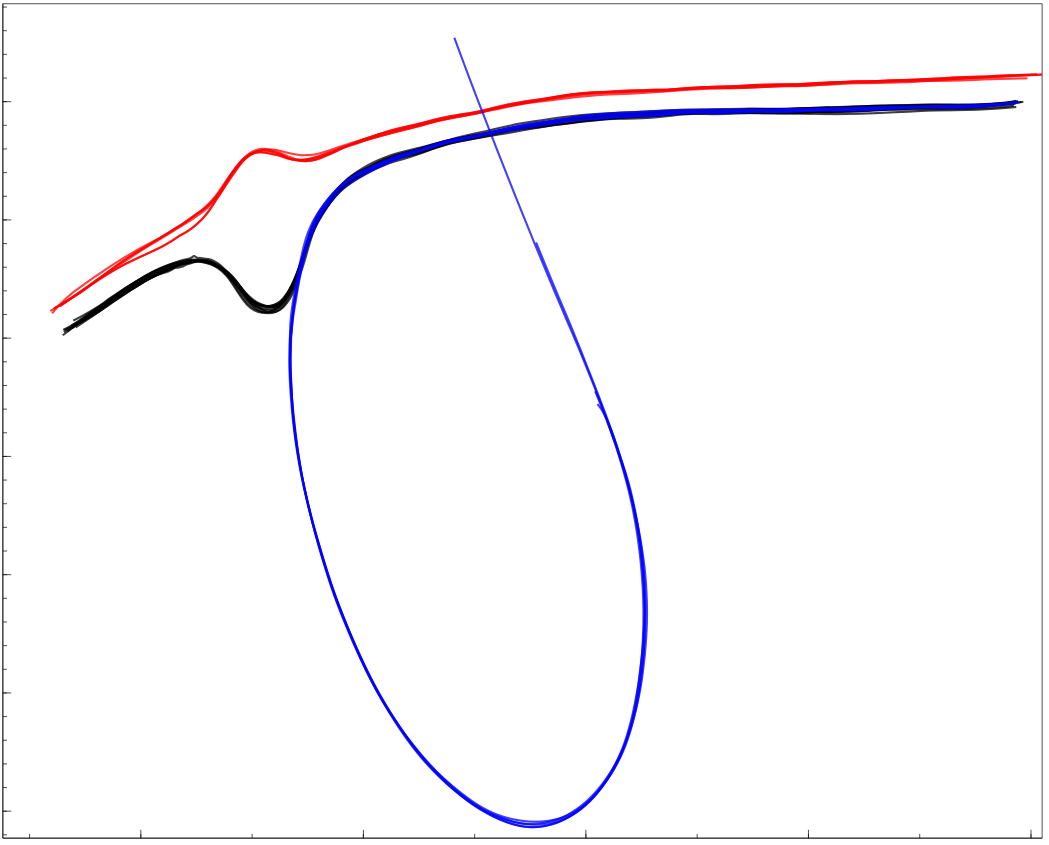
\includegraphics[align=c, width=0.35\linewidth]{resources/img/results/Steinheim/filteredClusters_03}
    }}
    \qquad \qquad
    \subfloat[]{{
        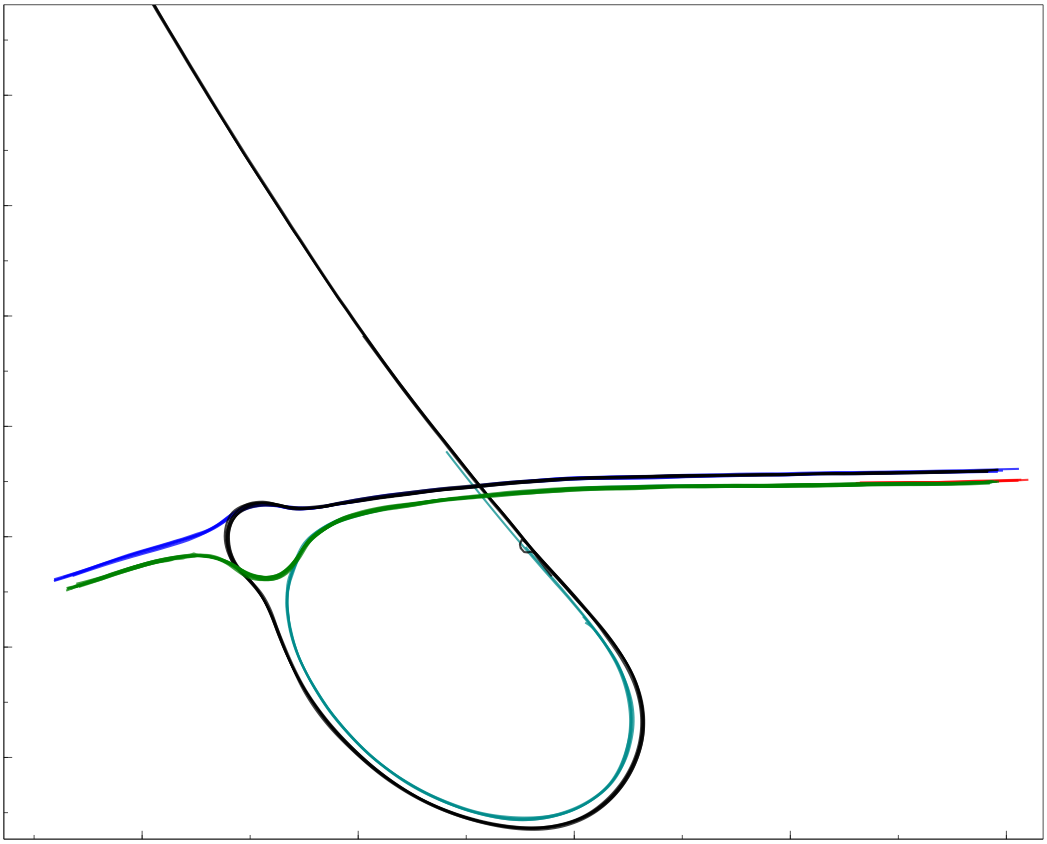
\includegraphics[align=c, width=0.35\linewidth]{resources/img/results/Steinheim/filteredClusters_015}
    }}
    \caption[Ergebnisse Clusteranalyse Steinheim]
            {a) Ergebnis Standard-Clusteranalyse ($\epsilon_{DBSCAN} = 0.3$),
            b) Ergebnis Clusteranalyse nach manuelle Anpassung von $\epsilon_{DBSCAN}$ auf 0.1}
    \label{fig:results_clusters_steinheim}
\end{figure}

Da die Spur-Geometrien, welche anhand der in Abbildung \ref{fig:results_clusters_steinheim} a) zu sehenden
Cluster gebildet werden, jeweils nur eine Fahrspur des Straßenabschnittes \textit{Steinheim} beschreiben,
existieren in den abgeleiteten Weg-Zeit-Trajektorien keine Überschneidungen. Die Spurerkennung wird daher
nicht automatisch unter Verwendung eines angepassten Parameters wiederholt (siehe Abschnitt \ref{sec:real1_adjustment_clustering_parameter}).
Um die zweite, nach hinten verlaufende Fahrspur zu identifizieren, muss $\epsilon_{DBSCAN}$ manuell angepasst werden.
Das Ergebnis ist in Abbildung \ref{fig:results_clusters_steinheim} b) dargestellt.
Da die Trajektorien auf den nach hinten verlaufenden Fahrspuren aufgrund der drei Brücken
(siehe Abbildung \ref{fig:results_horizon_problem}) sehr viele Unterbrechungen
aufweisen, kann der Clusteralgorithmus für die linke Spur zudem nur ein Cluster identifizieren, welches bis
knapp vor die Brücken verläuft.

Für die Clusteranalyse kann zusammenfassend festgehalten werden, dass sie gut funktioniert, wenn ausreichend
intakte Trajektorien zur Beschreibung einer Spur vorliegen. Dank sorgfältig gewählter Standardparameter
und einer automatischen Parametrisierung können in den meisten Fällen die korrekten Spur-Cluster voll automatisch
ermittelt werden. Nur in Ausnahmefällen muss die Clusteranalyse manuell konfiguriert werden.

\section{Evaluierung der Spur-Geometrie-Bestimmung}

Nach der Clusteranalyse werden anhand der identifizierten Spur-Cluster die Geometrien der Fahrspuren
bestimmt. Die hierzu angewandten Verfahren sind in Abschnitt \ref{cha:lane_definition} beschrieben.

Wurden im vorherigen Schritt Trajektorie-Cluster für die in einer Aufnahme enthaltenen Fahrspuren identifiziert,
so können auf Basis dieser meist zuverlässige Spur-Geometrien abgeleitet werden.
In Abbildung \ref{fig:results_laneGeometries} sind beispielhaft Spur-Geometrien aus drei unterschiedlichen Datensätzen dargestellt.

\begin{figure}
    \centering
    \subfloat[Heilbronner-Straße]{{
        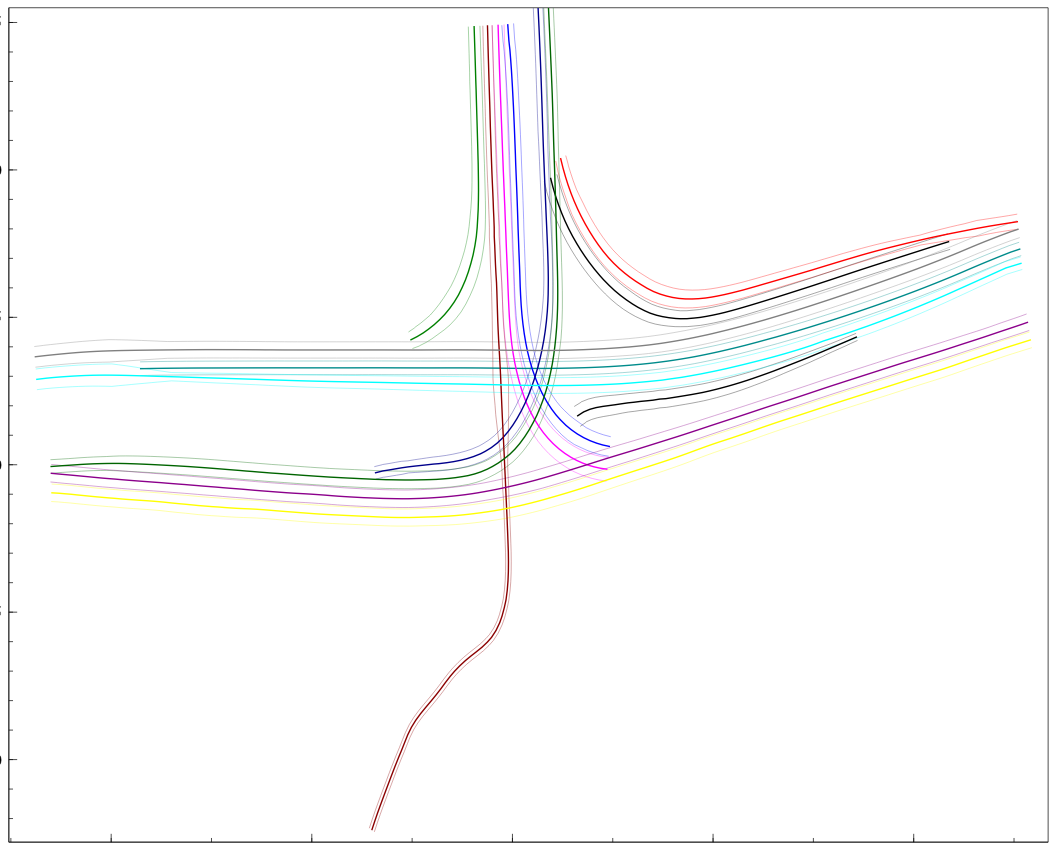
\includegraphics[align=c, width=0.45\linewidth]{resources/img/results/Heilbronner/improvedLanes_Heilbronner}
    }}
    \qquad
    \subfloat[Düsseldorf]{{
        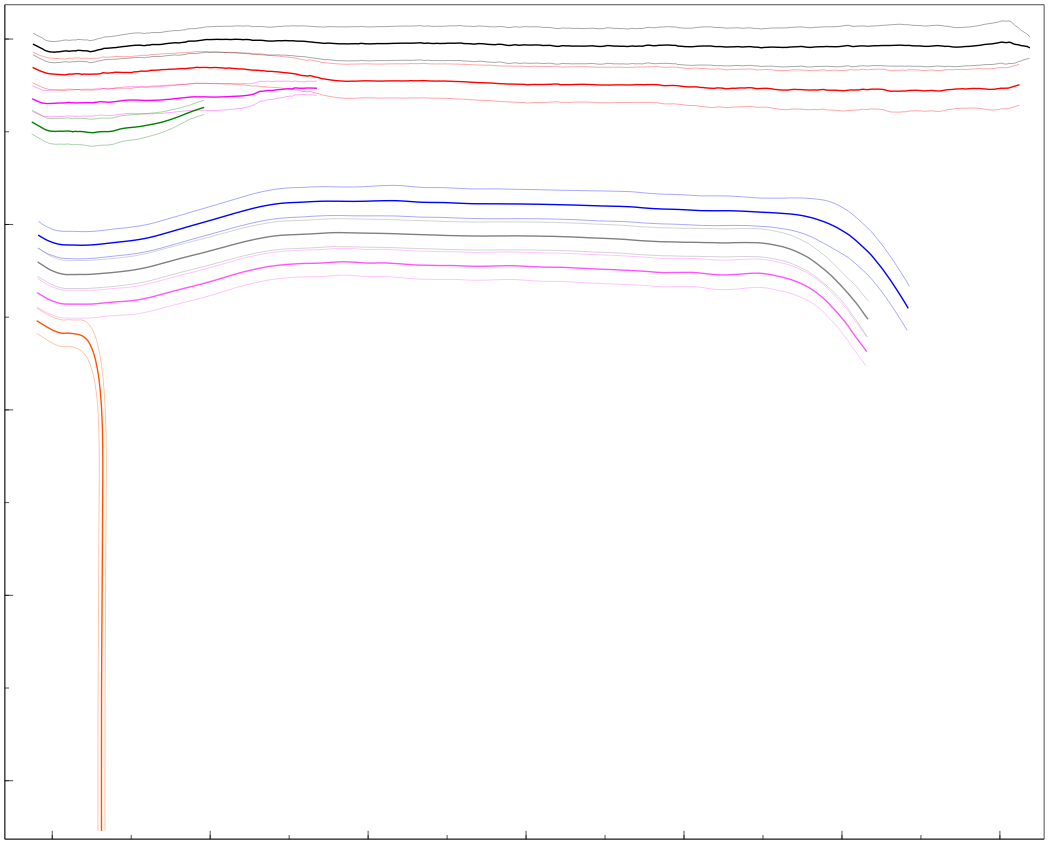
\includegraphics[align=c, width=0.45\linewidth]{resources/img/results/Duesseldorf/improvedLanes_Duesseldorf}
    }}
    \hfill
    \subfloat[Steinheim]{{
        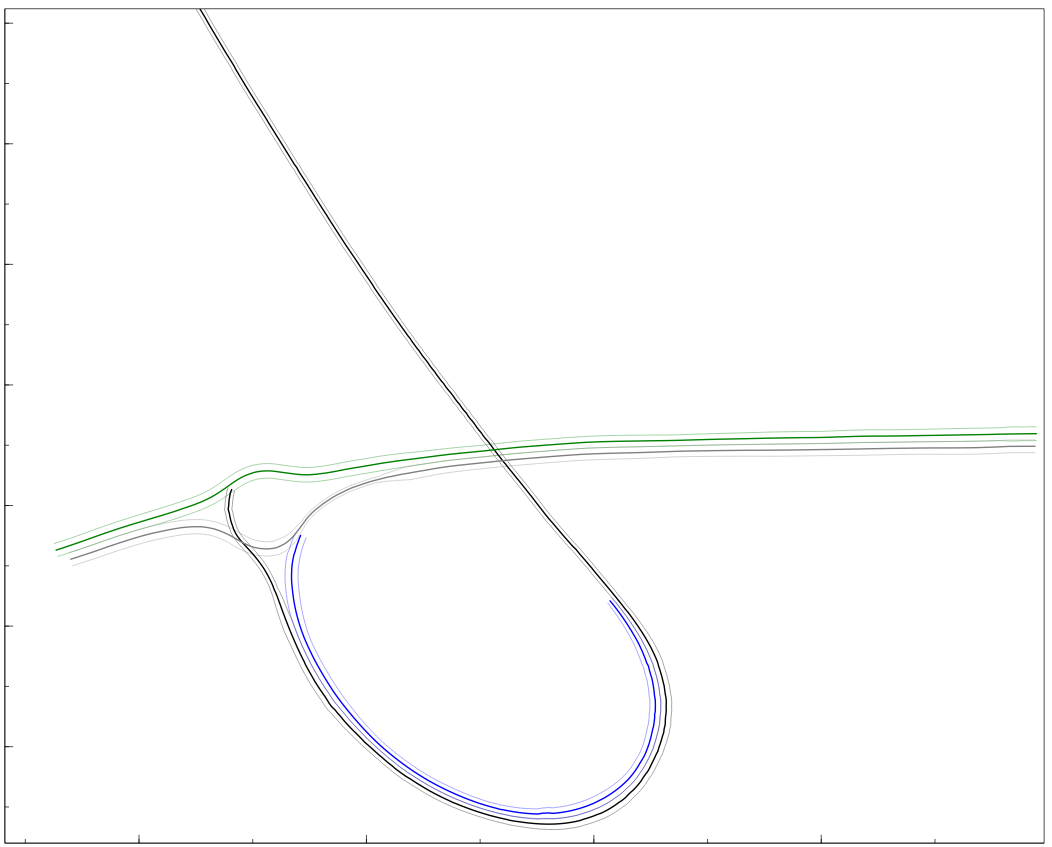
\includegraphics[align=c, width=0.45\linewidth]{resources/img/results/Steinheim/improvedLanes2}
    }}
    \caption[Ergebnisse der Spur-Geometrie-Bestimmung]
            {Ergebnisse der Spur-Geometrie-Bestimmung von verschiedenen Straßenabschnitten}
    \label{fig:results_laneGeometries}
\end{figure}

Anhand der abgebildeten Spur-Geometrien ist zu erkennen, dass das in Abschnitt \ref{cha:lane_definition}
beschriebene Verfahren gute Ergebnisse in unterschiedlichen Situationen liefert.
Plot a) zeigt die Spur-Geometrien, welche im Fall des Datensatzes der Heilbronner-Straße bestimmt werden.
Für jedes Spurcluster, welches in Abbildung \ref{fig:results_clusters_heilbronner} a) zu sehen ist, wurde eine Geometrie erstellt.
Es ist zudem zu sehen, dass die Fahrspuren partitioniert wurden, um Überlagerungen zu vermeiden.
Plot b) zeigt, dass Spur-Geometrien auch korrekt bestimmt werden, wenn in einer Aufnahme
Fahrbahnerweiterung existieren, wie dies im \textit{Düsseldorf}-Datensatz der Fall ist.
Anhand von Plot c), welcher die für den Datensatz \textit{Steinheim} ermittelten Spur-Geometrien zeigt, wird
außerdem deutlich, dass auch die Geometrien kreisförmiger Fahrspuren und Kreisverkehre bestimmt werden können.

Ein Problem, welches bei der Bestimmung der Spur-Geometrien auftreten kann, ist in Abbildung
\ref{fig:results_defekts_laneGeos} dargestellt.

\begin{figure}[H]
    \centering
    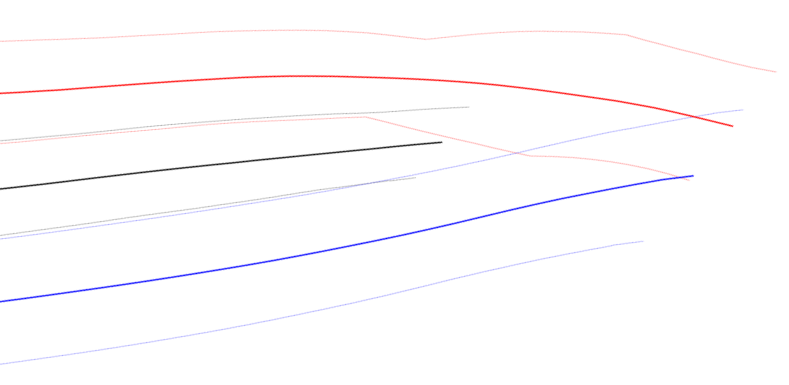
\includegraphics[width=0.5\linewidth]{resources/img/results/Defekte/Defekt_Part2}
    \caption{Partitionierungsproblem in den Spur-Geometrien}
    \label{fig:results_defekts_laneGeos}
\end{figure}

Das Beispiel zeigt einen Ausschnitt aus den Spur-Geometrien des Datensatzes \textit{Heilbronner-Straße}.
Auf dem entsprechenden Straßenabschnitt (vergleiche Abb. \ref{fig:results_lanes2} b)),
auf welchem sich die Spuren befinden, verbreitert sich am rechten Rand der Aufnahme die Fahrbahn nach oben hin.
Es entstehen zwei neue Fahrspuren. In den partitionierten Spur-Geometrien sollte daher eigentlich die
oberer Spur (rot) aus der mittlere Spur (schwarz) hervorgehen, welche wiederum selbst aus der unteren
Spur (blau) hervorgeht.
Wie in der Abbildung zu sehen ist, wird allerdings die mittlere Spur partitioniert
und die obere bleibt erhalten. Hier trifft der in Abschnitt \ref{sec:real2_lane_partitioning} beschrieben
Algorithmus eine falsche Partitionierungsentscheidung.

Partitionierungsprobleme können in ähnlicher Art gelegentlich auftreten. Der Grund hierfür
ist, dass es sehr schwierig ist, ein Verfahren zu definieren, welches in allen möglichen
Spurüberlagerungs-Konstellationen die richtige Entscheidung trifft.
Ein menschlicher Betrachter kann bei der Überlagerung zweier Spuren zwar meist intuitiv feststellen, welche
partitioniert werden muss, einem Algorithmus dies beizubringen, ist allerdings schwierig,
da die Entscheidung von vielen verschiedenen, situationsbezogenen Kriterien abhängt.

Der verwendete Partitionierungsansatz liefert, wie angestrebt, in der Mehrzahl der Fälle eine gute Lösung.
Es musste bei der Entwicklung darauf geachtet werden, das keine Verfahren erstellt wird, welches zu sehr
auf wenige Szenarien angepasst ist. 
Häufig gibt es bei der Teilung der Spuren auch kein eindeutiges ``Richtig'' oder ``Falsch''.
Welche Spur erhalten bleiben soll, ist dann Interpretationssache. Daher, und da die Fehler
leicht über die Oberfläche der \textit{Vehicle-Tracker} Anwendung korrigiert werden können, wurde der verwendete
Algorithmus hier nicht weiter angepasst.

\section{Ergebnisse der Spurerkennung}

Nachdem in den vorherigen Abschnitten auf die Fähigkeiten und Probleme der drei Hauptschritte des
Spurerkennungsverfahrens eingegangen wurde, werden nun Ergebnisse in Form von Screenshots vorgestellt.
In ihnen sind die automatisch erkannten und erstellten Spuren zu sehen, wie sie in der Anwendung
\textit{Vehicle-Tracker} dargestellt sind.

Die ersten zwei Screenshots, welche in Abbildung \ref{fig:results_lanes1} dargestellt sind, zeigen die ermittelten
Spuren für die Datensätze \textit{Esslingen} und \textit{Düsseldorf}.
In den Aufnahmen ist zu erkennen, dass die erstellten Fahrspuren gut mit den realen Verläufen der
Spuren auf der Fahrbahn übereinstimmen.
Dies gilt auch im Fall des Datensatzes \textit{Düsseldorf}, obwohl die hier detektierten Fahrzeugpositionen
aufgrund des niedrigen Aufnahmewinkels nicht immer in der Nähe der Spurmitte liegen
(siehe Abschnitt \ref{sec:grund_challenges_reconstruction}).

\begin{figure}[H]
    \centering
    \subfloat[Fahrspuren Esslingen]{{
        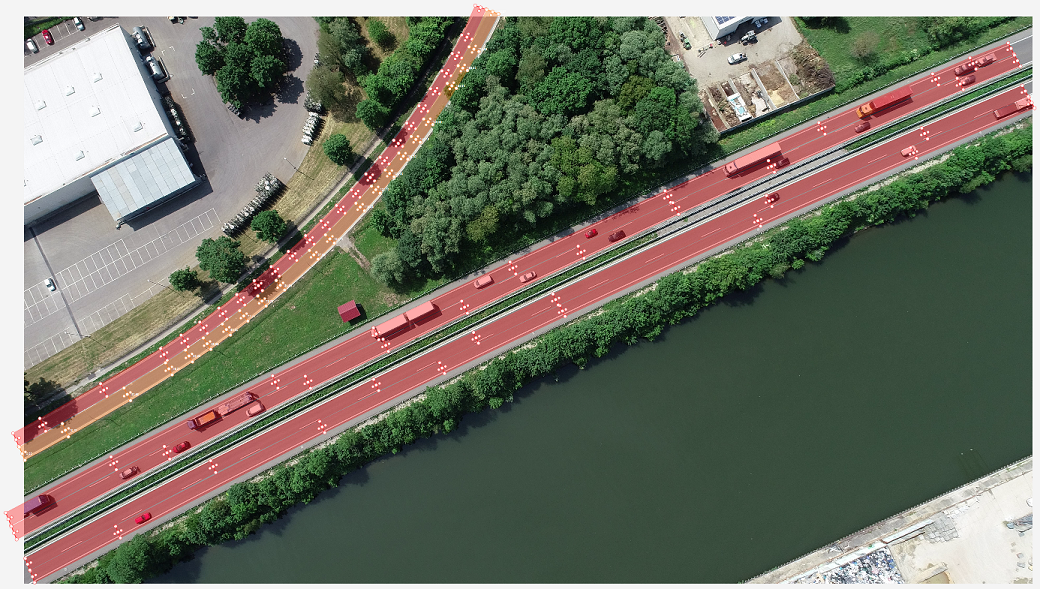
\includegraphics[align=c, width=0.5\linewidth]{resources/img/results/Lanes/Entennest_Lanes}
    }}
    \subfloat[Fahrspuren Düsseldorf]{{
        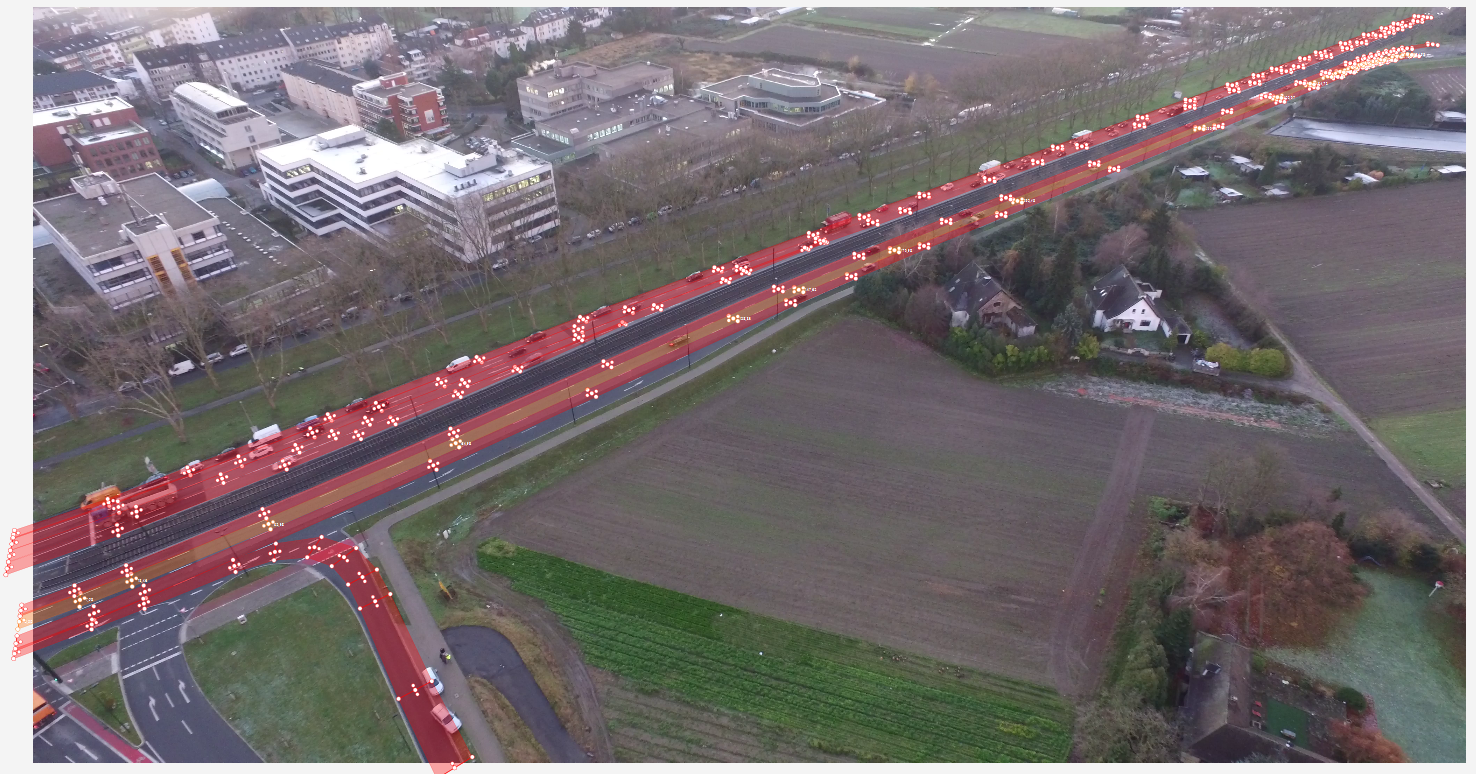
\includegraphics[align=c, width=0.5\linewidth]{resources/img/results/Lanes/Duesseldorf_Lanes}
    }}
    \caption{Erkannte Fahrspuren auf geraden Straßenabschnitten}
    \label{fig:results_lanes1}
\end{figure}

In Abbildung \ref{fig:results_lanes2} sind die erkannten Spuren der Datensätze \textit{Neckartor} und \textit{Heilbronner-Straße}
dargestellt. Auch hier stimmen die Spur-Geometrien gut mit den realen Spur-Ausmaßen überein. Zudem wird deutlich,
dass sowohl die Partitionierung der Spuren als auch das Angleichen benachbarter Spurenden die gewünschten Resultate liefern.
Im Fall der Heilbronner-Straße ist nun auch zu sehen, dass im unteren rechten Bereich keine Spur erkannt wird.
Der Grund hierfür wurde in Abschnitt \ref{sec:results_eval_clustering} beschrieben.

\begin{figure}[H]
    \centering
    \subfloat[Fahrspuren Neckartor]{{
        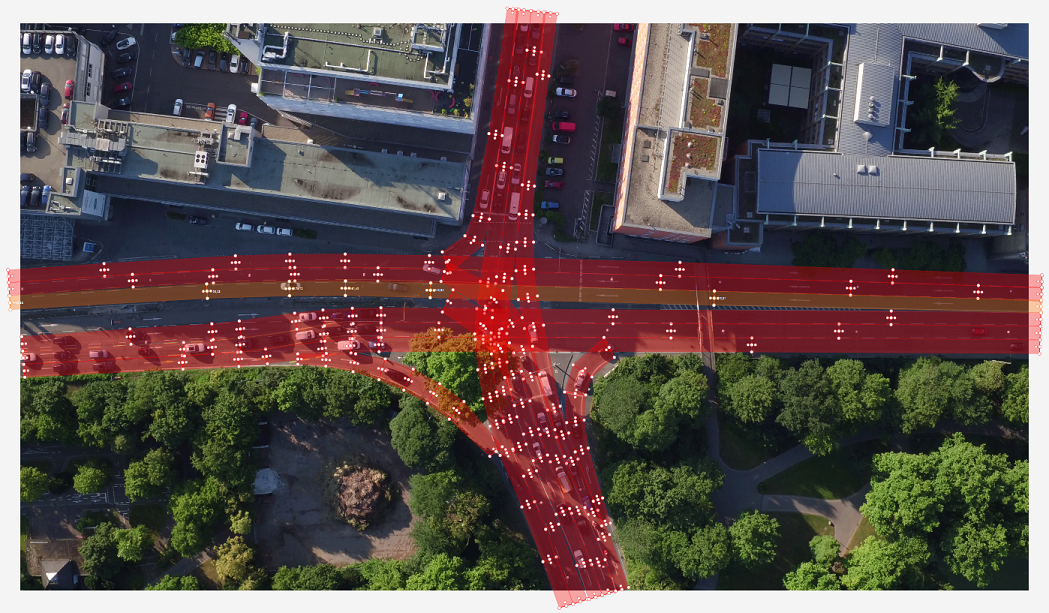
\includegraphics[align=c, width=0.5\linewidth]{resources/img/results/Lanes/Neckartor_Lanes}
    }}
    \subfloat[Fahrspuren Heilbronner-Straße]{{
        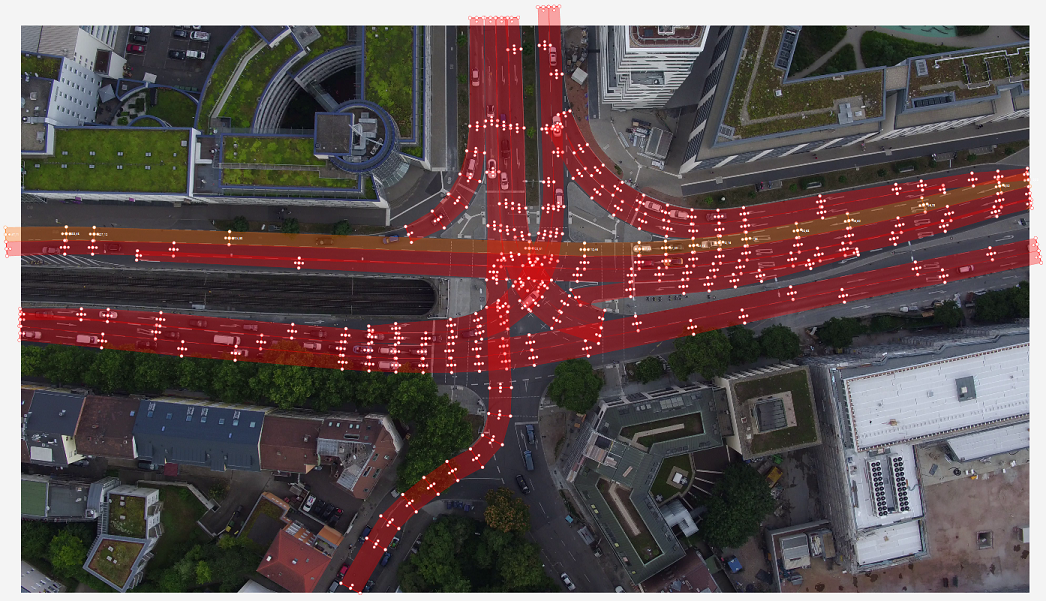
\includegraphics[align=c, width=0.5\linewidth]{resources/img/results/Lanes/Heilbronner_Lanes}
    }}
    \caption{Erkannte Fahrspuren auf Kreuzungen}
    \label{fig:results_lanes2}
\end{figure}

Der Screenshot in Abbildung \ref{fig:results_lanes3} zeigt die erkannten Fahrspuren im Datensatz \textit{Steinheim}.
Dieses Beispiel zeigt, dass Fahrspuren auch in Straßenabschnitten mit Kreisverkehren oder kreisförmigen Spuren
erkannt werden. Auch hier stimmen, trotz des niedrigen Aufnahmewinkels, die Fahrspuren weitestgehend
mit den realen Fahrbahnverläufen überein. Der frühe Abbruch der linken, nach oben verlaufenden Fahrspur
lässt sich auf die Unterbrechungen der Trajektorien in diesem Bereich zurückführen.

\begin{figure}[H]
    \centering
    \subfloat[Fahrspuren Steinheim]{{
        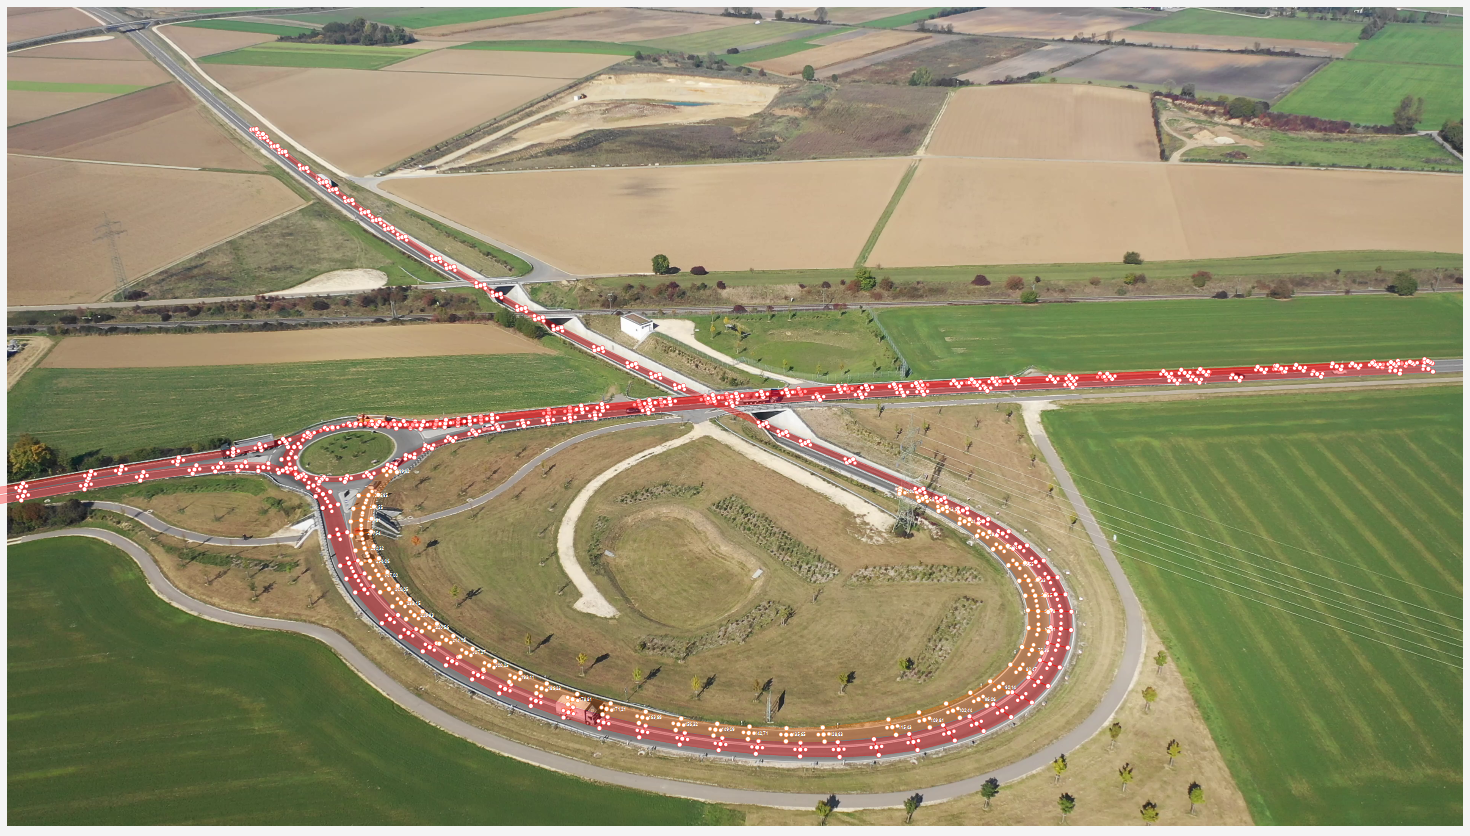
\includegraphics[align=c, width=0.6\linewidth]{resources/img/results/Lanes/Steinheim_Lanes}
    }}
    \caption{Erkannte Fahrspuren auf kreisförmigen Fahrbahnen}
    \label{fig:results_lanes3}
\end{figure}

Die oben abgebildeten und beschriebenen Ergebnisse zeigen, dass der entwickelte Spurerkennungsalgorithmus die in
Abschnitt \ref{sec:requirements} aufgestellten Anforderungen erfüllt.
Es können Fahrspuren in Straßen mit unterschiedlichen Topologien erkannt werden. Diese stimmen
mit den realen Spur-Geometrien meist gut überein. Auch bei niedrigen Aufnahmewinkeln können
Fahrspuren aus den Trajektorien abgeleitet werden, welche den Verlauf der Fahrbahnen ausreichend genau
beschreiben. Mit den meisten Defekten und Ausreißern in den Trajektorien kann umgegangen werden.
Schwierigkeiten hat das Verfahren, wenn die Mehrzahl der Trajektorien einer Fahrspur
Unterbrechungen aufweisen.
%!TEX root = ../Thesis.tex

\chapter{Zusammenfassung und Ausblick}
\label{cha:end}

Am Ende dieser Arbeit wird nun der Inhalt der vorliegenden Arbeit und deren Ergebnisse noch
zusammengefasst. Zudem wird ein Ausblick gegeben, welche Optimierungen beziehungsweise
Weiterentwicklungen in Zukunft an der Spurerkennung noch vorgenommen werden können.

\section{Zusammenfassung}

Im Rahmen dieser Arbeit wurde ein Verfahren zur automatischen Erkennung von Fahrspuren in Videoaufnahmen
anhand von Trajektoriedaten entwickelt.

Eine initiale Untersuchung der Literatur im Bereich Fahrspurerkennung und Trajektorieauswertung
machte deutlich, dass ein Algorithmus mit den gewünschten Eigenschaften weitestgehend neu entwickelt werden muss.
Die in den verwandten Arbeiten vorgestellten Verfahren eignen sich meist nur zur Erkennung von Fahrspuren
in bestimmten Straßentopologien. Außerdem stimmen die von ihnen ermittelten Spur-Geometrien nur selten
mit den realen Abmaßen der Fahrspuren auf der Straße überein.
Der im Rahmen dieser Thesis entwickelte Spurerkennungsalgorithmus sollte beide diese Anforderungen erfüllen.

Das erstellte Verfahren besteht aus mehreren, aufeinander aufbauenden Verarbeitungsschritten. Die aus den
Luftaufnahmen extrahierten Fahrzeugtrajektorien werden in einer ersten Vorverarbeitung weitestgehend von
Ausreißern und Defekten befreit. Die nach diesem Schritt vorliegenden Trajektorien beschreiben
ununterbrochene Bewegungsbahnen von Fahrzeugen durch einen bestimmten Straßenabschnitt.
Mittels einer Clusteranalyse werden anschließend Gruppen von Trajektorien identifiziert, welche Bewegungen
auf der selben Fahrspur beschreiben.
Diese Spurcluster dienen als Basis für die Bestimmung der Spur-Geometrien. Für jedes Cluster wird eine
Spurmittellinie und Hüll-Linien definiert, welche den Verlauf und die Breite der Fahrspur beschreiben.
Die Spur-Geometrien werden zudem noch partitioniert, um Überlagerungen von Spuren zu entfernen.
Eine finale Optimierung der Spur-Geometrien sorgt dafür, dass die algorithmisch ermittelten Fahrspuren
mit den realen Spurabmaßen bestmöglich übereinstimmen. 

In Kapitel \ref{cha:results} wurden die Fähigkeiten und noch existierenden Schwächen des entwickelten
Verfahrens evaluiert. Zudem wurden Ergebnisse der Spurerkennung von unterschiedlichen Straßenabschnitten
vorgestellt. Es wurde deutlich, dass das Verfahren Fahrspuren in den meisten Situationen zuverlässig
ermitteln kann. Die erstellten Spur-Geometrien stimmen mit den realen Fahrbahnverläufen gut überein.
Kleine Abweichungen sind in der Regel zu vernachlässigen, da sie die Zuweisung von Fahrzeugen zu Fahrspuren
nicht beeinträchtigen.
Deutlich wurde allerdings auch, dass die größte Schwäche des entwickelten Spurerkennungsalgorithmus
dessen Abhängigkeit von einer ausreichenden Anzahl ununterbrochener Trajektorien ist. Wenn für eine
Fahrspur eines Straßenabschnitts nicht ausreichend Trajektorien vorliegen, oder die existierenden an sehr
unterschiedlichen Positionen unterbrochen sind, gelingt es dem Algorithmus nicht für die Spuren
Spur-Geometrien zu bestimmen.

Der entwickelte Algorithmus wurde in die Anwendung \textit{Vehicle-Tracker} integriert,
welche im MEC-View Teilprojekt ``Luftbeobachtung'' zur Analyse des Fahrverhaltens von Verkehrsteilnehmern
eingesetzt wird. Dank der automatischen Spurerkennung können in Zukunft Luftaufnahmen des Straßenverkehrs
schneller ausgewertet werden.

\section{Ausblick}

Der im Rahmen dieser Thesis entwickelte Spurerkennungsalgorithmus ermöglicht die schnellere Auswertung
des Fahrverhaltens von Fahrzeugen in Luftaufnahmen. Mithilfe der ermittelten Spurinformationen können
unter anderem Überhol- und Spurwechselvorgänge sowie das Verhalten der Fahrzeuge auf einer Spur
untereinander untersucht werden.

Die Spur-Geometrien könnten in Zukunft zudem zur Evaluierung der Qualität der Fahrzeugerkennung und Verfolgung
und insbesondere zur Identifikation von Ausreißern eingesetzt werden. Da die relevanten Fahrzeuge sich
auf den Fahrbahnen eines Straßenabschnittes befinden, kann anhand der Spurinformationen ermittelt werden, 
welche Trajektorien außerhalb dieser liegen und daher vermutlich Ausreißer sind.

Die Zuverlässigkeit der Fahrspurerkennung könnte in Zukunft durch die Identifizierung und Implementierung
eines alternativen Verfahrens zur Clusteranalyse weiter gesteigert werden.
Der derzeit
eingesetzte Ansatz, welcher komplette Trajektorien gruppiert, liefert zwar in der Mehrzahl der Fälle
gute Ergebnisse, ist jedoch auch dafür verantwortlich, dass in manchen Situationen Fahrspuren nicht erkannt werden.
Ein alternatives Verfahren könnte sich beispielsweise an der Arbeit von \cite[]{Xu2015} orientieren, in welcher
anhand der Trajektoriedaten eine \textit{``Heat-Map''} erstellt wird, aus welcher anschließend ``Mittellinien''
anhand eines \textit{``Adaptive Multi-Kernel-Based Shrinkage''}-Algorithmus extrahiert werden.
Hierbei fallen Unterbrechungen von Trajektorien nicht ins Gewicht.
Da die einzelnen Schritte der Spurerkennung unabhängig voneinander arbeiten, könnte ein
solches alternatives Clusterverfahren mit geringen Auswirkungen auf den Rest des Algorithmus integriert werden.

% % %%%%%% Literaturverzeichnis (darf im deutschen nicht in den Anhang!)
% Einfaches Literaturverzeichnis
% \input{chapters/bibEinfach}
% Literaturverzeichnis mit Bibtex
\bibliography{bib/sources}

\printglossary

% % %%%%%% Anhang
\appendix
% %!TEX root = ../Thesis.tex

\chapter{Anhang - Verwendete Datensätze}
\label{cha:anhang_a}

Nachfolgend sind Aufnahmen der in dieser Arbeit verwendeten Luftaufnahmen zu sehen.

\subsection*{Datensatz Entennest}

\begin{figure}[H]
\centering
    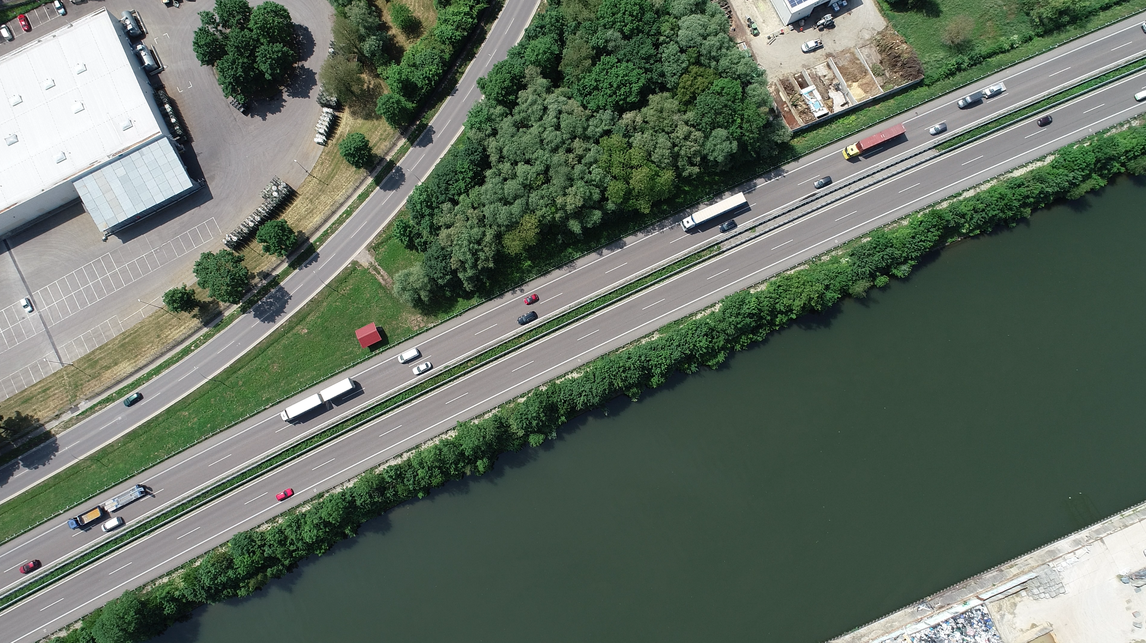
\includegraphics[width=0.6\linewidth]{resources/img/Anhang/Entennest}
\caption{Staßenabschnitt Aufnahme Entennest}
\label{fig:anhang_ds_entennest}
\end{figure}

\subsection*{Datensatz Neckartor}

\begin{figure}[H]
\centering
    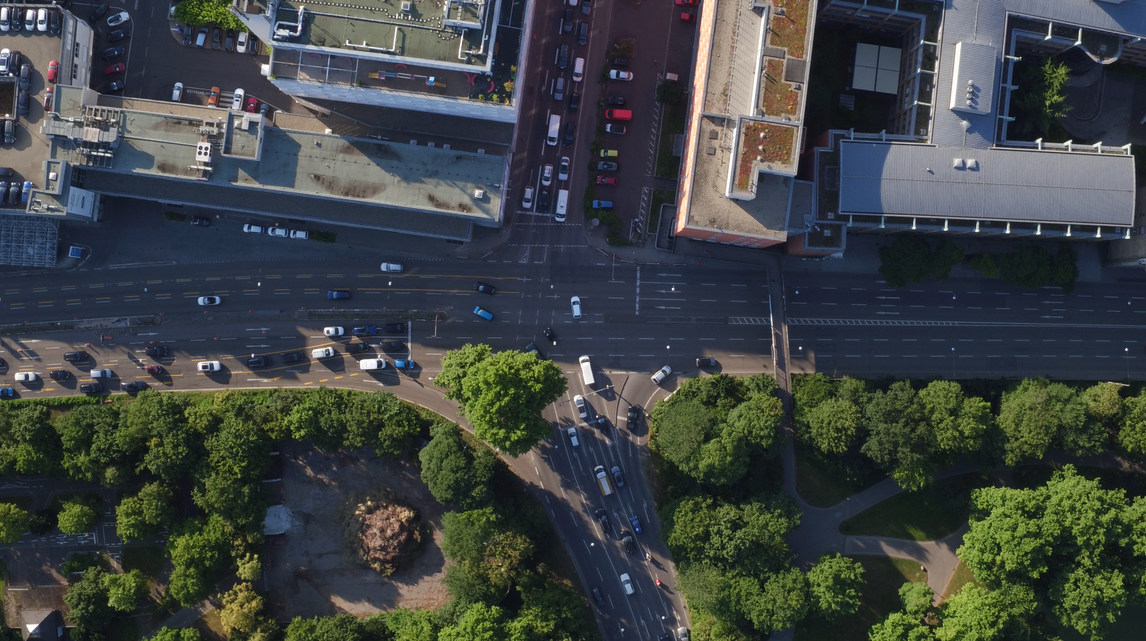
\includegraphics[width=0.6\linewidth]{resources/img/Anhang/Neckartor}
\caption{Staßenabschnitt Aufnahme Neckartor}
\label{fig:anhang_ds_neckartor}
\end{figure}

\subsection*{Datensatz Heilbronner-Straße}

\begin{figure}[H]
\centering
    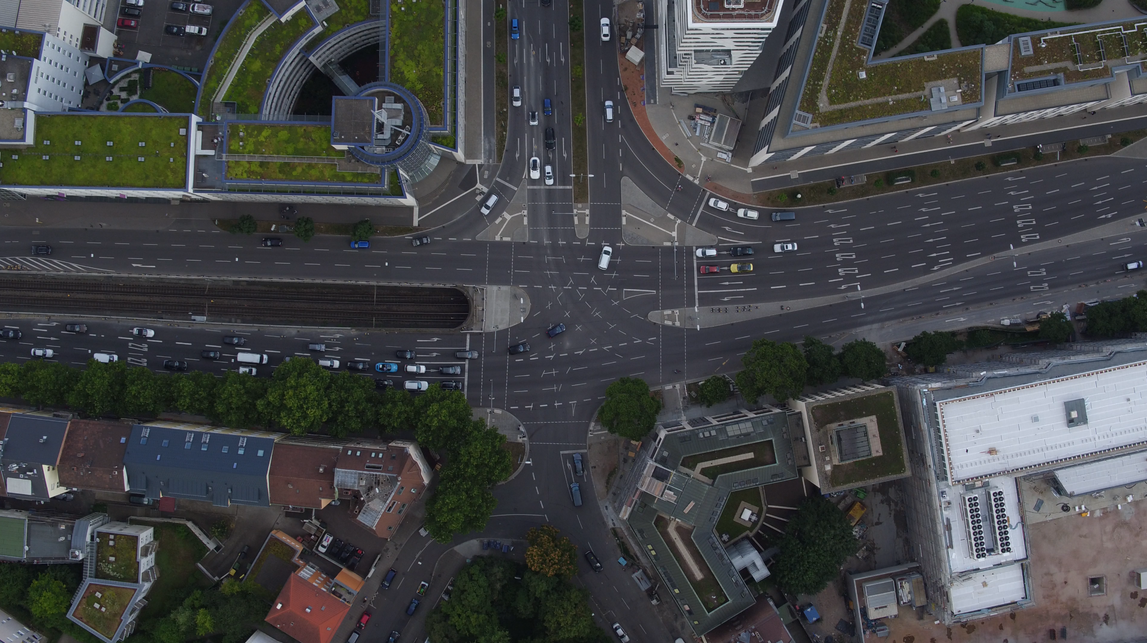
\includegraphics[width=0.6\linewidth]{resources/img/Anhang/Heilbronner}
\caption{Staßenabschnitt Aufnahme Heilbronner-Straße}
\label{fig:anhang_ds_heilbronner}
\end{figure}

\subsection*{Datensatz Düsseldorf}

\begin{figure}[H]
\centering
    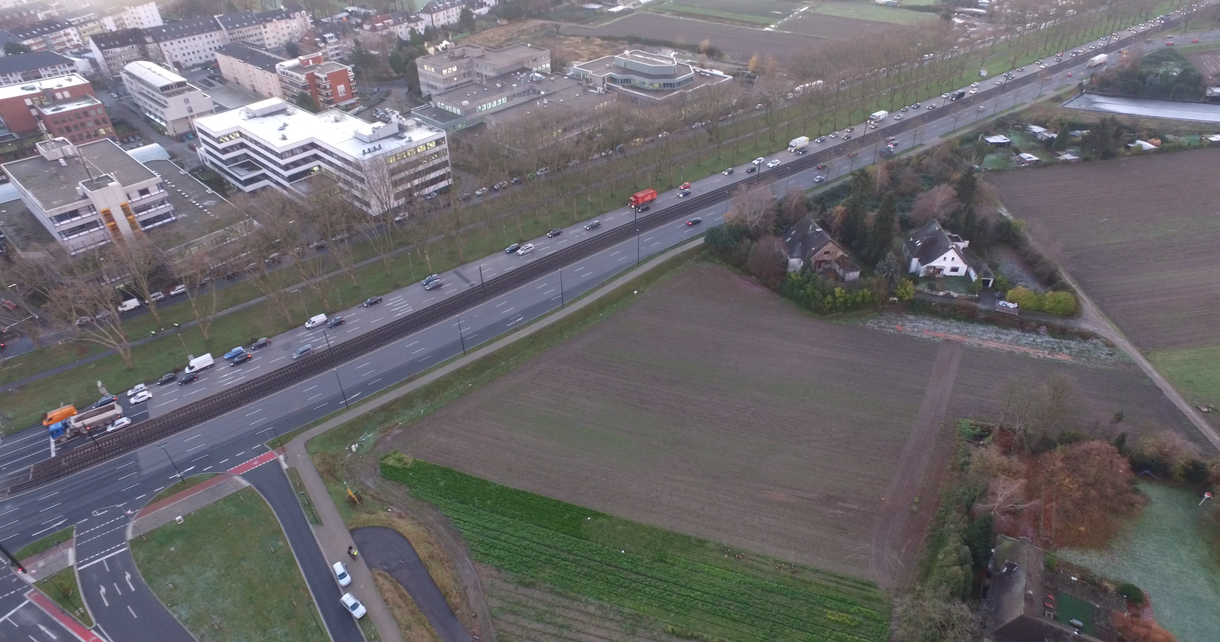
\includegraphics[width=0.6\linewidth]{resources/img/Anhang/Duesseldorf}
\caption{Staßenabschnitt Aufnahme Düsseldorf}
\label{fig:anhang_ds_duesseldorf}
\end{figure}

\subsection*{Datensatz Steinheim}

\begin{figure}[H]
\centering
    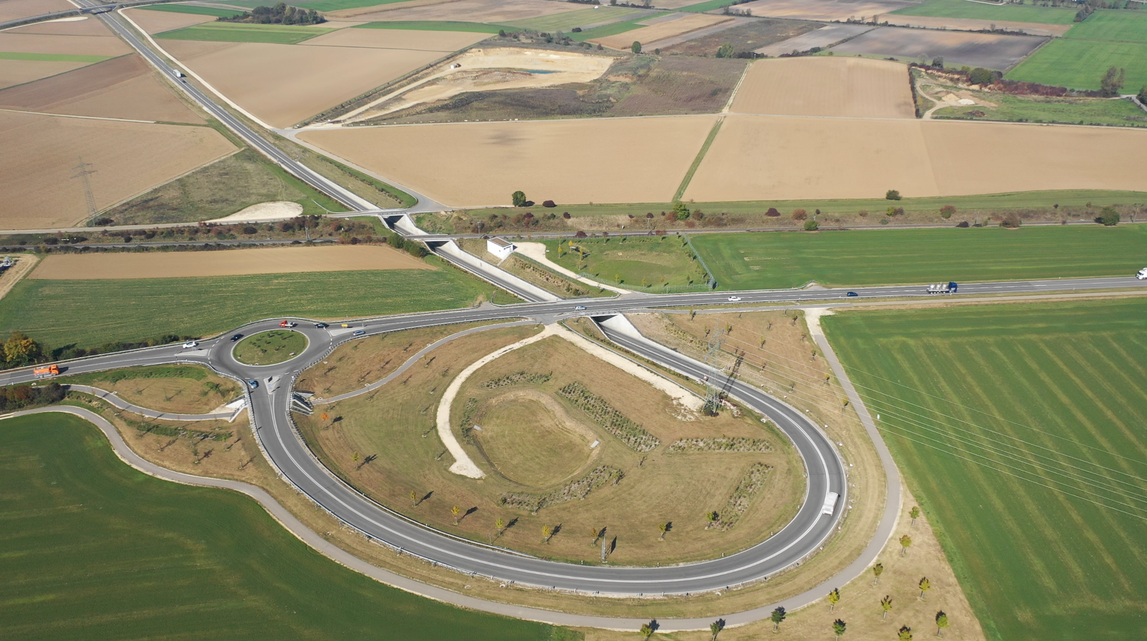
\includegraphics[width=0.6\linewidth]{resources/img/Anhang/Steinheim}
\caption{Staßenabschnitt Aufnahme Steinheim}
\label{fig:anhang_ds_steinheim}
\end{figure}

% %  Inhalt ENDE %%%%%%%%%%%%%%%%%%%%%%%%%%%%%%%%%%%%%%%%%%%%%%%%%%%%%%%%%%
\end{document}
